% =====================================================================
%  BioBot-Rescue -- Esquema de investigacion del proyecto final
%  O26-LRT3032-2 Sistemas Embebidos -- UDLAP
%  Roberto Orozco Ramirez (184595), Adam Del Pozo Ontiveros (185611) y
%  Enrique Bernal Martin Prieto (184878)
%
%  Compilar con ..\compilar.ps1 (dos pasadas de pdflatex; latexmk no sirve:
%  este MiKTeX no trae Perl). Las figuras de figs\ las genera
%  ..\modelo\figuras.py a partir de la simulacion y de los datos citados.
% =====================================================================
\documentclass[11pt,letterpaper]{article}

\usepackage[spanish,es-tabla,es-noshorthands]{babel}
\usepackage[T1]{fontenc}
\usepackage[utf8]{inputenc}
\usepackage{lmodern}
\usepackage[margin=2.1cm,top=2.4cm,bottom=2.3cm]{geometry}
\usepackage{setspace}
\usepackage{microtype}
\usepackage{amsmath}
\usepackage{amssymb}
\usepackage{siunitx}
\usepackage{graphicx}
\usepackage{array}
\usepackage{tabularx}
\usepackage{booktabs}
\usepackage{multirow}
\usepackage{enumitem}
\usepackage[table]{xcolor}
\usepackage[most]{tcolorbox}
\usepackage{titlesec}
\usepackage{fancyhdr}
\usepackage{ragged2e}
\usepackage{tikz}
\usetikzlibrary{positioning,arrows.meta,calc,fit,shapes.geometric,automata}
\usepackage{caption}
\usepackage{subcaption}
\usepackage{float}
\usepackage{needspace}
\usepackage{xurl}
\usepackage{lastpage}
\usepackage[colorlinks=true,linkcolor=blue!50!black,urlcolor=blue!50!black,citecolor=blue!50!black]{hyperref}
\usepackage{bookmark}

\sisetup{output-decimal-marker={.},group-separator={\,},range-phrase={--},range-units=single}
\setstretch{1.08}
\setlength{\parindent}{0pt}
\setlength{\parskip}{4pt}
\setlength{\headheight}{26pt}
\setlength{\emergencystretch}{3em}
\raggedbottom
\renewcommand{\arraystretch}{1.15}
\captionsetup{font=small,labelfont={bf,color=Primary},skip=4pt}

% ---- paleta (la de los reportes de práctica) ----
\definecolor{Primary}{HTML}{0E2A47}
\definecolor{Secondary}{HTML}{1D6FA5}
\definecolor{Accent}{HTML}{D98B12}
\definecolor{AccentSoft}{HTML}{FFF2DD}
\definecolor{SoftBlue}{HTML}{ECF3FA}
\definecolor{SoftGray}{HTML}{F5F7FA}
\definecolor{SoftMint}{HTML}{EAF8F1}
\definecolor{Good}{HTML}{1D7A46}
\definecolor{Bad}{HTML}{B03A2E}
\definecolor{TableHead}{HTML}{D7E7F7}
\definecolor{TextDark}{HTML}{1E293B}

\titleformat{\section}
  {\Large\bfseries\color{Primary}}
  {\colorbox{Primary}{\color{white}\strut\hspace{0.5em}\thesection\hspace{0.5em}}}{0.7em}{}
  [\vspace{0.1em}\color{Secondary}\titlerule]
\titleformat{\subsection}
  {\large\bfseries\color{Secondary}}
  {\colorbox{Secondary!15}{\color{Primary}\strut\hspace{0.4em}\thesubsection\hspace{0.4em}}}{0.6em}{}
\titleformat{\subsubsection}{\normalsize\bfseries\color{Primary}}{}{0pt}{}
\titlespacing*{\section}{0pt}{1.0em}{0.6em}
\titlespacing*{\subsection}{0pt}{0.8em}{0.4em}
\titlespacing*{\subsubsection}{0pt}{0.6em}{0.2em}

\newtcolorbox{infobox}[1][]{colback=SoftBlue,colframe=Secondary,boxrule=0.9pt,
  arc=2.2mm,left=2mm,right=2mm,top=1.5mm,bottom=1.5mm,breakable,#1}
\newtcolorbox{alertbox}[1][]{colback=AccentSoft,colframe=Accent,boxrule=0.9pt,
  arc=2.2mm,left=2mm,right=2mm,top=1.5mm,bottom=1.5mm,breakable,#1}
\newtcolorbox{goodbox}[1][]{colback=SoftMint,colframe=Good,boxrule=0.9pt,
  arc=2.2mm,left=2mm,right=2mm,top=1.5mm,bottom=1.5mm,breakable,#1}

\newcommand{\sig}[1]{\texttt{#1}}
\newcommand{\especie}{\textit{Gromphadorhina portentosa}}
\newcommand{\Gp}{\textit{G.~portentosa}}
% Etiqueta de origen de un parámetro: F fuente publicada, D derivado, S supuesto
\newcommand{\orig}[1]{\textsuperscript{\textsf{\scriptsize[#1]}}}

\tikzset{
  arr/.style={-{Stealth[length=2mm]},thick,draw=Primary},
  blk/.style={draw=Primary,fill=SoftBlue,thick,rounded corners=2pt,
              align=center,font=\small,inner sep=3pt},
  ext/.style={draw=Accent,fill=AccentSoft,thick,rounded corners=2pt,
              align=center,font=\small,inner sep=3pt},
  est/.style={draw=Primary,fill=SoftBlue,thick,rounded corners=6pt,
              align=center,font=\footnotesize,inner sep=3pt,minimum height=0.9cm},
  lbl/.style={font=\scriptsize,text=TextDark},
}

% ---- datos del documento ----
\newcommand{\autorA}{Roberto Orozco Ramírez}
\newcommand{\idA}{184595}
\newcommand{\autorB}{Adam Del Pozo Ontiveros}
\newcommand{\idB}{185611}
\newcommand{\autorC}{Enrique Bernal Martín Prieto}
\newcommand{\idC}{184878}
\newcommand{\materia}{Sistemas Embebidos}
\newcommand{\clave}{O26-LRT3032-2}
\newcommand{\fechadoc}{9 de noviembre de 2026}
\newcommand{\titulo}{BioBot-Rescue}
\newcommand{\subtitulo}{Modelo bio-híbrido guiado por estímulos para búsqueda y rescate con
  \especie{} y una mochila embebida ultraligera}

\pagestyle{fancy}
\fancyhf{}
\lhead{\textcolor{Primary}{\footnotesize \materia\ (\clave)}}
\rhead{\textcolor{Primary}{\footnotesize \titulo\ --- Esquema de investigación}}
\fancyfoot[L]{\textcolor{Primary}{\scriptsize \autorA\ (\idA) \,$\cdot$\, \autorB\ (\idB) \,$\cdot$\, \autorC\ (\idC)}}
\fancyfoot[R]{\textcolor{Primary}{\footnotesize \thepage\ / \pageref*{LastPage}}}
\renewcommand{\headrulewidth}{0.7pt}
\renewcommand{\footrulewidth}{0.4pt}

\setlist[itemize]{leftmargin=1.3em,itemsep=1pt,topsep=2pt,
                  label=\textcolor{Secondary}{$\bullet$}}
\setlist[enumerate]{leftmargin=1.6em,itemsep=1pt,topsep=2pt}

% Números de la simulación: los escribe ..\modelo\figuras.py a partir de resultados.json
% Generado por modelo/figuras.py a partir de modelo/resultados.json. No editar a mano.
\newcommand{\numMisiones}{320}
\newcommand{\numMapas}{8}
\newcommand{\numCorridas}{40}
\newcommand{\areaLibre}{22}
\newcommand{\distVictima}{12.3}
\newcommand{\pPasivaQuince}{8}
\newcommand{\pPasivaTreinta}{38}
\newcommand{\pPasivaCuarentaCinco}{53}
\newcommand{\pPasivaSesenta}{58}
\newcommand{\estPasiva}{0}
\newcommand{\cobPasiva}{25}
\newcommand{\tMedPasiva}{23}
\newcommand{\andaPasiva}{55}
\newcommand{\pAntipausaQuince}{13}
\newcommand{\pAntipausaTreinta}{45}
\newcommand{\pAntipausaCuarentaCinco}{58}
\newcommand{\pAntipausaSesenta}{64}
\newcommand{\estAntipausa}{33}
\newcommand{\cobAntipausa}{27}
\newcommand{\tMedAntipausa}{20}
\newcommand{\andaAntipausa}{63}
\newcommand{\pEstocasticaQuince}{11}
\newcommand{\pEstocasticaTreinta}{47}
\newcommand{\pEstocasticaCuarentaCinco}{62}
\newcommand{\pEstocasticaSesenta}{72}
\newcommand{\estEstocastica}{60}
\newcommand{\cobEstocastica}{36}
\newcommand{\tMedEstocastica}{24}
\newcommand{\andaEstocastica}{62}
\newcommand{\pGuiadaQuince}{12}
\newcommand{\pGuiadaTreinta}{49}
\newcommand{\pGuiadaCuarentaCinco}{63}
\newcommand{\pGuiadaSesenta}{73}
\newcommand{\estGuiada}{61}
\newcommand{\cobGuiada}{36}
\newcommand{\tMedGuiada}{23}
\newcommand{\andaGuiada}{62}
\newcommand{\valAndaNat}{0.55}
\newcommand{\valPausaNat}{36.2}
\newcommand{\valSalidaNat}{0.004}
\newcommand{\valAndaCom}{0.63}
\newcommand{\valPausaCom}{24.2}
\newcommand{\valSalidaCom}{0.052}
\newcommand{\valEstCom}{67}
\newcommand{\enjPasivaUno}{19}
\newcommand{\enjHoraPasivaUno}{22}
\newcommand{\enjPasivaDos}{30}
\newcommand{\enjHoraPasivaDos}{38}
\newcommand{\enjPasivaCinco}{44}
\newcommand{\enjHoraPasivaCinco}{51}
\newcommand{\enjPasivaDiez}{53}
\newcommand{\enjHoraPasivaDiez}{58}
\newcommand{\enjPasivaVeinte}{59}
\newcommand{\enjHoraPasivaVeinte}{68}
\newcommand{\enjPasivaCuarenta}{67}
\newcommand{\enjHoraPasivaCuarenta}{77}
\newcommand{\enjGuiadaUno}{18}
\newcommand{\enjHoraGuiadaUno}{27}
\newcommand{\enjGuiadaDos}{32}
\newcommand{\enjHoraGuiadaDos}{42}
\newcommand{\enjGuiadaCinco}{48}
\newcommand{\enjHoraGuiadaCinco}{60}
\newcommand{\enjGuiadaDiez}{63}
\newcommand{\enjHoraGuiadaDiez}{73}
\newcommand{\enjGuiadaVeinte}{77}
\newcommand{\enjHoraGuiadaVeinte}{85}
\newcommand{\enjGuiadaCuarenta}{84}
\newcommand{\enjHoraGuiadaCuarenta}{91}
\newcommand{\senPixelTreinta}{28}
\newcommand{\senPixelCuarentaCinco}{50}
\newcommand{\senPixelSesenta}{63}
\newcommand{\senOchoTreinta}{40}
\newcommand{\senOchoCuarentaCinco}{55}
\newcommand{\senOchoSesenta}{69}
\newcommand{\senTreintaDosTreinta}{49}
\newcommand{\senTreintaDosCuarentaCinco}{63}
\newcommand{\senTreintaDosSesenta}{73}
\newcommand{\habCobPasiva}{34}
\newcommand{\habEstPasiva}{0}
\newcommand{\habRespPasiva}{100}
\newcommand{\habDetPasiva}{72}
\newcommand{\habCobSinLimite}{51}
\newcommand{\habEstSinLimite}{121}
\newcommand{\habRespSinLimite}{35}
\newcommand{\habDetSinLimite}{94}
\newcommand{\habCobDosificado}{50}
\newcommand{\habEstDosificado}{42}
\newcommand{\habRespDosificado}{65}
\newcommand{\habDetDosificado}{89}
\newcommand{\habCobBifasico}{55}
\newcommand{\habEstBifasico}{61}
\newcommand{\habRespBifasico}{100}
\newcommand{\habDetBifasico}{93}
\newcommand{\sensBaseGuiada}{80}
\newcommand{\sensBasePasiva}{55}
\newcommand{\sensRodeaBajoGuiada}{79}
\newcommand{\sensRodeaBajoPasiva}{52}
\newcommand{\sensRodeaAltoGuiada}{79}
\newcommand{\sensRodeaAltoPasiva}{53}
\newcommand{\sensRefugioBajoGuiada}{80}
\newcommand{\sensRefugioBajoPasiva}{55}
\newcommand{\sensRefugioAltoGuiada}{76}
\newcommand{\sensRefugioAltoPasiva}{46}
\newcommand{\sensAreaBajoGuiada}{75}
\newcommand{\sensAreaBajoPasiva}{52}
\newcommand{\sensAreaAltoGuiada}{83}
\newcommand{\sensAreaAltoPasiva}{77}
\newcommand{\sensObedeceBajoGuiada}{76}
\newcommand{\sensObedeceBajoPasiva}{55}
\newcommand{\sensObedeceAltoGuiada}{84}
\newcommand{\sensObedeceAltoPasiva}{55}
\newcommand{\sensRespondenBajoGuiada}{76}
\newcommand{\sensRespondenBajoPasiva}{55}
\newcommand{\sensRespondenAltoGuiada}{80}
\newcommand{\sensRespondenAltoPasiva}{55}
\newcommand{\sensPausaBajoGuiada}{86}
\newcommand{\sensPausaBajoPasiva}{64}
\newcommand{\sensPausaAltoGuiada}{73}
\newcommand{\sensPausaAltoPasiva}{49}
\newcommand{\sensPerdidaBajoGuiada}{80}
\newcommand{\sensPerdidaBajoPasiva}{55}
\newcommand{\sensPerdidaAltoGuiada}{77}
\newcommand{\sensPerdidaAltoPasiva}{57}
\newcommand{\sensCargaBajoGuiada}{80}
\newcommand{\sensCargaBajoPasiva}{55}
\newcommand{\sensCargaAltoGuiada}{62}
\newcommand{\sensCargaAltoPasiva}{52}
\newcommand{\sensVelocidadBajoGuiada}{71}
\newcommand{\sensVelocidadBajoPasiva}{52}
\newcommand{\sensVelocidadAltoGuiada}{81}
\newcommand{\sensVelocidadAltoPasiva}{62}
\newcommand{\sensHabituacionBajoGuiada}{80}
\newcommand{\sensHabituacionBajoPasiva}{55}
\newcommand{\sensHabituacionAltoGuiada}{82}
\newcommand{\sensHabituacionAltoPasiva}{55}
\newcommand{\sensFotoBajoGuiada}{80}
\newcommand{\sensFotoBajoPasiva}{54}
\newcommand{\sensFotoAltoGuiada}{79}
\newcommand{\sensFotoAltoPasiva}{53}
\newcommand{\sensTramoBajoGuiada}{67}
\newcommand{\sensTramoBajoPasiva}{52}
\newcommand{\sensTramoAltoGuiada}{86}
\newcommand{\sensTramoAltoPasiva}{61}
\newcommand{\alcPreTreintaDos}{2.49}
\newcommand{\alcDetTreintaDos}{1.25}
\newcommand{\alcPreOcho}{1.31}
\newcommand{\alcDetOcho}{0.93}
\newcommand{\alcPrePixel}{0.56}
\newcommand{\alcDetPixel}{0.42}
\newcommand{\mapaMinPasiva}{8}
\newcommand{\mapaMaxPasiva}{100}
\newcommand{\mapaMinGuiada}{12}
\newcommand{\mapaMaxGuiada}{100}
\newcommand{\mapasGanaGuiada}{3}
\newcommand{\mapasPierdeGuiada}{1}
\newcommand{\mapasEmpate}{4}
\newcommand{\mapaMejorPasiva}{22}
\newcommand{\mapaMejorGuiada}{100}
\newcommand{\mapaPeorPasiva}{98}
\newcommand{\mapaPeorGuiada}{52}
\newcommand{\mixtoCuarentaCinco}{61}
\newcommand{\mixtoSesenta}{72}
\newcommand{\mixtoMejor}{82}
\newcommand{\mixtoPeor}{92}
\newcommand{\mixtoMin}{10}
\newcommand{\regInsectos}{3\,200}
\newcommand{\regTrampaTreinta}{32}
\newcommand{\regTrampaSesenta}{54}
\newcommand{\regTrampaDos}{76}
\newcommand{\regTrampaPerdidos}{24}
\newcommand{\regEstTrampa}{0}
\newcommand{\regAndarTreinta}{37}
\newcommand{\regAndarSesenta}{58}
\newcommand{\regAndarDos}{80}
\newcommand{\regAndarPerdidos}{20}
\newcommand{\regEstAndar}{19}
\newcommand{\regRumboTreinta}{32}
\newcommand{\regRumboSesenta}{48}
\newcommand{\regRumboDos}{66}
\newcommand{\regRumboPerdidos}{34}
\newcommand{\regEstRumbo}{73}
\newcommand{\regRutaTreinta}{30}
\newcommand{\regRutaSesenta}{48}
\newcommand{\regRutaDos}{67}
\newcommand{\regRutaPerdidos}{33}
\newcommand{\regEstRuta}{66}
\newcommand{\regTrampaMetroTreinta}{41}
\newcommand{\regTrampaMetroSesenta}{62}
\newcommand{\regTrampaMetroDos}{81}
\newcommand{\regTrampaMetroPerdidos}{19}
\newcommand{\regEstTrampaMetro}{0}
\newcommand{\regAndarMetroTreinta}{44}
\newcommand{\regAndarMetroSesenta}{65}
\newcommand{\regAndarMetroDos}{84}
\newcommand{\regAndarMetroPerdidos}{16}
\newcommand{\regEstAndarMetro}{16}
\newcommand{\regFaroTreinta}{51}
\newcommand{\regFaroSesenta}{74}
\newcommand{\regFaroDos}{91}
\newcommand{\regFaroPerdidos}{9}
\newcommand{\regEstFaro}{23}
\newcommand{\regFaroRuidoTreinta}{41}
\newcommand{\regFaroRuidoSesenta}{66}
\newcommand{\regFaroRuidoDos}{85}
\newcommand{\regFaroRuidoPerdidos}{15}
\newcommand{\regEstFaroRuido}{30}
\newcommand{\regFaroMetroTreinta}{56}
\newcommand{\regFaroMetroSesenta}{76}
\newcommand{\regFaroMetroDos}{91}
\newcommand{\regFaroMetroPerdidos}{9}
\newcommand{\regEstFaroMetro}{20}
\newcommand{\regFaroLibreTreinta}{57}
\newcommand{\regFaroLibreSesenta}{82}
\newcommand{\regFaroLibreDos}{97}
\newcommand{\regFaroLibrePerdidos}{3}
\newcommand{\regEstFaroLibre}{31}
\newcommand{\tablaPoliticas}{%
Pasiva & 8 & 38 & 53 & 58 & 23 & 25 & 0 & 55 \\
Antipausa & 13 & 45 & 58 & 64 & 20 & 27 & 33 & 63 \\
Estocástica & 11 & 47 & 62 & 72 & 24 & 36 & 60 & 62 \\
Guiada & 12 & 49 & 63 & 73 & 23 & 36 & 61 & 62 \\
}
\newcommand{\tablaEnjambre}{%
1 & 9 & 19 & 22 & 10 & 18 & 27 \\
2 & 18 & 30 & 38 & 18 & 32 & 42 \\
5 & 30 & 44 & 51 & 32 & 48 & 60 \\
10 & 38 & 53 & 58 & 49 & 63 & 73 \\
20 & 42 & 59 & 68 & 61 & 77 & 85 \\
40 & 43 & 67 & 77 & 66 & 84 & 91 \\
}
\newcommand{\tablaSensibilidad}{%
Largo del tramo recto & 9 cm a 35 cm & 67 & 86 & 52 & 61 \\
Velocidad perdida por la carga & 0 \% a 30 \% & 80 & 62 & 55 & 52 \\
Duración de las pausas & 18 s a 74 s & 86 & 73 & 64 & 49 \\
Velocidad de marcha & 1.4 cm/s a 2.5 cm/s & 71 & 81 & 52 & 62 \\
Piel a la vista & 0.01 m$^2$ a 0.10 m$^2$ & 75 & 83 & 52 & 77 \\
Obedece al estímulo & 50 \% a 90 \% & 76 & 84 & 55 & 55 \\
Individuos que responden & 56 \% a 100 \% & 76 & 80 & 55 & 55 \\
Pausas más largas a oscuras & ×1 a ×3 & 80 & 76 & 55 & 46 \\
Insectos perdidos por hora & 0 \% a 50 \% & 80 & 77 & 55 & 57 \\
Habituación por estímulo & 0 \% a 6 \% & 80 & 82 & 55 & 55 \\
Huida de la luz & 0 a 2 & 80 & 79 & 54 & 53 \\
Dobla esquinas pegado a la pared & 0.5 a 0.95 & 79 & 79 & 52 & 53 \\
}
\newcommand{\tablaRegreso}{%
Solo el refugio en la entrada & 32 & 54 & 76 & 0 \\
Refugio y mantenerlo caminando & 37 & 58 & 80 & 19 \\
Rumbo a ciegas hacia la entrada & 32 & 48 & 66 & 73 \\
Desandar la ruta guardada & 30 & 48 & 67 & 66 \\
Refugio que atrae desde 1 m & 41 & 62 & 81 & 0 \\
Refugio de 1 m y mantenerlo caminando & 44 & 65 & 84 & 16 \\
Faro que alcanza 6 m de camino & 51 & 74 & 91 & 23 \\
Faro de 6 m con el doble de ruido & 41 & 66 & 85 & 30 \\
Faro de 6 m y refugio de 1 m & 56 & 76 & 91 & 20 \\
Faro sin límite de alcance & 57 & 82 & 97 & 31 \\
}


\begin{document}

\hypersetup{pageanchor=false}
\begin{titlepage}
\centering
\vspace*{-0.4cm}

\begin{tcolorbox}[colback=Primary,colframe=Primary,boxrule=0pt,arc=2.5mm,
  width=\textwidth,left=2.5mm,right=2.5mm,top=2.5mm,bottom=2.5mm]
\centering{\color{white}\bfseries\large UNIVERSIDAD DE LAS AMÉRICAS PUEBLA}
\end{tcolorbox}

\vspace{0.1cm}
\IfFileExists{images/logo.png}{
\includegraphics[width=0.13\textwidth]{images/logo.png}}{}
\vspace{0.1cm}

\begin{tcolorbox}[colback=SoftGray,colframe=Primary,boxrule=1pt,arc=2.5mm,
  width=\textwidth,left=3mm,right=3mm,top=2.5mm,bottom=2.5mm]
\centering
{\Large\bfseries\color{Secondary} SISTEMAS EMBEBIDOS}\par
\vspace{0.08cm}
{\normalsize\color{TextDark}\clave\ \,$\cdot$\,\ Reporte del proyecto final y práctica 5}\par
\vspace{0.15cm}
\begin{tcolorbox}[colback=white,colframe=Secondary,boxrule=1pt,arc=2mm,
  width=0.95\textwidth,left=2.4mm,right=2.4mm,top=2mm,bottom=2mm]
\centering{\LARGE\bfseries\color{Primary}\titulo\\[4pt]
\normalsize\mdseries\color{TextDark}\subtitulo}
\end{tcolorbox}
\end{tcolorbox}

\vspace{0.15cm}

\begin{minipage}[t]{0.50\textwidth}
\begin{tcolorbox}[colback=SoftBlue,colframe=Secondary,boxrule=1pt,arc=2mm,
  title=\textbf{Integrantes}]
\small
\setlength{\tabcolsep}{2.5pt}
\begin{tabular}{@{}l l@{}}
\autorA & ID: \idA \\
\autorB & ID: \idB \\
\autorC & ID: \idC \\[2pt]
\multicolumn{2}{@{}l}{\textbf{Fecha:} \fechadoc}
\end{tabular}
\end{tcolorbox}
\end{minipage}
\hfill
\begin{minipage}[t]{0.47\textwidth}
\begin{tcolorbox}[colback=AccentSoft,colframe=Accent,boxrule=1pt,arc=2mm,
  title=\textbf{Código, proyectos y evidencias}]
\small\raggedright
Repositorio: \url{\repositorio}\par
\vspace{2pt}
Verilog, bancos de prueba, proyectos de Quartus, layout en SKY130 y los programas que
generan cada figura de este documento.
\end{tcolorbox}
\end{minipage}

\vfill
\begin{tcolorbox}[colback=white,colframe=Primary,boxrule=0.9pt,arc=2mm,
  width=\textwidth,title=\textbf{Resumen},colbacktitle=Primary,coltitle=white,
  left=2mm,right=2mm,top=1mm,bottom=1mm]
\footnotesize\justifying
Después de un sismo hay personas que quedan en huecos de unos centímetros, a los que no llega un perro, una cámara ni un
robot. En este proyecto diseñamos, verificamos y prototipamos en FPGA el sistema digital de una mochila para que la
cucaracha silbadora de Madagascar (\especie) ayude a buscarlas, junto con la red con la que varias mochilas le avisan a un
operador. A partir de datos publicados fijamos una carga útil de 2 a 3~g y un estímulo que no requiere cirugía y que
limitamos con un presupuesto para no habituar al insecto. El núcleo de la mochila cuenta los píxeles calientes de una
matriz térmica y decide con una máquina de ocho estados. Ocupa 477 elementos lógicos en la MAX~10 de la DE10-Lite y dio lo
mismo que su modelo de referencia en los 11\,424 cuadros que probamos. Con él armamos una red de tres tarjetas, dos
mochilas y un receptor, unidas por UART con tramas de 16 bytes, CRC-16, número de secuencia y retransmisión. Cada nodo
emite un tono, reconoce a sus vecinos con filtros de Goertzel y calcula distancias exactas con una raíz cuadrada entera; el
receptor triangula a la persona con un CORDIC de 16 iteraciones y se equivoca 6.2~cm a 31.95~m. La red pasó los nueve
escenarios de prueba, entre ellos el ruido en la línea y el corte del alcance en 32~m, y ocupa 3\,933 elementos lógicos por
mochila a 55~MHz. También llevamos el núcleo a un layout en SKY130 con el flujo abierto LibreLane: mide 0.050~mm$^2$, no
tiene errores de DRC ni de LVS, alcanza unos 72~MHz en la esquina lenta y gasta 0.58~mA a 1.8~V. En una simulación de
\numMisiones{} misiones, diez insectos guiados encontraron a la persona en \pGuiadaSesenta~\% de las misiones de una hora,
contra \pPasivaSesenta~\% sin estímulos. El sensor y el canal acústico están simulados dentro de la FPGA, no hicimos pruebas
con insectos y la ley mexicana pide mantener a esta especie en confinamiento.

\vspace{2pt}
\textbf{Palabras clave:} FPGA, insecto cíborg, búsqueda y rescate, CORDIC, filtro de Goertzel,
CRC-16, triangulación, SKY130.
\end{tcolorbox}
\end{titlepage}


\hypersetup{pageanchor=true}
\setcounter{page}{1}

\section{Planteamiento del problema}

\subsection{Contexto}

En un colapso estructural, el tiempo decide. En Kobe (1995) salió con vida cerca del
80~\% de las personas liberadas el primer día, cerca del 30~\% en los días 2 y 3, y casi
nadie a partir del cuarto~\cite{kawata}. En Italia (1980), el 93~\% de los atrapados que
sobrevivieron fue sacado en las primeras 24~horas~\cite{noji}. La regla de las «72 horas»
resume ese decaimiento, aunque no existe un estudio que la derive y hay rescates
documentados hasta 14 días después~\cite{macintyre}.

A la mayoría la sacan sus vecinos: en Kobe, cerca del 80~\% de los rescatados de edificios
colapsados fue liberado por familiares y vecinos~\cite{japon2014}. Los equipos de rescate
y su tecnología trabajan sobre la fracción difícil, la de quienes quedaron en huecos
profundos a los que no se llega con las manos.

El sismo del 19 de septiembre de 2017 (magnitud 7.1, epicentro en el límite entre Puebla
y Morelos~\cite{ssn2017}) dejó 369 muertos, 45 de ellos en el estado de Puebla, y 44
edificios colapsados en la Ciudad de México (otros conteos dan 38 o 46)~\cite{galvis2020}.
El 91~\% de esos edificios era anterior a 1985. Puebla volverá a necesitar esta capacidad.

\subsection{El problema}

Las herramientas actuales no entran donde está la víctima (tabla~\ref{tab:tecnologias}).
El perro trabaja la superficie; la cámara en poste alcanza unos 5~m en línea casi recta; el
robot más pequeño usado en campo necesita un hueco de $6\times17$~cm. En el World Trade
Center los huecos explorados eran, por lo general, de menos de 1~m~\cite{murphy2004}, y
hasta 2021 ningún robot terrestre había encontrado a una persona viva en un
desastre~\cite{murphy2021}. El robot serpiente que Carnegie Mellon llevó a la Ciudad de
México en 2017 (5~cm de diámetro) entró a un edificio, hizo dos pasadas y no encontró a
nadie~\cite{whitman2018}.

Una cucaracha de Madagascar mide 6~cm de largo y 1.3~cm de alto, trepa obstáculos de su
propia altura y sigue paredes sin que nadie se lo pida. Varios grupos la han convertido
en plataforma de sensores, y en 2025 diez de ellas se usaron por primera vez en un
desastre real, en Myanmar, sin hallar sobrevivientes y con fallas técnicas
reconocidas~\cite{htx2025}. Lo que falta no es la idea, sino un sistema barato, sin cirugía,
que no requiera pilotear a cada insecto y cuyo circuito quepa en lo que el animal puede cargar.

\subsection{Pregunta, hipótesis y objetivos}

\begin{infobox}
\textbf{Pregunta de investigación.} ¿Cuánto mejora la búsqueda de una persona atrapada si
la mochila, además de detectar, guía al insecto con estímulos mínimos, y qué circuito digital
cabe en la carga que el insecto soporta?
\end{infobox}

\textbf{Hipótesis.} Una política que corre a bordo y estimula poco (solo cuando el insecto
se detiene, de vez en cuando para despegarlo de las paredes y para acercarlo a una mancha
de calor), con un presupuesto que limita los estímulos por hora, aumenta la probabilidad de
detección en una sesión de 45 a 60~minutos respecto a la exploración pasiva, sin provocar
habituación, y cabe en una FPGA de miligramos.

\textbf{Objetivo general.} Modelar, describir en Verilog y probar en la DE10-Lite el núcleo
digital de una mochila de búsqueda para \Gp{}, y evaluar por simulación cuánto aporta.

\textbf{Objetivos específicos.}
\begin{enumerate}
  \item Establecer, con datos publicados, qué carga, velocidad y terreno soporta el insecto.
  \item Comparar los tipos de estímulo y modelar la respuesta y la habituación.
  \item Dimensionar la mochila: masa, energía, costo y capacidad de cómputo.
  \item Definir un método de detección y de localización que funcione a distancia.
  \item Diseñar la política de estímulos, describirla en Verilog, verificarla contra un modelo
        de referencia y sintetizarla.
  \item Simular la misión completa y medir tiempo a la detección, cobertura y estímulos aplicados.
  \item Analizar la practicidad, el costo y las implicaciones éticas y legales.
\end{enumerate}

\subsection{Alcance}

\begin{itemize}
  \item \textbf{Sí incluye:} el modelo completo, la simulación de misión, el núcleo digital
        verificado y sintetizado, y un prototipo en la DE10-Lite que recibe cuadros térmicos
        reales o simulados por el ESP32.
  \item \textbf{No incluye:} cirugía ni electrodos implantados, pruebas en escombro real ni
        fabricación del chip. El insecto vivo solo entra en una última fase, opcional y con protocolo.
  \item \textbf{Evidencia:} todo número proviene de una fuente citada, de la síntesis en Quartus,
        de la simulación en Icarus o de la simulación de misión; los supuestos se marcan como tales.
\end{itemize}

\section{Estado del arte}
\label{sec:arte}

Las guías de INSARAG dividen la búsqueda en cinco niveles; el biobot corresponde al nivel~4, la búsqueda
secundaria en todos los huecos donde alguien podría seguir vivo, después de que el perro marca una zona y
antes de mover losas~\cite{insarag}. La tabla~\ref{tab:tecnologias} compara las herramientas disponibles y
la tabla~\ref{tab:grupos}, los trabajos con insectos cíborg.

\begin{table}[!htb]
\centering\footnotesize
\caption{Tecnologías de búsqueda en estructuras colapsadas.}
\label{tab:tecnologias}
\rowcolors{2}{SoftGray}{white}
\begin{tabularx}{\textwidth}{@{}>{\bfseries\raggedright\arraybackslash}p{2.5cm} >{\raggedright\arraybackslash}p{3.0cm} >{\raggedright\arraybackslash}p{3.8cm} >{\raggedright\arraybackslash}X@{}}
\toprule
\rowcolor{TableHead} Tecnología & Costo por unidad & Movilidad en rendijas & Límite principal \\
\midrule
Binomio canino & 50\,000 a 75\,000 USD~\cite{sdf} & Trabaja la superficie & Ciclos de 20 a 45~min; falla con fuego, lluvia o calor~\cite{murphy2004} \\
Cámara en poste & Sin dato & 2 a 5.5~m en línea casi recta & No dobla esquinas~\cite{murphy2021} \\
Radar FINDER & Sin dato & No entra: ve a través de 9~m de escombro & Ubica con $\pm1.5$~m; no dice por dónde llegar~\cite{jpl2015} \\
Robot de orugas & 50\,000 a 150\,000 USD~\cite{murphy2021} & Huecos de más de $6\times17$~cm, con cable & Cero personas vivas halladas hasta 2021 \\
Robot serpiente & Prototipo & 5~cm de diámetro, con cable & Una misión real, sin hallazgos~\cite{whitman2018} \\
Biobot & Sin dato publicado & Rendijas de unos 2~cm; trepa 1.5~cm & 3 a 6~cm/s; 2 a 4~h; un despliegue real, sin hallazgos~\cite{tranngoc2023,htx2025} \\
\bottomrule
\end{tabularx}
\end{table}

\begin{table}[!htb]
\centering\footnotesize
\caption{Trabajos de referencia con \Gp{} (salvo donde se indica).}
\label{tab:grupos}
\rowcolors{2}{SoftGray}{white}
\begin{tabularx}{\textwidth}{@{}>{\bfseries\raggedright\arraybackslash}p{3.2cm} >{\raggedright\arraybackslash}p{4.0cm} >{\raggedright\arraybackslash}X@{}}
\toprule
\rowcolor{TableHead} Grupo y año & Estímulo & Resultado \\
\midrule
NC State, 2012~\cite{latif2012} & Electrodo en la antena, 3~V & Control remoto; mochila de 4~g; 10~\% de los recorridos se completa \\
Bowdoin, 2015~\cite{erickson2015} & Antena y cercos, bifásico, 50~Hz & Responde bien el 56~\%; el pulso monofásico habitúa, el bifásico no \\
Texas A\&M, 2015~\cite{sanchez2015} & Ganglio protorácico (otra especie) & 60~\% de éxito en giros; se recupera con 10~min de descanso \\
NC State, 2017~\cite{dirafzoon2017} & Comandos al azar & Se mueve más (37 a 64~\% del tiempo) y deja la pared diez veces más \\
NTU, 2023~\cite{tranngoc2023} & Cercos, 40~Hz & 94~\% de éxito entre muros; detecta personas con matriz de $32\times32$ \\
NTU, 2023~\cite{lin2023} & Superficie, sin cirugía & 81~\% de éxito por estímulo en giro y 74~\% en avance \\
HIT, 2023~\cite{ma2023} & Antena y cerco, unipolar & La respuesta cae 57~\% tras diez estímulos \\
NTU y Osaka, 2025~\cite{bai2025} & Antenas y cercos & Enjambre de 20 insectos con la mitad de estímulos \\
NTU, 2025~\cite{lin2025} & Electrodo torácico & Ensamble robotizado en 68~s; mochila de 2.3~g \\
Osaka, 2025~\cite{refat2025} & Luz ultravioleta & Sin cirugía; sin habituación en 150 ensayos \\
UDLAP, 2026~\cite{gracidas2026} & Temperatura y luz & Actividad máxima cerca de 30~\textdegree C; la luz ultravioleta aumenta la locomoción \\
\bottomrule
\end{tabularx}
\end{table}

\textbf{Lo que nadie ha resuelto.} La revisión deja cinco vacíos que orientan el proyecto: (1) nadie cierra el
lazo solo con lo que va en la mochila, porque la navegación publicada depende de cámaras externas o de una
computadora~\cite{tranngoc2023,bai2025}; (2) cada mochila avisa por separado, y no encontramos un trabajo que
combine las detecciones de dos para ubicar a la persona ni que use a una como relevo de otra; (3) no hay
probabilidad de detección ni tiempo a la detección medidos para biobots; (4) la habituación se maneja caso por
caso, sin una regla que una mochila pueda aplicar, y (5) soltar un enjambre que reporta a un solo operador se
consideró «físicamente impráctico»~\cite{murphy2004}. La respuesta que se propone es que nadie pilotee: cada
mochila decide sola y solo habla cuando encuentra algo.

\needspace{12\baselineskip}
\section{El insecto: qué puede cargar y hacer}

La figura~\ref{fig:insecto} muestra al insecto con la mochila propuesta y la
tabla~\ref{tab:capacidades} resume sus capacidades con la consecuencia de diseño de cada una.

\begin{figure}[H]
\centering
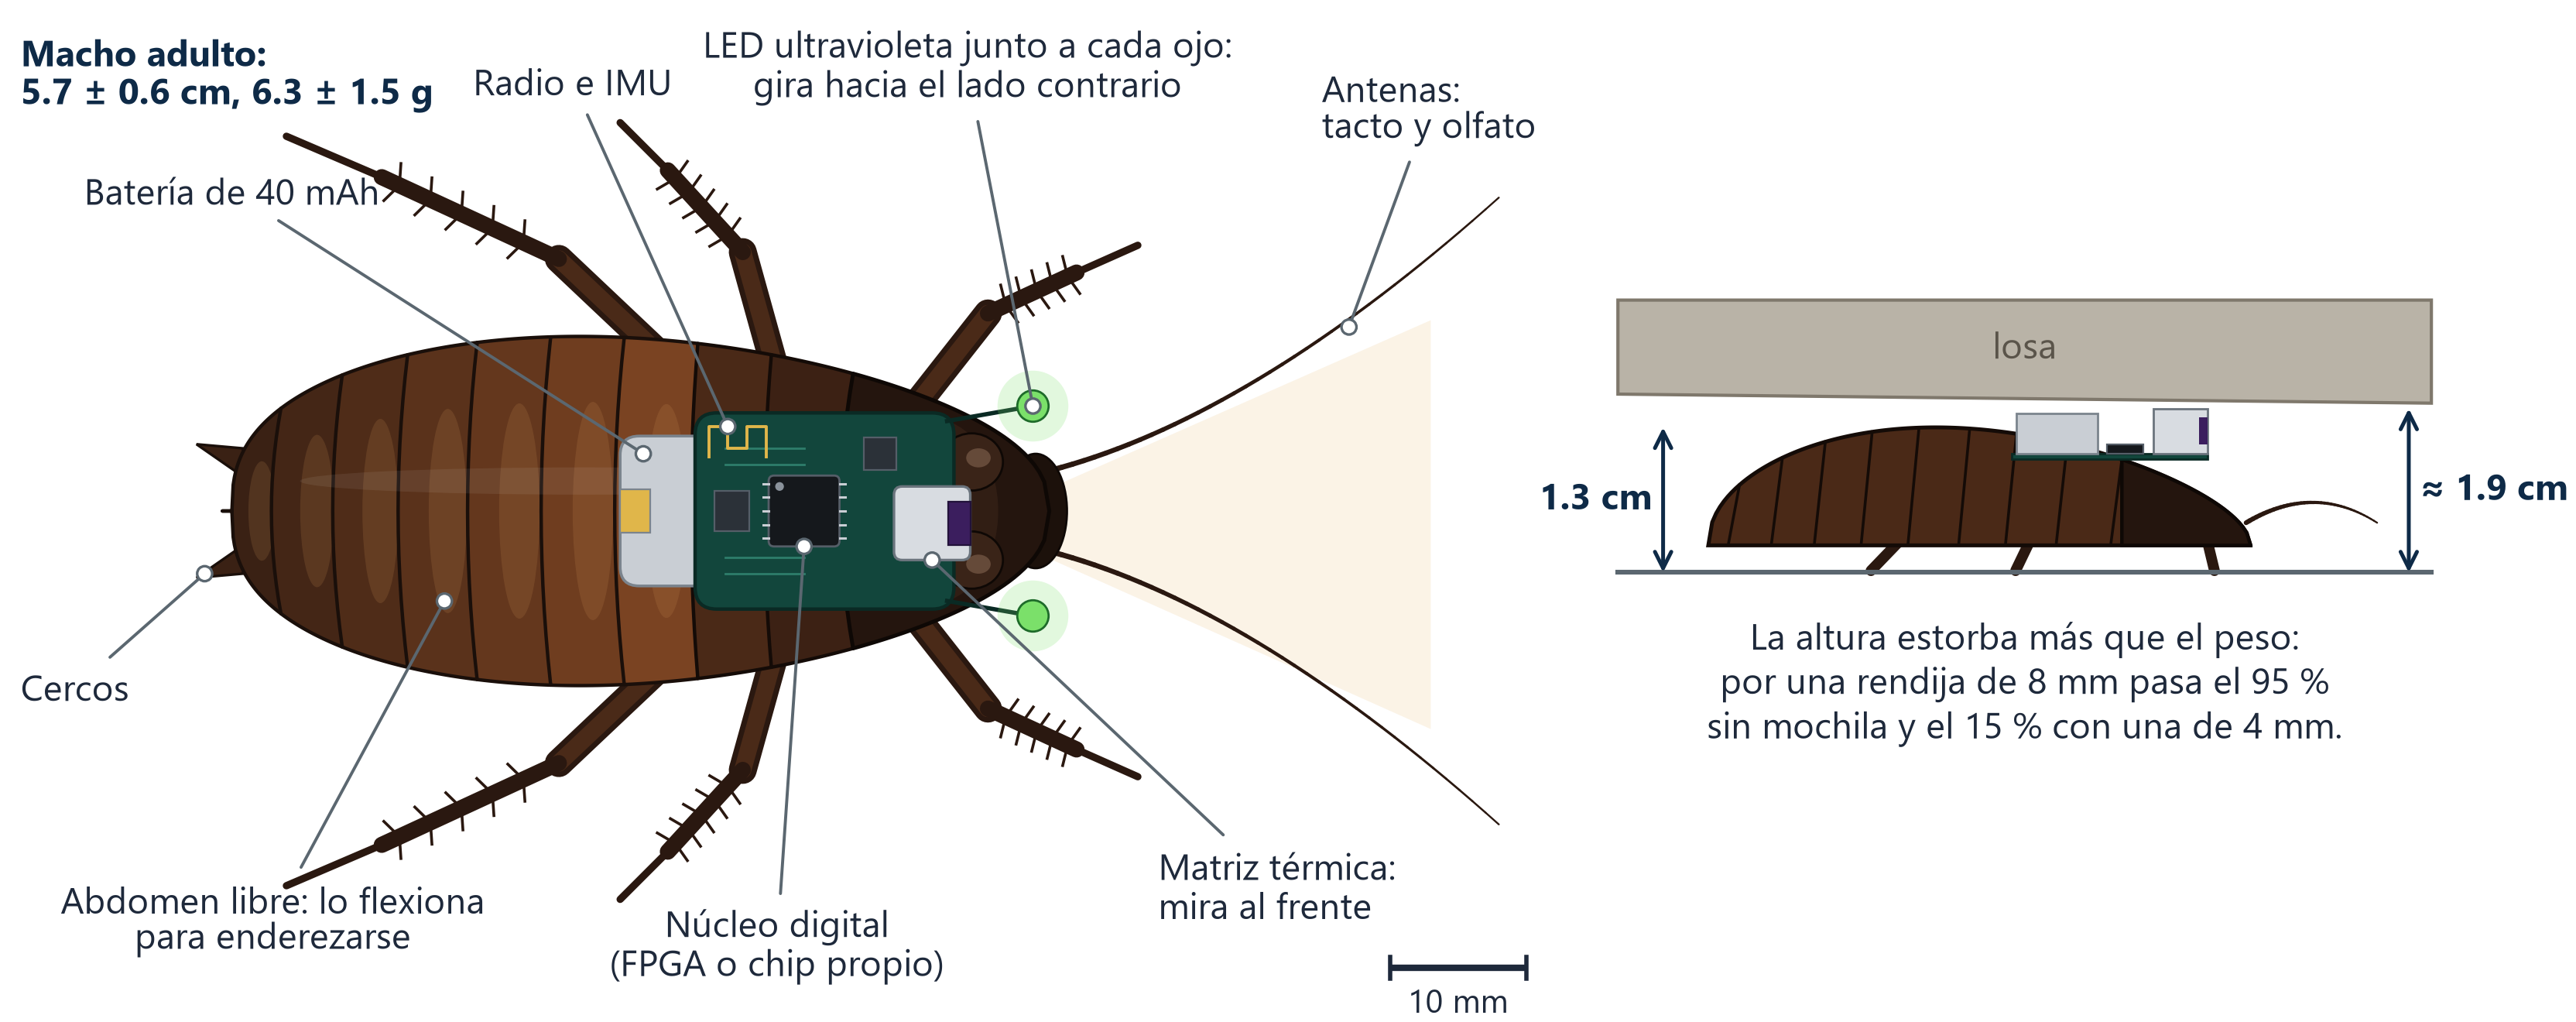
\includegraphics[width=\textwidth]{figs/insecto_mochila.png}
\caption{\Gp{} con la mochila, a escala. Dibujo esquemático propio; medidas de~\cite{tranngoc2023,li2019} y
paso por rendijas de~\cite{kai2026}.}
\label{fig:insecto}
\end{figure}

\begin{table}[H]
\centering\footnotesize
\caption{Capacidades de \Gp{} y lo que implican para la mochila.}
\label{tab:capacidades}
\rowcolors{2}{SoftGray}{white}
\begin{tabularx}{\textwidth}{@{}>{\bfseries\raggedright\arraybackslash}p{2.6cm} >{\raggedright\arraybackslash}p{5.4cm} >{\raggedright\arraybackslash}X@{}}
\toprule
\rowcolor{TableHead} Capacidad & Dato publicado & Consecuencia de diseño \\
\midrule
Masa y tamaño & Macho adulto: $6.32\pm1.5$~g y $5.7\pm0.6$~cm~\cite{tranngoc2023}; 2.2~cm de ancho y 1.3~cm de alto~\cite{li2019} & La mochila se dimensiona para un animal de 6~g \\
Carga & Se cita un máximo de 15~g, pero con 15~g se detiene por completo~\cite{montagut2024}; con 4~g ya empeora el control~\cite{latif2012} & Meta de 2 a 3~g (30 a 45~\% de la masa corporal) \\
Altura & Rendija de 8~mm: pasa el 95~\% sin mochila y el 15~\% con una de 4~mm~\cite{kai2026} & Componentes uno junto a otro, no apilados \\
Velocidad & 1.9~cm/s en marcha natural~\cite{dirafzoon2017}; 3.7 a 5.0~cm/s guiada~\cite{tranngoc2024}; 3.3~cm/s sostenida 20~min~\cite{herreid1981} & El modelo usa 1.9~cm/s y 5~cm/s durante 4~s tras un estímulo \\
Pausas & Sin estímulo pasa quieta cerca del 60~\% del tiempo, con pausas de 37~s en promedio~\cite{dirafzoon2017} & La política debe reiniciar la marcha \\
Obstáculos & Trepa un escalón de 1.5~cm en 48 de 49 intentos; no trepa una pared lisa de 10~cm: la bordea~\cite{tranngoc2023} & La exploración sigue contornos \\
Enderezarse & 98~\% sin carga; 31 a 69~\% con mochila y hasta 82~\% con un diseño que lo facilita~\cite{li2019,montagut2024} & Mochila baja y ligera; no pegar nada rígido en el abdomen~\cite{kakei2022} \\
Temperatura & Actividad máxima cerca de 30~\textdegree C; a 34 y 38~\textdegree C pasa inmóvil más de la mitad del tiempo~\cite{gracidas2026} & Ventana de operación de 22 a 30~\textdegree C \\
Sentidos & Sigue paredes y huye de la luz; no huye del viento~\cite{mcgorry2014}; nada indica que busque personas & La detección es tarea de la electrónica \\
Energía & 5~mW en reposo y 17 a 31~mW caminando (cálculo propio a partir de~\cite{herreid1981}) & La locomoción la paga el insecto; la mochila solo alimenta sensores y radio \\
Resistencia & Al menos un mes sin comida ni agua~\cite{yoder1997}; vive de 2 a 5 años; no vuela ni muerde & Logística sencilla: se cría y se transporta sin cuidados especiales \\
\bottomrule
\end{tabularx}
\end{table}

\begin{figure}[H]
\centering
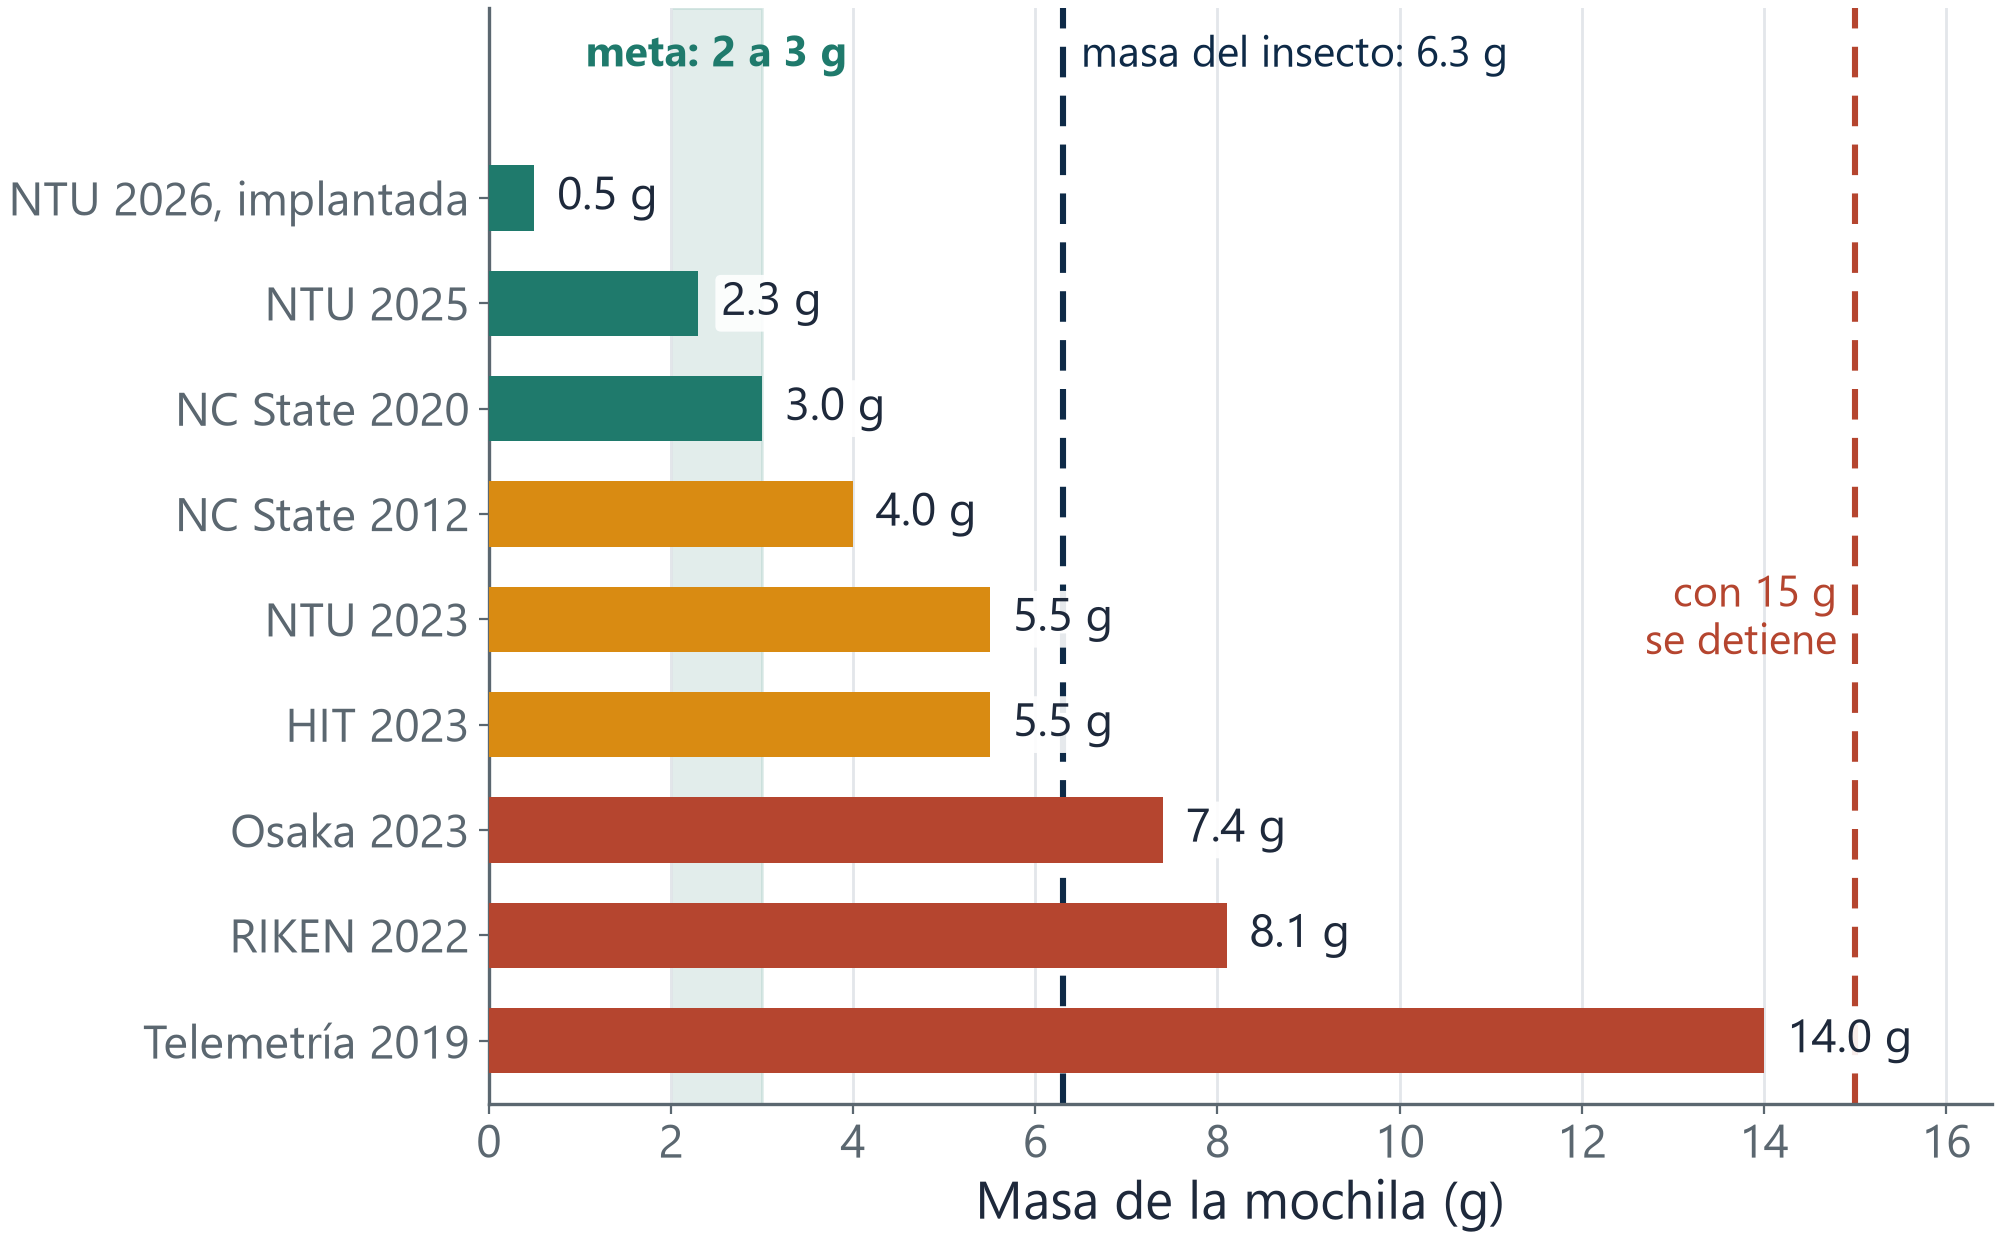
\includegraphics[width=0.78\textwidth]{figs/mochilas_publicadas.png}
\caption{Masa de las mochilas publicadas para esta especie. La tendencia es bajar masa y perfil:
el grupo de NTU pasó de 5.5~g en 2023 a 2.3~g en 2025 y a un controlador implantado de 0.5~g en 2026.}
\label{fig:mochilas}
\end{figure}

\subsection*{Supuestos iniciales que se corrigen}

La revisión obligó a cambiar cuatro cifras con las que arrancó el proyecto
(tabla~\ref{tab:correcciones}).

\begin{table}[H]
\centering\footnotesize
\caption{Supuestos de la propuesta inicial frente a la evidencia.}
\label{tab:correcciones}
\rowcolors{2}{SoftGray}{white}
\begin{tabularx}{\textwidth}{@{}>{\bfseries\raggedright\arraybackslash}p{3.1cm} >{\raggedright\arraybackslash}p{3.6cm} >{\raggedright\arraybackslash}X@{}}
\toprule
\rowcolor{TableHead} Supuesto inicial & Valor inicial & Evidencia y valor adoptado \\
\midrule
Carga útil & 15~g sin afectar la marcha & 15~g es el punto en que el insecto se detiene~\cite{montagut2024}. Se adoptan 2 a 3~g \\
Velocidad & 0.3~m/s & Lo medido va de 3 a 9~cm/s; 0.3~m/s corresponde a otras especies. Se adoptan 1.9 y 5~cm/s \\
Detección térmica & Umbral fijo de 35.5 a 38.5~\textdegree C & Es temperatura central; la piel expuesta está entre 27 y 35~\textdegree C y el sensor promedia su campo de visión. Se cuenta píxeles calientes sobre el fondo \\
Tamaño del circuito & Menos de 60 celdas & La síntesis del núcleo completo da 224 registros y 477 elementos lógicos \\
\bottomrule
\end{tabularx}
\end{table}

\section{El modelo}

El modelo encadena cinco partes (figura~\ref{fig:marco}). Cada una entrega a la siguiente un
número con el que se puede diseñar, y todas quedan acotadas por la capa ética y normativa de
la sección~\ref{sec:etica}.

\begin{figure}[H]
\centering
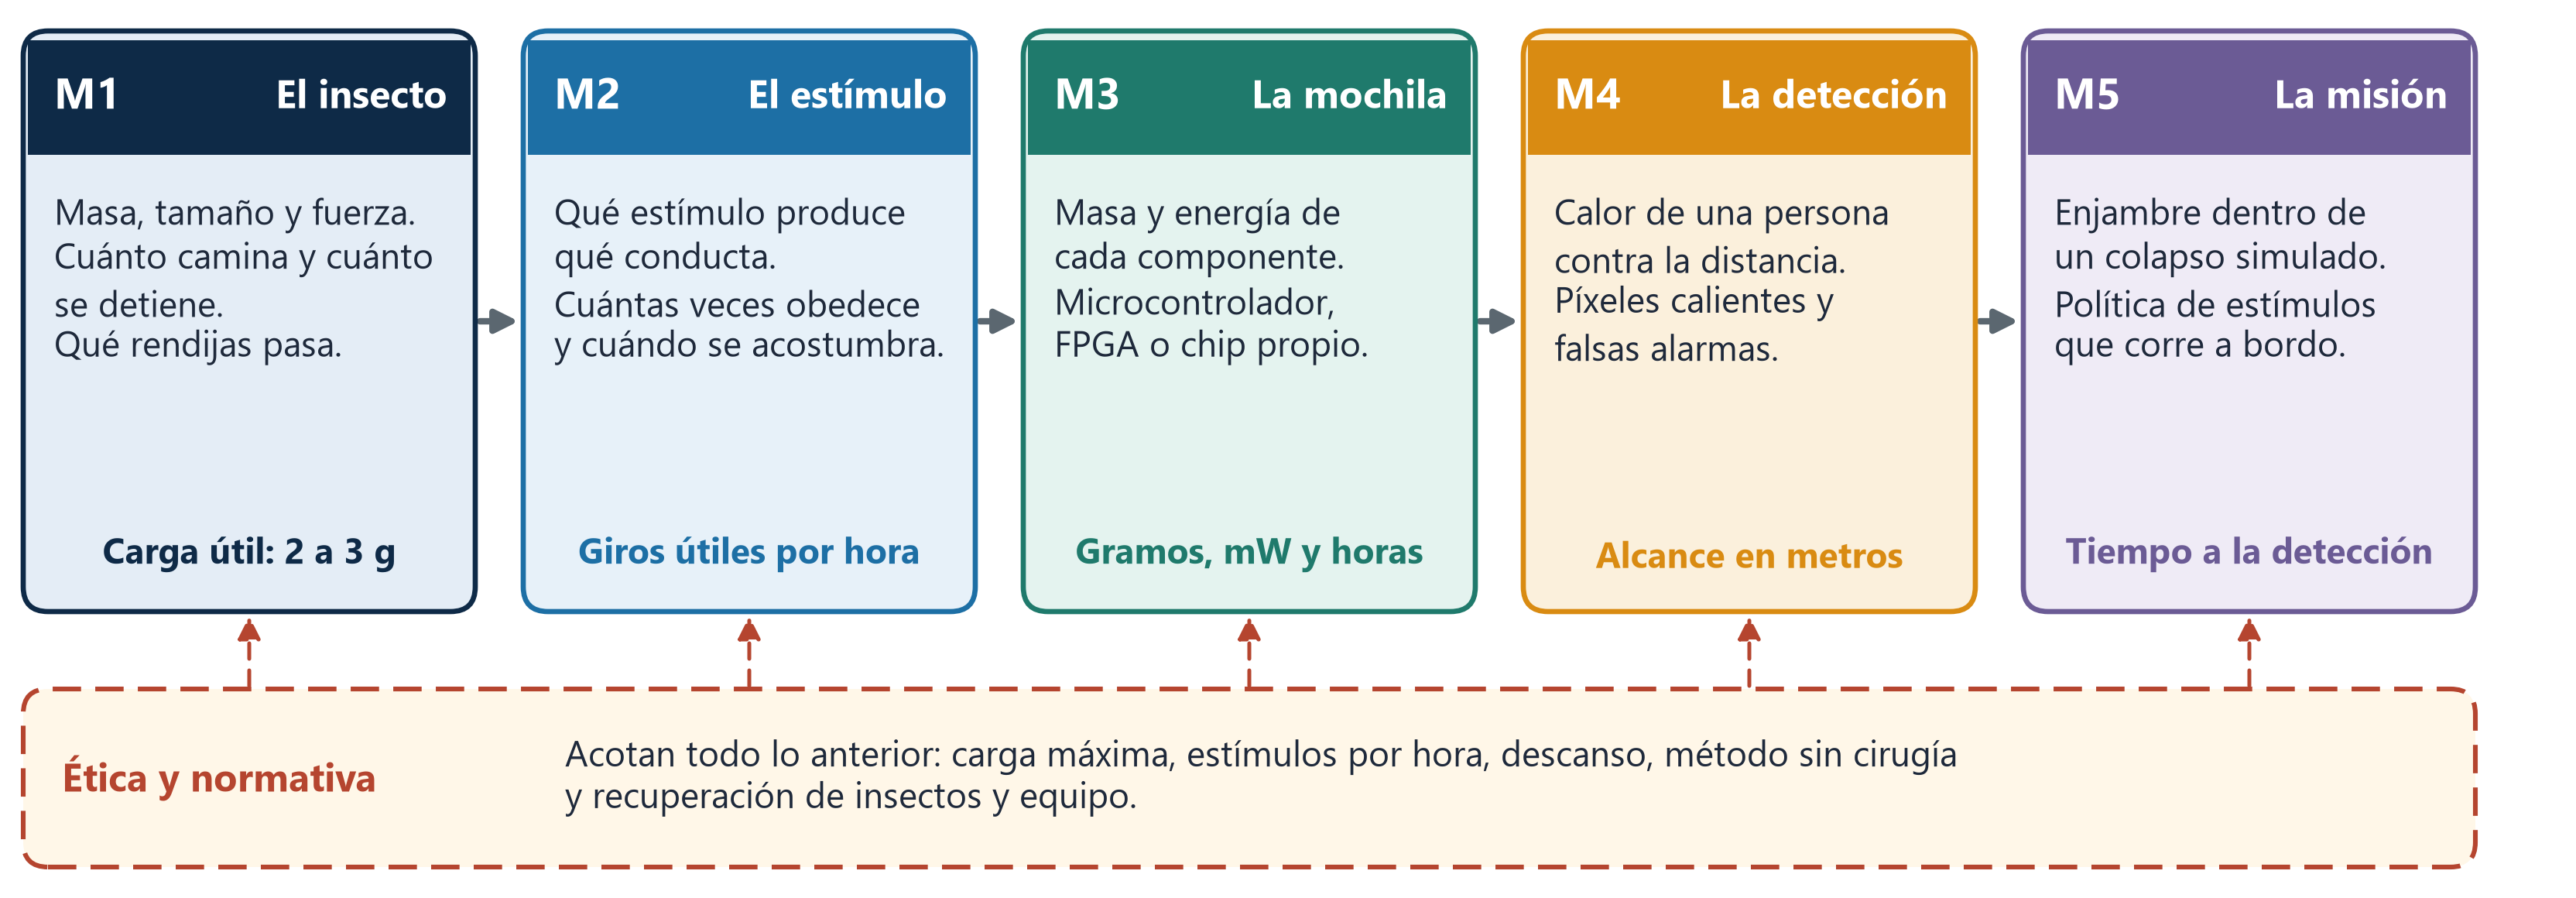
\includegraphics[width=\textwidth]{figs/marco_modelo.png}
\caption{Marco del modelo: cinco submodelos encadenados y la capa que los acota.}
\label{fig:marco}
\end{figure}

\subsection{M1. El insecto: marcha natural}

La marcha sin estímulo se describe con el modelo de Dirafzoon et al.~\cite{dirafzoon2017}, con
los valores que usan Tran-Ngoc et al.~\cite{tranngoc2024}. El insecto camina tramos rectos de
longitud exponencial con media $l^*=17.6$~cm a $v=1.94$~cm/s. Al terminar cada tramo se
detiene con probabilidad $P_s=0.211$ durante un tiempo de media $T_s=36.8$~s; si no se detiene,
gira un ángulo pequeño. Cuando toca una pared la sigue, y solo la suelta con probabilidad
$p_e=0.005$ por tramo. De ahí sale la fracción del tiempo que pasa caminando:
\begin{equation}
F_m=\frac{l^*/v}{l^*/v+P_s\,T_s}=\frac{9.1}{9.1+7.8}=0.54 ,
\end{equation}
dentro del intervalo medido de $0.37\pm0.20$. La carga útil y la altura salen de la
tabla~\ref{tab:capacidades}: $m_c\le3$~g y componentes no apilados.

\subsection{M2. El estímulo}

\begin{table}[H]
\centering\footnotesize
\caption{Tipos de estímulo para dirigir a \Gp.}
\label{tab:estimulos}
\rowcolors{2}{SoftGray}{white}
\begin{tabularx}{\textwidth}{@{}>{\bfseries\raggedright\arraybackslash}p{2.7cm} >{\raggedright\arraybackslash}p{1.5cm} >{\raggedright\arraybackslash}p{3.0cm} >{\raggedright\arraybackslash}p{3.3cm} >{\raggedright\arraybackslash}X@{}}
\toprule
\rowcolor{TableHead} Estímulo & Cirugía & Conducta & Eficacia publicada & Inconveniente \\
\midrule
Electrodo implantado en la antena~\cite{latif2012,erickson2015} & Sí & Giro al lado contrario & 56~\% de los individuos; giros con mediana de 130\textdegree & Inutiliza la antena; el implante dura días \\
Electrodo implantado en los cercos~\cite{tranngoc2023} & Sí & Avance; giro con un solo cerco & 94~\% de navegaciones & Las fuentes no coinciden en el sentido del giro \\
Electrodo torácico~\cite{lin2025} & Poca & Giro y freno & Giro de más de 70\textdegree{} en 0.4~s & Requiere ensamble preciso \\
Electrodo de superficie en antena y abdomen~\cite{lin2023,tranngoc2025} & No & Giro y avance & 81~\% y 74~\% por estímulo; giro medio de 38\textdegree & Impedancia alta: 70 a 123~k$\Omega$ \\
Luz ultravioleta junto a los ojos~\cite{refat2025,gracidas2026} & No & Giro al lado contrario; reanuda la marcha & Sin habituación en 150 ensayos; aumenta la locomoción & Falta medir el ángulo por pulso \\
Calor en los tarsos & No & Escape & Cualitativa & Unos 330~mW por estímulo~\cite{erickson2015}: 100 veces el eléctrico \\
\bottomrule
\end{tabularx}
\end{table}

Todos los estímulos eléctricos usan una onda cuadrada bifásica de 40 a 55~Hz, con ciclo de
trabajo de 50~\% y trenes de 0.4 a 1~s; con electrodo implantado bastan 2 a 3~V, y subir el
voltaje empeora la respuesta~\cite{erickson2015,lin2025}. El tren cuesta unos 2.2~mW mientras
dura~\cite{erickson2015}, así que el estímulo no pesa en la energía.

\textbf{Elección.} Se adopta la luz ultravioleta como estímulo principal, porque no requiere
cirugía, no se ha observado habituación y la misma colonia de la universidad responde a
ella~\cite{gracidas2026}; los electrodos de superficie quedan como alternativa. El generador
de pulsos del núcleo sirve para los dos casos.

\textbf{Respuesta y habituación.} El insecto obedece un estímulo con probabilidad
$p\,(1-H)$, donde $p=0.78$~\cite{lin2023} y $H$ es la habituación. Cada estímulo la sube y el
descanso la baja:
\begin{equation}
H\leftarrow H+\alpha\,(1-H) \quad\text{por estímulo},\qquad
H(t+\Delta t)=H(t)\,e^{-\Delta t/\tau}.
\end{equation}
Con $\tau=600$~s (las fuentes dan de 5 a 20~min de recuperación~\cite{sanchez2015}) y
$\alpha=0.09$, el modelo reproduce los tres datos disponibles para pulsos unipolares: queda el
46~\% de la respuesta tras diez estímulos cada 15~s (medido: 43~\%~\cite{ma2023}), el 71~\% cada
120~s (medido: 66~\%) y el 22~\% tras cuarenta ensayos (medido: 20~\%~\cite{erickson2015}). Con
onda bifásica o con luz, $\alpha$ es al menos cuarenta veces menor (figura~\ref{fig:habituacion}).
La simulación usa $\alpha=0.01$, un valor conservador.

\begin{figure}[H]
\centering
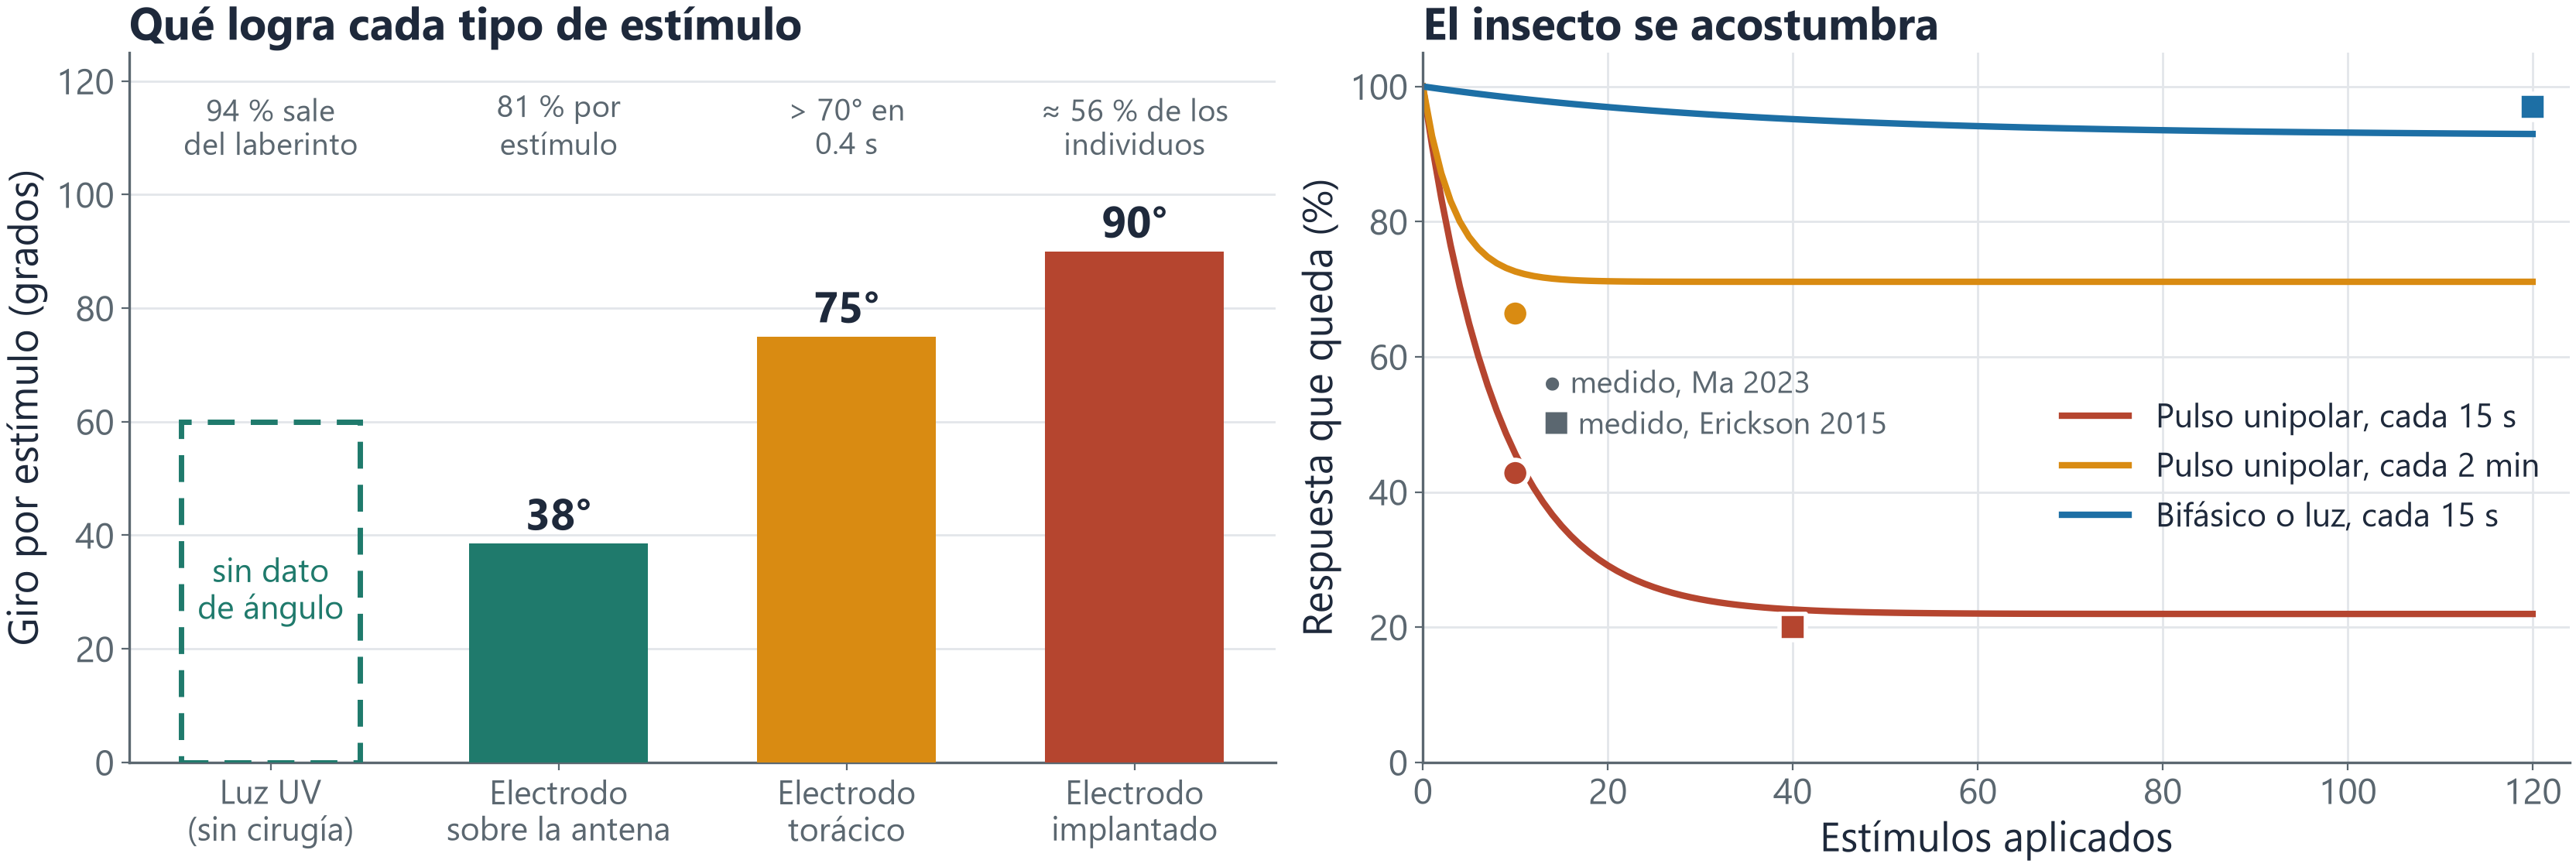
\includegraphics[width=\textwidth]{figs/habituacion.png}
\caption{Izquierda: giro por estímulo según el método~\cite{lin2023,lin2025,ma2023}. Derecha: modelo de
habituación frente a los datos medidos.}
\label{fig:habituacion}
\end{figure}

\subsection{M3. La mochila: masa, energía y cómputo}

\begin{figure}[H]
\centering
\begin{subfigure}{0.49\textwidth}
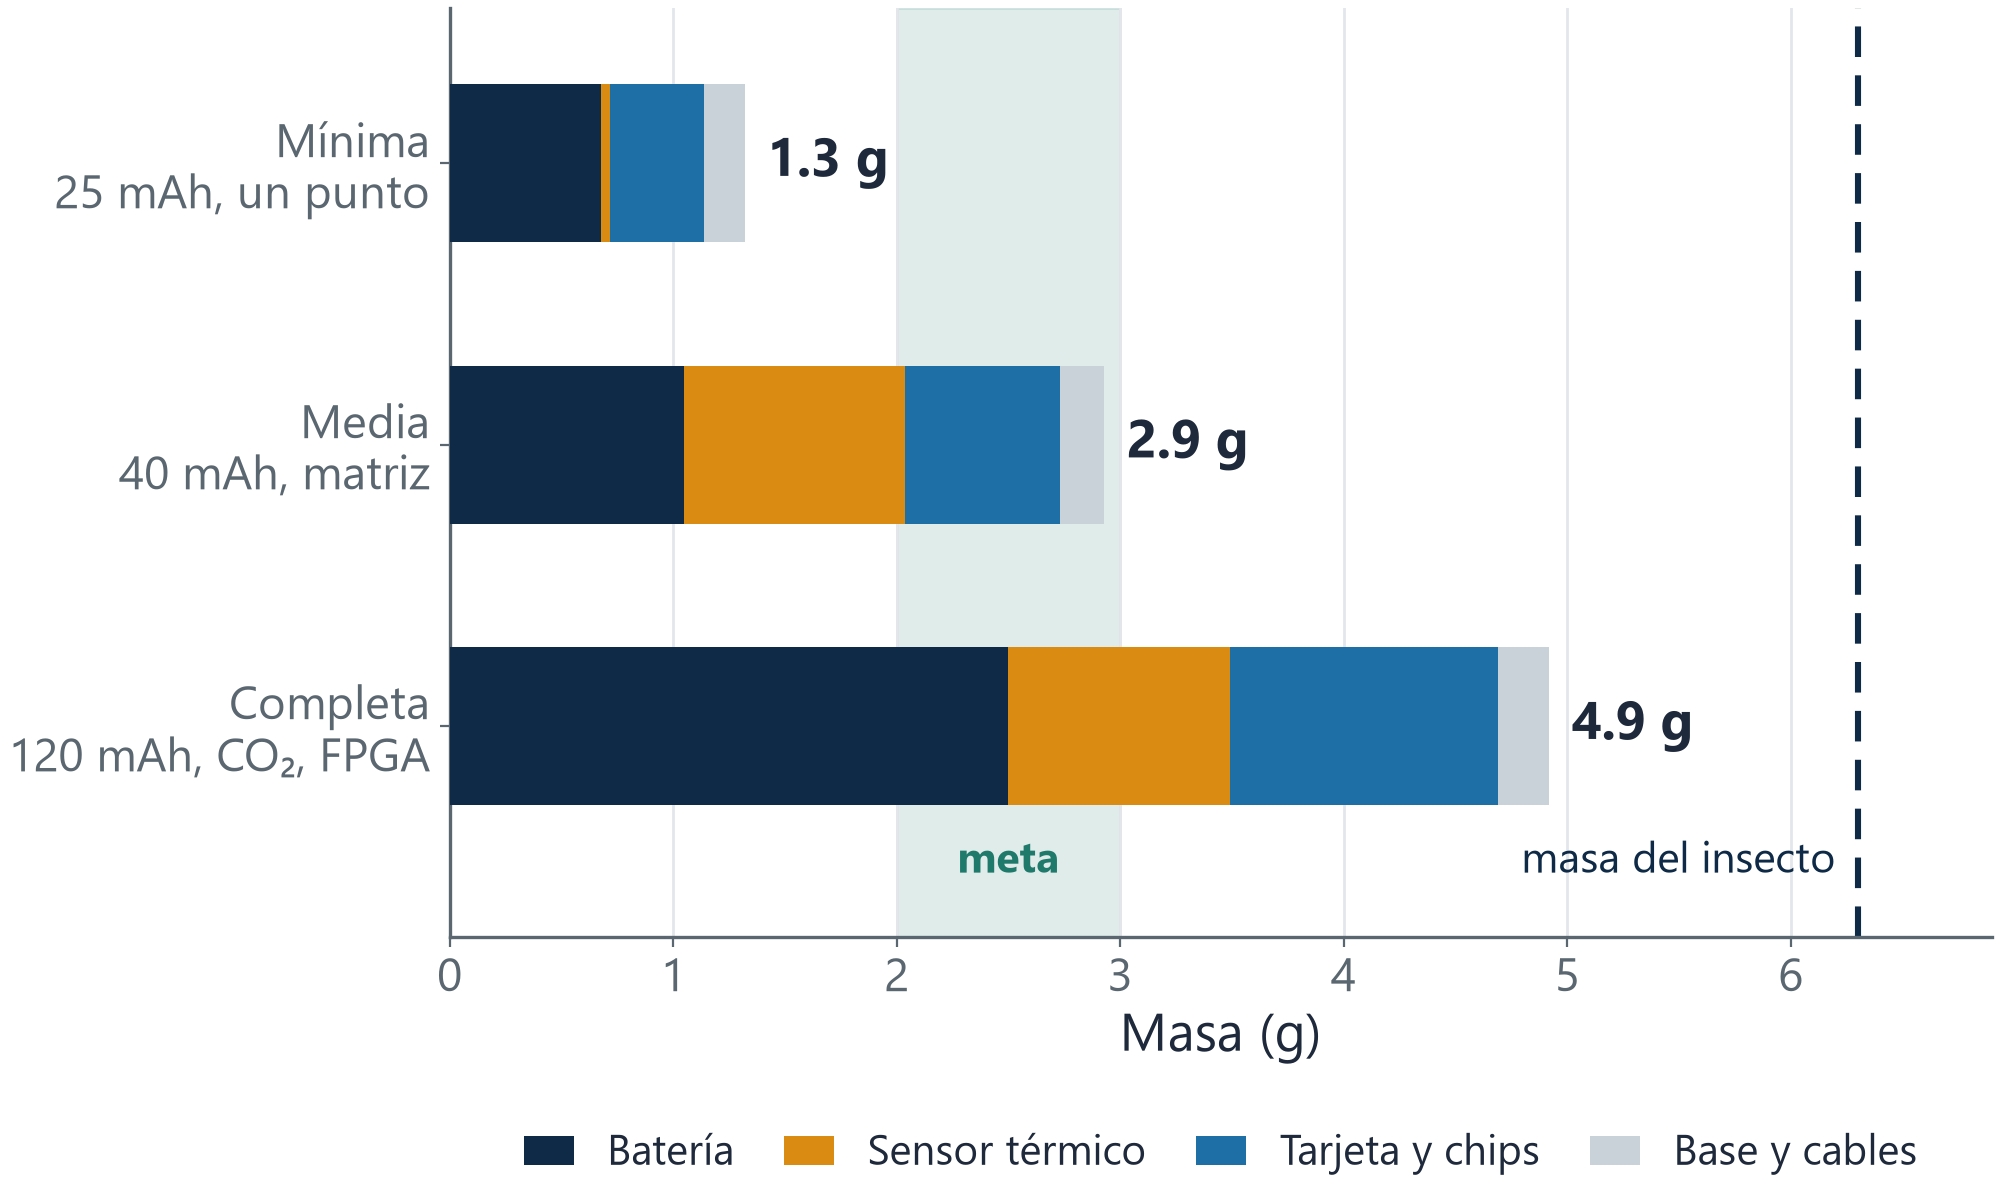
\includegraphics[width=\linewidth]{figs/presupuesto_masa.png}
\caption{Masa por configuración.}
\end{subfigure}\hfill
\begin{subfigure}{0.49\textwidth}
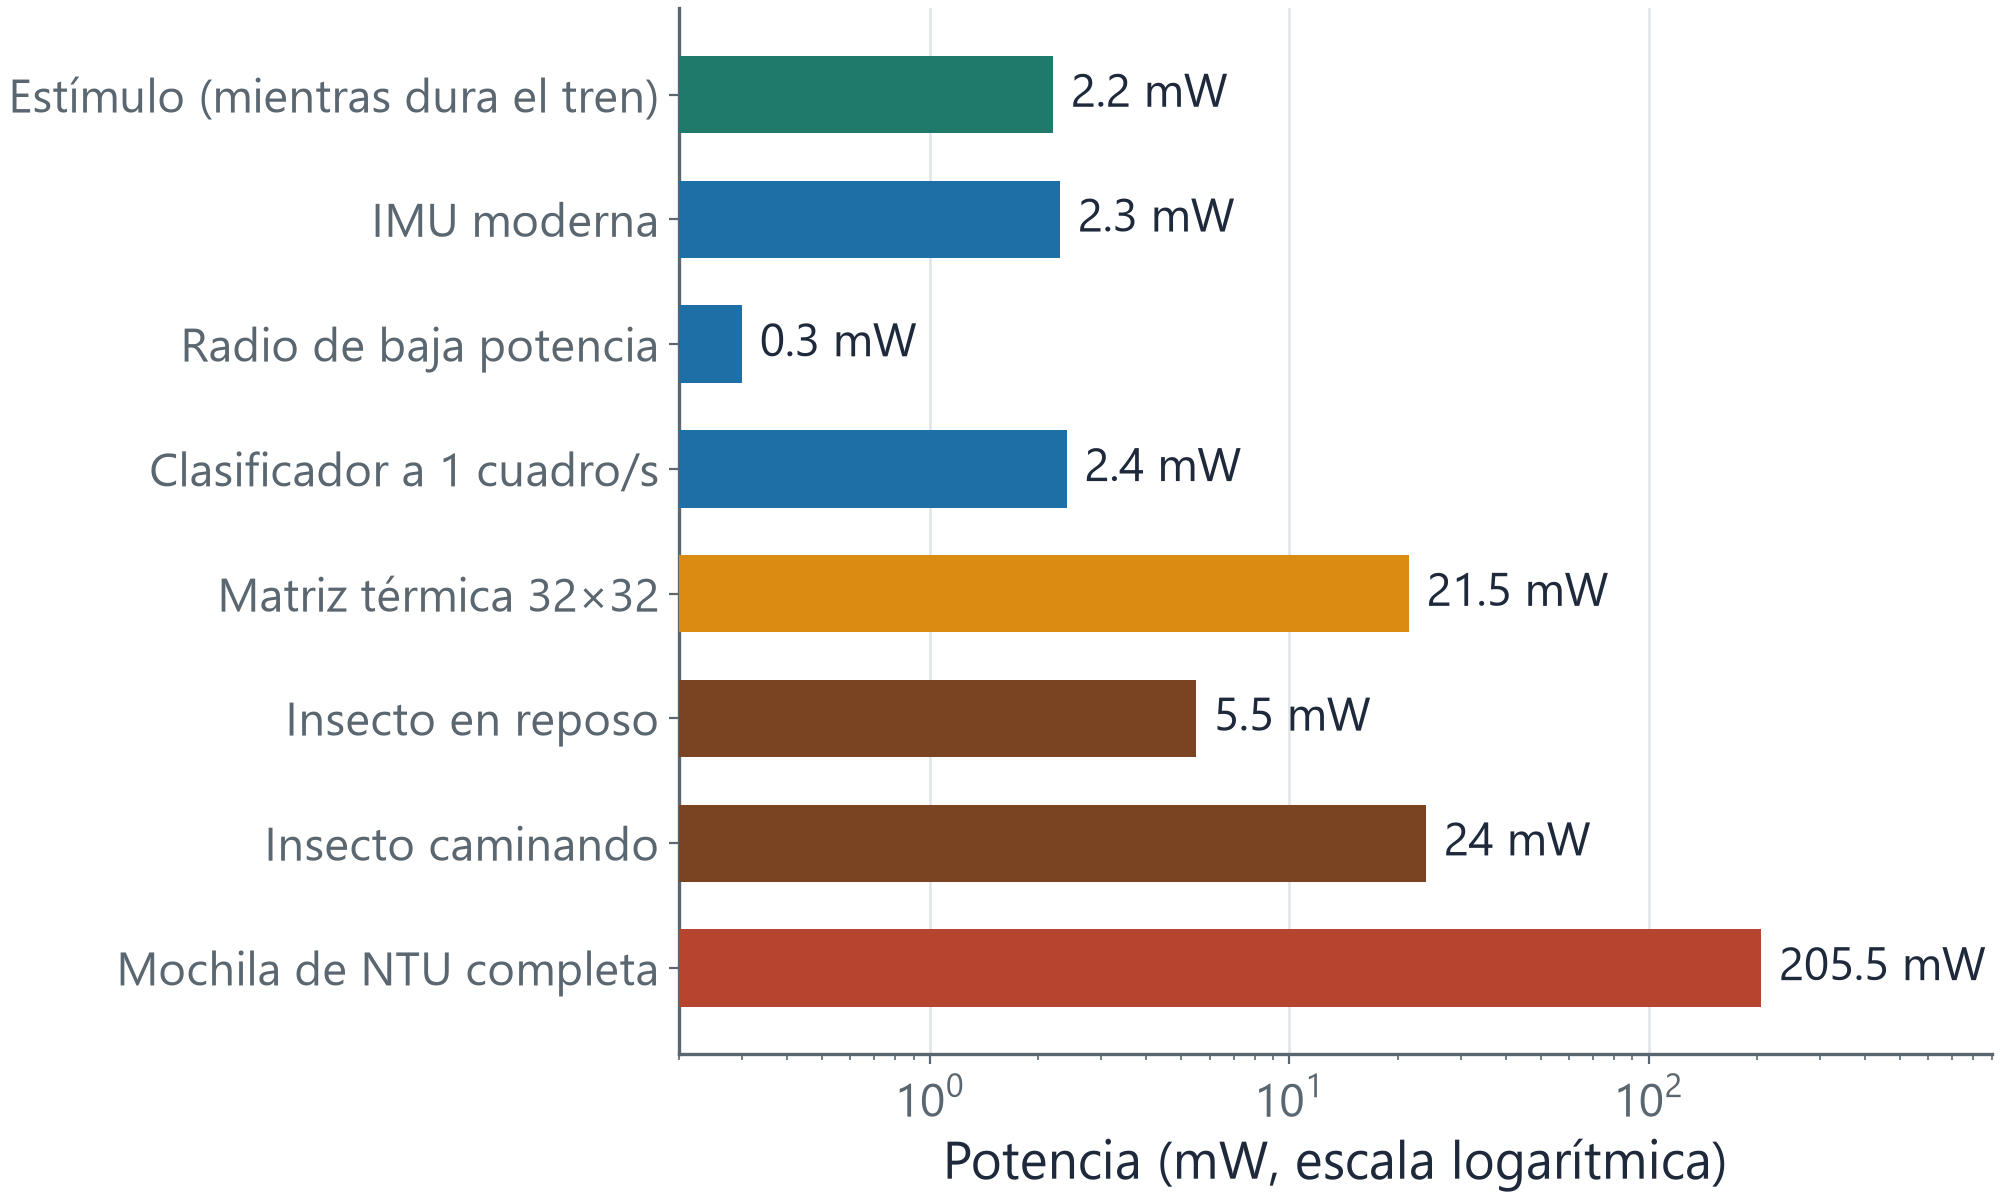
\includegraphics[width=\linewidth]{figs/energia.png}
\caption{Quién gasta qué.}
\end{subfigure}
\caption{Presupuestos de la mochila. La batería y el sensor térmico mandan en la masa; el sensor manda
en la energía. Masas de batería y sensor medidas~\cite{tranngoc2023}; las de los chips son estimadas.}
\label{fig:presupuestos}
\end{figure}

Se adopta la configuración media: matriz térmica, radio de baja potencia, IMU y una batería de
40~mAh, unos 2.9~g. Con el sensor encendido todo el tiempo consume cerca de 30~mW y la
autonomía estimada es
\begin{equation}
t=\frac{0.85\times40~\text{mAh}\times3.7~\text{V}}{30~\text{mW}}\approx4~\text{h},
\end{equation}
que sube a unas 10~h si el sensor trabaja la cuarta parte del tiempo. Como referencia medida,
la mochila de NTU consume 205.5~mW y dura 2.2~h con 120~mAh~\cite{tranngoc2023}.

\textbf{Relación entre carga y capacidad de cómputo.} El cómputo casi no pesa
(tabla~\ref{tab:computo}): una FPGA de 1\,248 LUT cabe en 2~mm$^2$. Lo que el insecto no
puede cargar son baterías grandes ni sensores altos. Por eso conviene gastar lógica, que es
gratis en masa, para ahorrar energía y estímulos.

\begin{table}[H]
\centering\footnotesize
\caption{Qué cómputo cabe en la mochila. Masas estimadas a partir del encapsulado.}
\label{tab:computo}
\rowcolors{2}{SoftGray}{white}
\begin{tabularx}{\textwidth}{@{}>{\bfseries\raggedright\arraybackslash}p{3.7cm} >{\raggedright\arraybackslash}p{2.6cm} >{\raggedright\arraybackslash}p{1.6cm} >{\raggedright\arraybackslash}p{2.2cm} >{\raggedright\arraybackslash}X@{}}
\toprule
\rowcolor{TableHead} Dispositivo & Tamaño & Masa & Reposo & Capacidad \\
\midrule
nRF52840 (radio y procesador)~\cite{nordic} & $3.5\times3.6$~mm & $\approx15$~mg & 0.4~$\mu$A & Cortex-M4, 1~MB; transmite con 6.4~mA \\
iCE40 UltraLite UL1K~\cite{lattice} & $1.4\times1.4$~mm & $\approx2$~mg & 35~$\mu$A & 1\,248 LUT: aloja el núcleo (477) \\
iCE40 UltraPlus UP5K~\cite{lattice} & $2.15\times2.55$~mm & $\approx6$~mg & 75~$\mu$A & 5\,280 LUT, 8 multiplicadores \\
Chip propio en SKY130~\cite{tinytapeout} & $160\times100~\mu$m por módulo & $<1$~mg & Por medir & Unas 1\,000 compuertas por módulo \\
Tarjeta de desarrollo (XIAO, SuperMini) & $21\times18$~mm & 1.5 a 2.5~g & 44~$\mu$A o más & Solo para la maqueta: consume la carga útil \\
\bottomrule
\end{tabularx}
\end{table}

\subsection{M4. La detección}
\label{sec:deteccion}

Un sensor térmico de un solo píxel promedia todo su campo de visión. Si el blanco tiene área
$A$ y está a distancia $d$, solo llena una fracción $f$ del campo, y la lectura es
\begin{equation}
T_{\text{leída}}=T_f+f\,(T_p-T_f),\qquad
f=\min\!\left(1,\ \frac{A}{\pi\,d^2\tan^2(\varphi/2)}\right).
\end{equation}
Con una cara ($A=0.03$~m$^2$), piel a 33~\textdegree C, fondo a 22~\textdegree C y campo de
$\varphi=90$\textdegree, a medio metro la lectura es de 22.4~\textdegree C. Un umbral fijo de
35.5 a 38.5~\textdegree C no se alcanza ni pegado a la persona, porque ese intervalo es de
temperatura central y la piel expuesta está entre 27 y 35~\textdegree C.

Una matriz resuelve el problema, porque cada píxel ve un ángulo pequeño $\theta$ y el blanco
ocupa
\begin{equation}
n=\frac{A}{(d\tan\theta)^2}\quad\text{píxeles}.
\end{equation}
El núcleo cuenta como caliente todo píxel que esté entre 28 y 38~\textdegree C, el criterio de
NTU~\cite{tranngoc2023}, \emph{y además} 2~\textdegree C por encima de la media del cuadro
anterior, para que un ambiente tibio no llene la imagen. Con 2 píxeles empieza a acercarse y
con 8 durante cuatro cuadros seguidos declara la detección (figura~\ref{fig:deteccion}).

\begin{figure}[H]
\centering
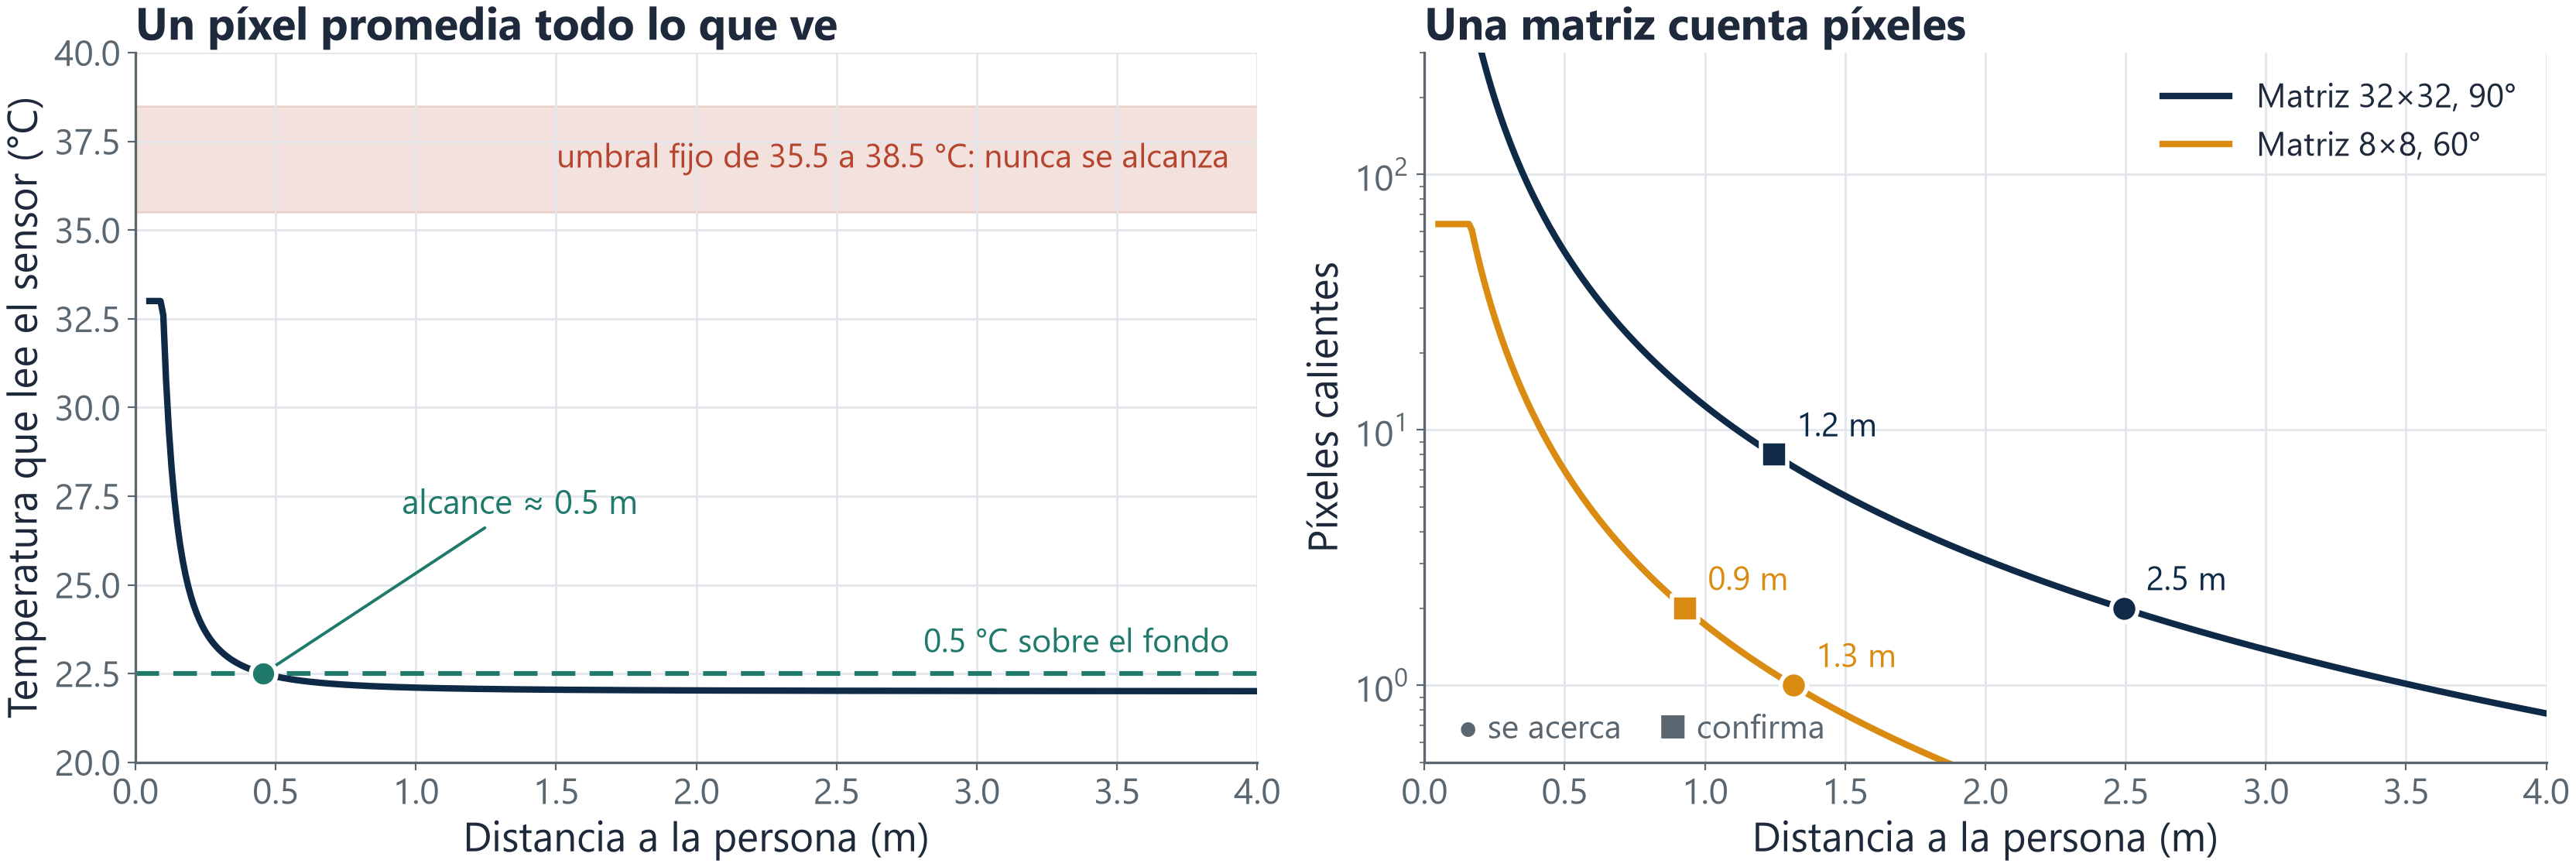
\includegraphics[width=\textwidth]{figs/deteccion_termica.png}
\caption{Izquierda: lectura de un píxel de 90\textdegree{} frente a la distancia. Derecha: píxeles calientes
con dos matrices; el círculo marca dónde empieza el acercamiento y el cuadro dónde se confirma.}
\label{fig:deteccion}
\end{figure}

\begin{table}[H]
\centering\footnotesize
\caption{Sensores térmicos candidatos. Precios de mostrador en México al 9 de noviembre de 2026~\cite{unit}.}
\label{tab:sensores}
\rowcolors{2}{SoftGray}{white}
\begin{tabularx}{\textwidth}{@{}>{\bfseries\raggedright\arraybackslash}p{3.4cm} >{\raggedright\arraybackslash}p{2.0cm} >{\raggedright\arraybackslash}p{1.9cm} >{\raggedright\arraybackslash}p{2.6cm} >{\raggedright\arraybackslash}X@{}}
\toprule
\rowcolor{TableHead} Sensor & Píxeles y campo & Consumo & Alcance (acercar / confirmar) & Precio \\
\midrule
MLX90614 (un punto)~\cite{melexis} & 1; 90\textdegree & Sin verificar & 0.6 / 0.4~m & 189~MXN \\
AMG8833~\cite{panasonic} & $8\times8$; 60\textdegree & 4.5~mA & 1.3 / 0.9~m & 599~MXN \\
MLX90640~\cite{melexis} & $32\times24$; 55\textdegree & $<23$~mA & 4.1 / 2.0~m & 1\,100~MXN \\
Heimann HTPA32x32d~\cite{tranngoc2023} & $32\times32$; 90\textdegree & 6.5~mA & 2.5 / 1.2~m & Sin precio local \\
\bottomrule
\end{tabularx}
\end{table}

\textbf{Límites de la detección térmica.} Si el ambiente pasa de unos 30~\textdegree C, el
contraste con la piel se pierde: en Myanmar el ambiente rondaba los 38~\textdegree C. A esa
temperatura, además, el insecto pasa inmóvil más de la mitad del tiempo~\cite{gracidas2026}
(figura~\ref{fig:ventana}). El CO$_2$ exhalado, que llega a 1.6~\% en un hueco
cerrado~\cite{huo2011}, y el sonido son las señales complementarias; quedan como trabajo
futuro porque los sensores de CO$_2$ pequeños responden en 20 a 60~s.

\begin{figure}[H]
\centering
\begin{subfigure}{0.49\textwidth}
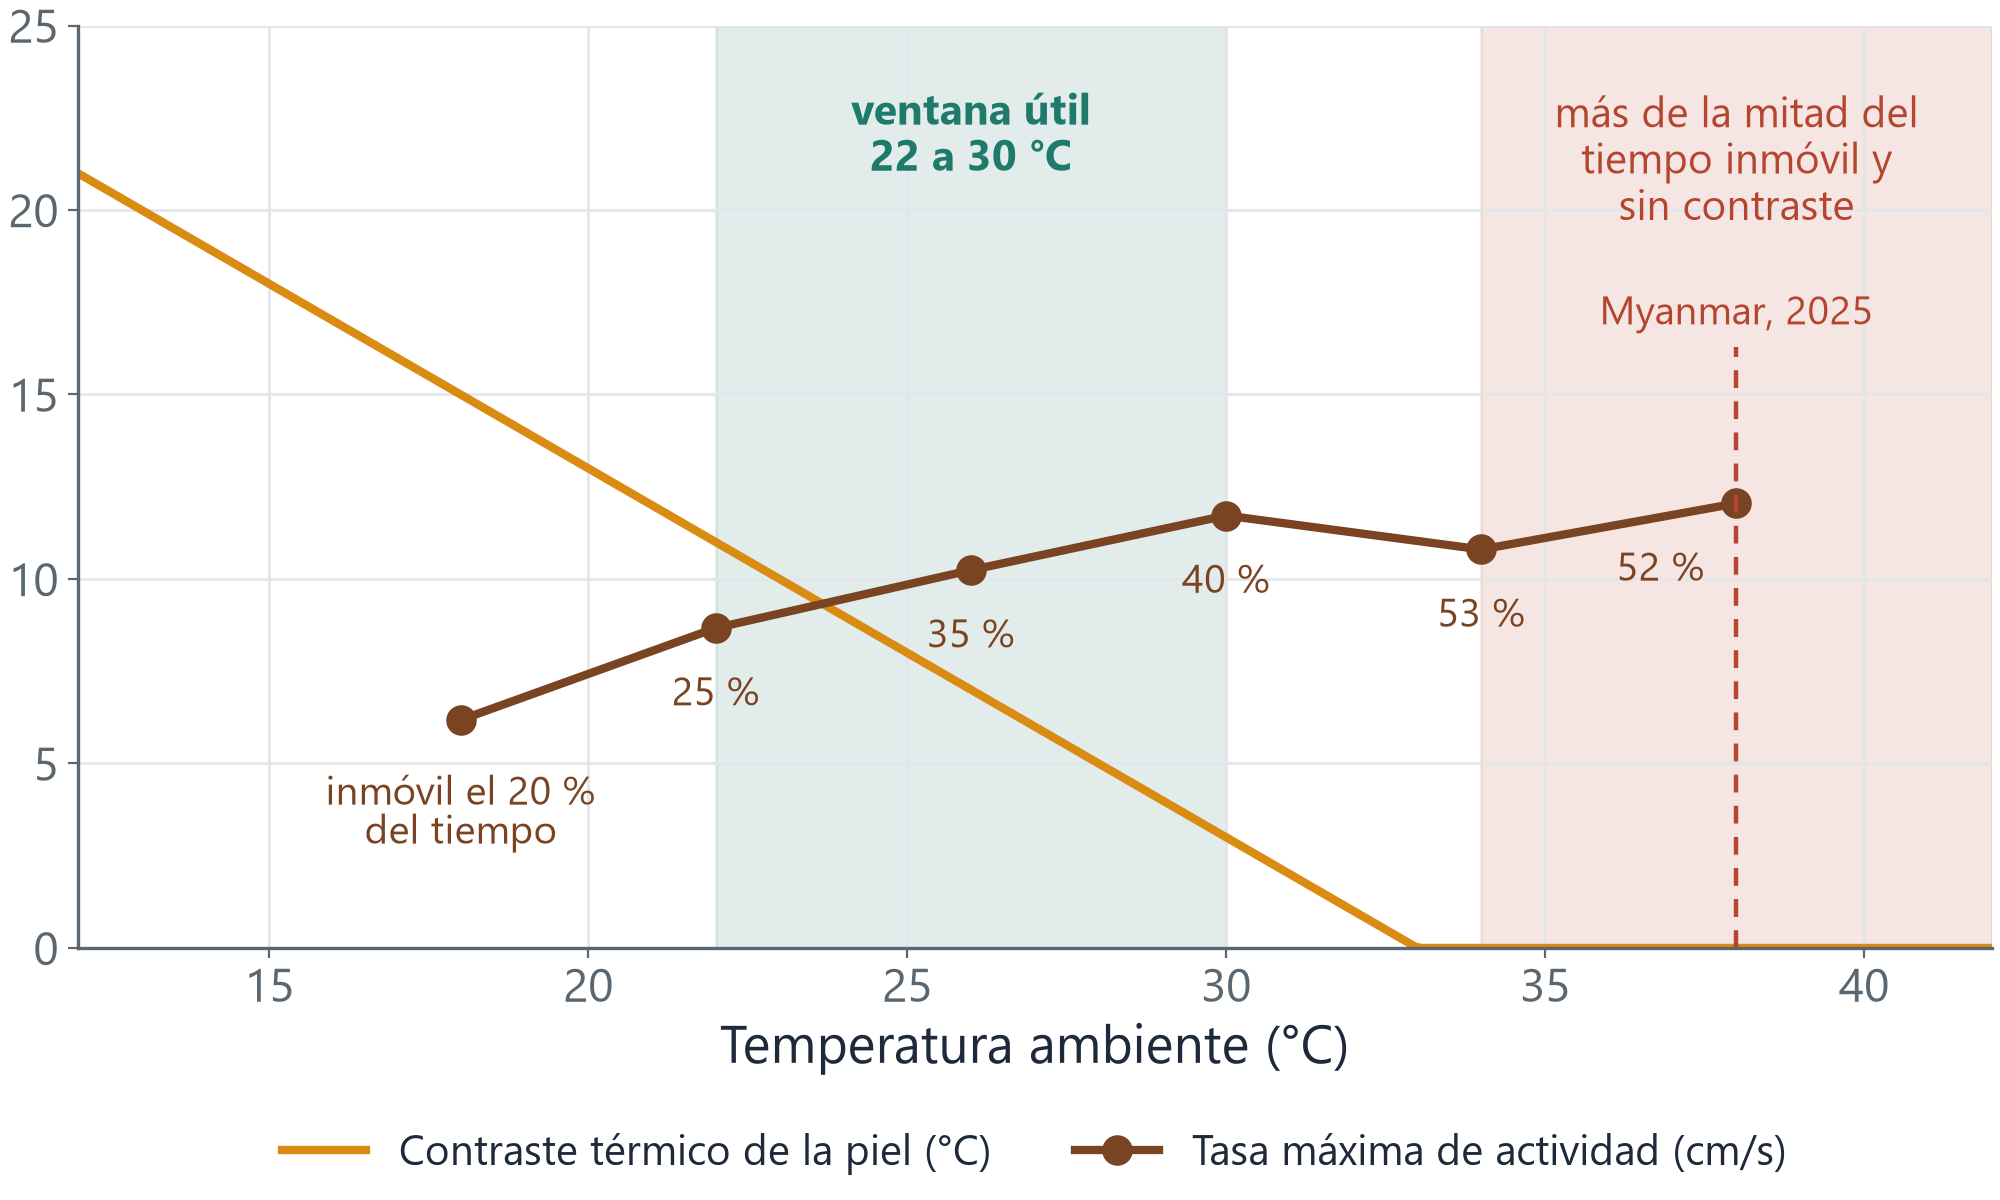
\includegraphics[width=\linewidth]{figs/ventana_operativa.png}
\caption{Ventana de temperatura.}
\label{fig:ventana}
\end{subfigure}\hfill
\begin{subfigure}{0.49\textwidth}
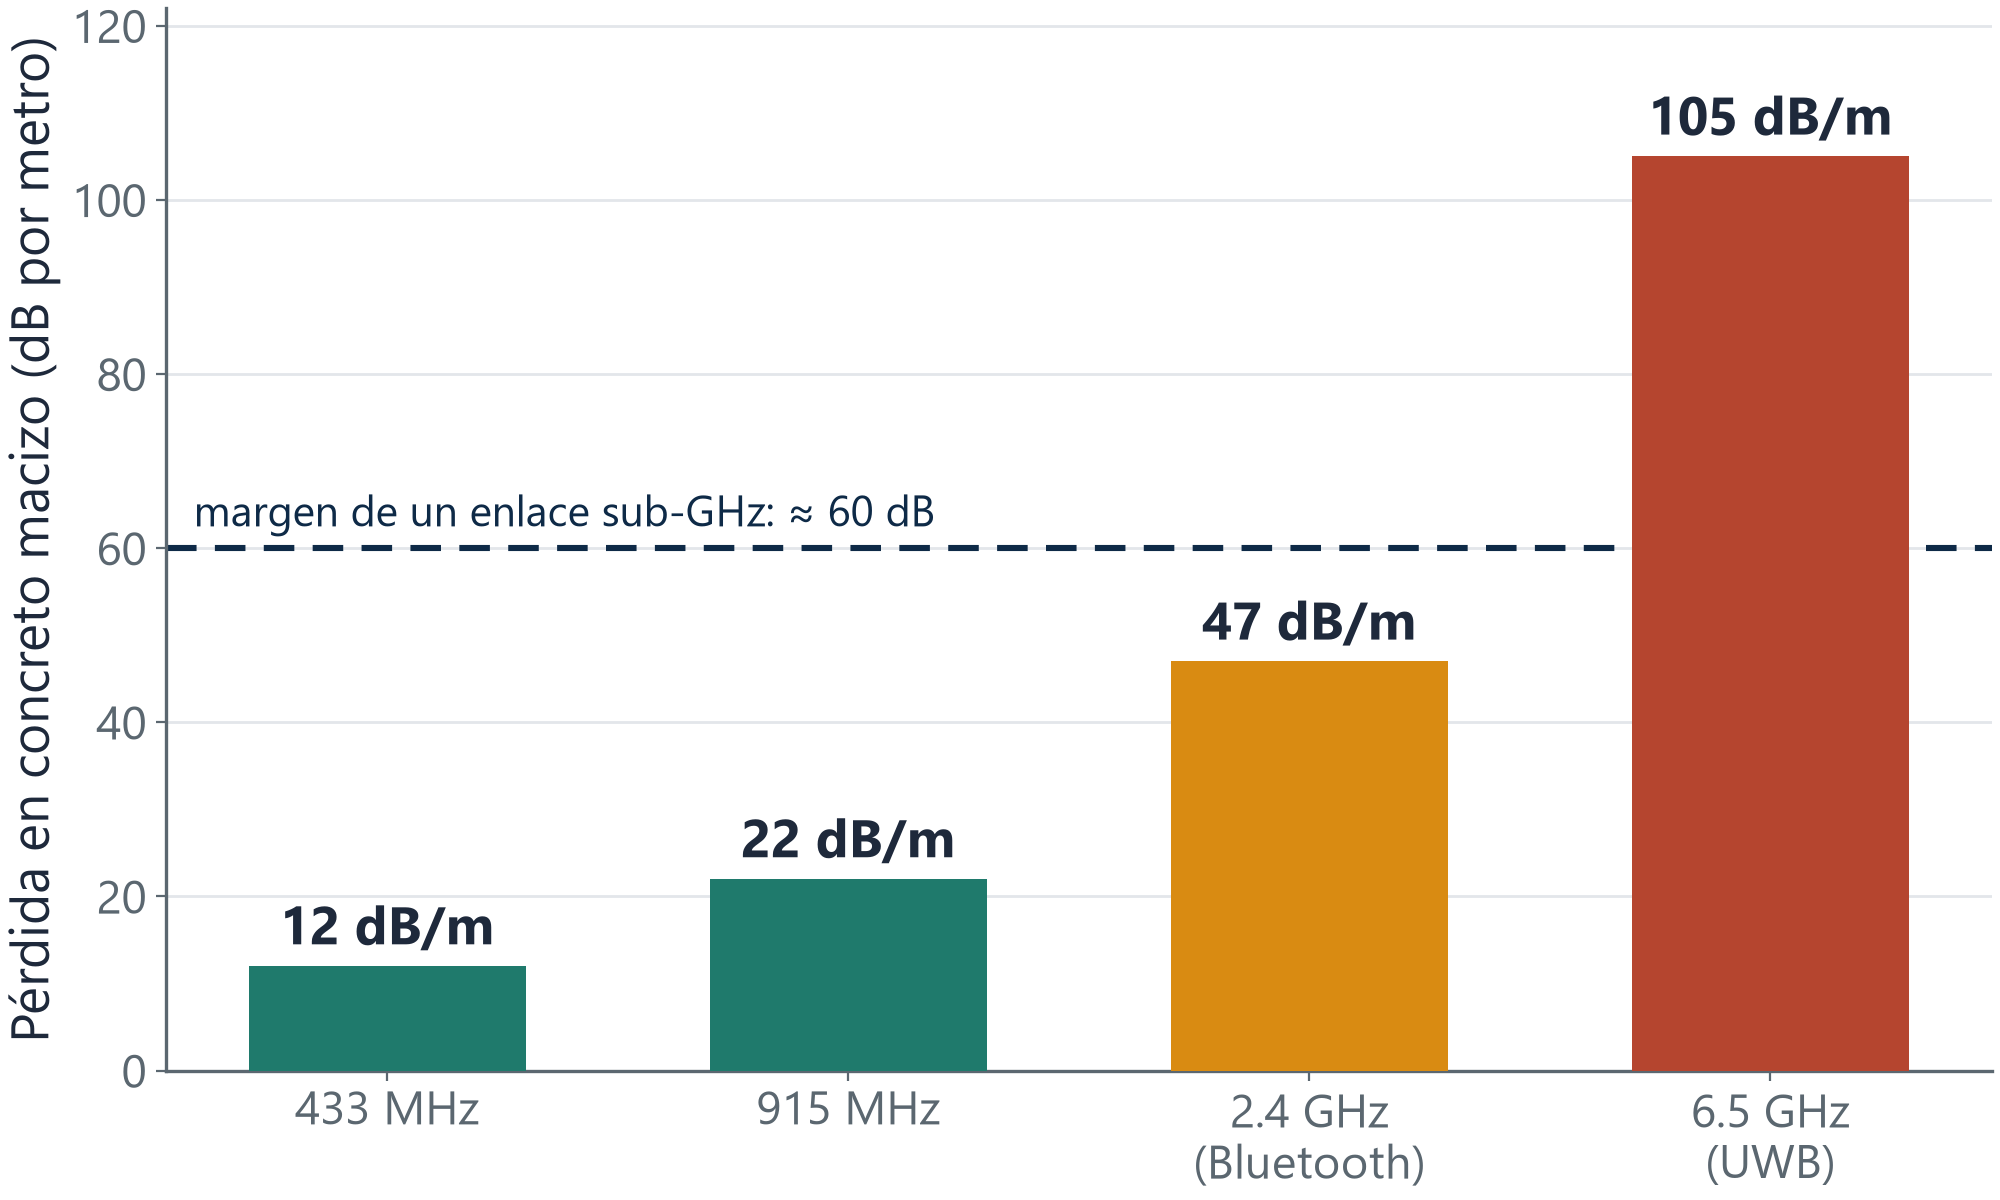
\includegraphics[width=\linewidth]{figs/radio_escombro.png}
\caption{Pérdida de la radio en concreto.}
\label{fig:radio}
\end{subfigure}
\caption{Dos límites prácticos. (a) Contraste térmico disponible y actividad del insecto según la
temperatura~\cite{gracidas2026}. (b) Atenuación calculada con el modelo de la UIT~\cite{itu2040}; las
mediciones de NIST son peores~\cite{stone1997}.}
\end{figure}

\subsection{Localización}

Encontrar a la persona no basta: hay que decirle al rescatista dónde cavar. El método tiene
tres capas, de la más gruesa a la más fina.
\begin{enumerate}
  \item \textbf{Por dónde entró.} Cada mochila tiene un identificador y se libera por un boquete
        conocido. La alerta ya dice en qué zona buscar.
  \item \textbf{Cuánto caminó.} La IMU estima el recorrido contando la actividad de la marcha.
        El error publicado es de 5~\% de la distancia en terreno plano y 10~\% con
        desniveles~\cite{tranngoc2024}: tras 12~m, entre 0.6 y 1.2~m (figura~\ref{fig:localizacion}).
  \item \textbf{El último medio metro.} Al confirmar, la mochila deja de estimular, el insecto se queda
        donde está y emite una baliza de radio y de luz cada 5~s. El tamaño de la mancha da además
        la distancia a la persona: $d\approx\sqrt{A/n}\,/\tan\theta$.
\end{enumerate}
La radio debe ser de menos de 1~GHz. El concreto atenúa unos 22~dB por metro a 915~MHz y 47~dB
a 2.4~GHz~\cite{itu2040}, y el único robot inalámbrico del World Trade Center se perdió a unos
10~m de la entrada~\cite{murphy2004}. Un relevo en el boquete acorta el enlace.

\begin{figure}[H]
\centering
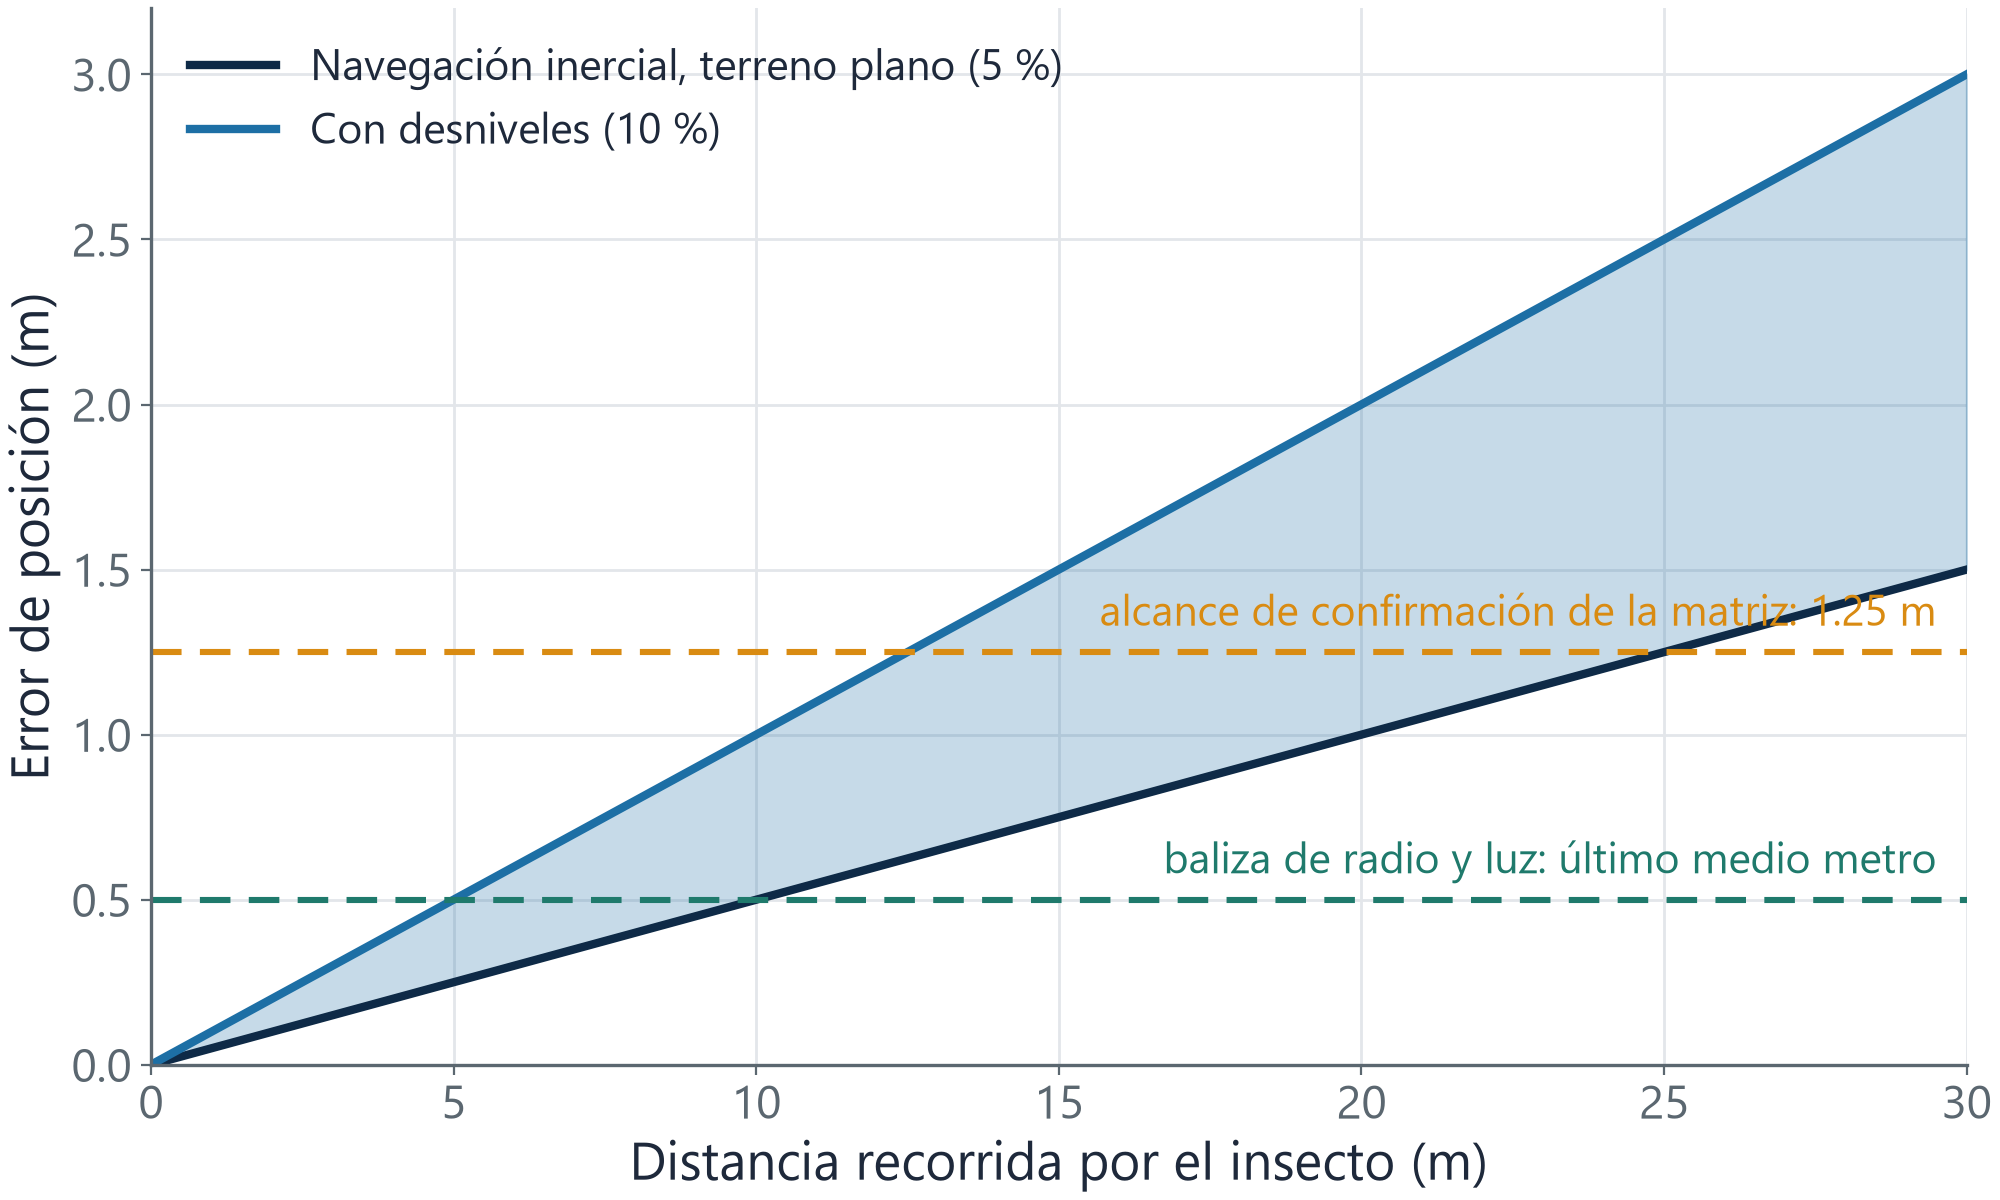
\includegraphics[width=0.62\textwidth]{figs/localizacion.png}
\caption{Error de posición por navegación inercial frente a la distancia recorrida.}
\label{fig:localizacion}
\end{figure}

\subsection{M5. La misión}

La misión se simula con agentes. Cada agente camina con el modelo de M1, obedece estímulos
con el modelo de M2 y detecta con el de M4, dentro de un colapso sintético de $8\times6$~m
hecho de losas y escombro con huecos conectados (figura~\ref{fig:mapa}). Se comparan cuatro
políticas: pasiva (sin estímulos), antipausa, estocástica (antipausa más giros al azar) y guiada
(además se acerca a la mancha de calor). Como referencia analítica, la teoría de búsqueda da
para una búsqueda al azar~\cite{frost2001}
\begin{equation}
P_d=1-e^{-C},\qquad C=\frac{W\,v\,t\,N}{A_h},
\end{equation}
con ancho de barrido $W$, velocidad $v$, tiempo $t$, $N$ insectos y área de huecos $A_h$.

\begin{table}[H]
\centering\footnotesize
\caption{Parámetros principales de la simulación. F: publicado; D: decisión de diseño; S: supuesto que
se explora en el análisis de sensibilidad.}
\label{tab:parametros}
\rowcolors{2}{SoftGray}{white}
\begin{tabularx}{\textwidth}{@{}>{\raggedright\arraybackslash}X >{\raggedright\arraybackslash}p{3.0cm} c >{\raggedright\arraybackslash}p{4.0cm}@{}}
\toprule
\rowcolor{TableHead} \textbf{Parámetro} & \textbf{Valor} & \textbf{Origen} & \textbf{Fuente} \\
\midrule
Velocidad natural & $1.94\pm0.29$~cm/s & F & \cite{dirafzoon2017} \\
Tramo recto, media & 17.6~cm & F & \cite{dirafzoon2017} \\
Probabilidad de pausa por tramo & 0.211 & F & \cite{dirafzoon2017} \\
Duración de la pausa & $36.8\pm24.1$~s & F & \cite{dirafzoon2017} \\
Probabilidad de soltar la pared & 0.005 & F & \cite{dirafzoon2017} \\
Probabilidad de obedecer un estímulo & 0.78 & F & \cite{lin2023} \\
Giro por estímulo & $52\pm23$\textdegree & F & \cite{lin2023,lin2025,ma2023} \\
Marcha tras un estímulo de avance & 5~cm/s durante 4~s & F & \cite{tranngoc2024,erickson2015} \\
Habituación por estímulo, $\alpha$ & 0.01 (0.09 unipolar) & F & \cite{erickson2015,ma2023} \\
Recuperación, $\tau$ & 600~s & F & \cite{sanchez2015} \\
Espera antes de reactivar & 15~s, se duplica hasta $\times8$ & D & --- \\
Tiempo mínimo entre estímulos & 10~s & D & como~\cite{ma2023} \\
Giros al azar & uno cada 51~s en promedio & D & --- \\
Presupuesto de estímulos & 12 acumulados; se vacía en 600~s & D & --- \\
Píxeles para acercar y para confirmar & 2 y 8, cuatro cuadros & D & \cite{tranngoc2024} \\
Área de piel a la vista & 0.03~m$^2$ & S & --- \\
Dobla esquinas pegado a la pared & 0.80 & S & --- \\
Insectos perdidos por hora & 0 & S & --- \\
\bottomrule
\end{tabularx}
\end{table}

\section{Arquitectura embebida}

\subsection{La política que corre a bordo}

La mochila deja que el insecto explore solo y estimula lo mínimo. La política es una máquina
de ocho estados que avanza una vez por cuadro térmico, diez veces por segundo
(figura~\ref{fig:fsm}). Usa tres entradas: cuántos píxeles calientes hay y de qué lado, si el
insecto está quieto según la IMU, y un número al azar.

\begin{figure}[H]
\centering
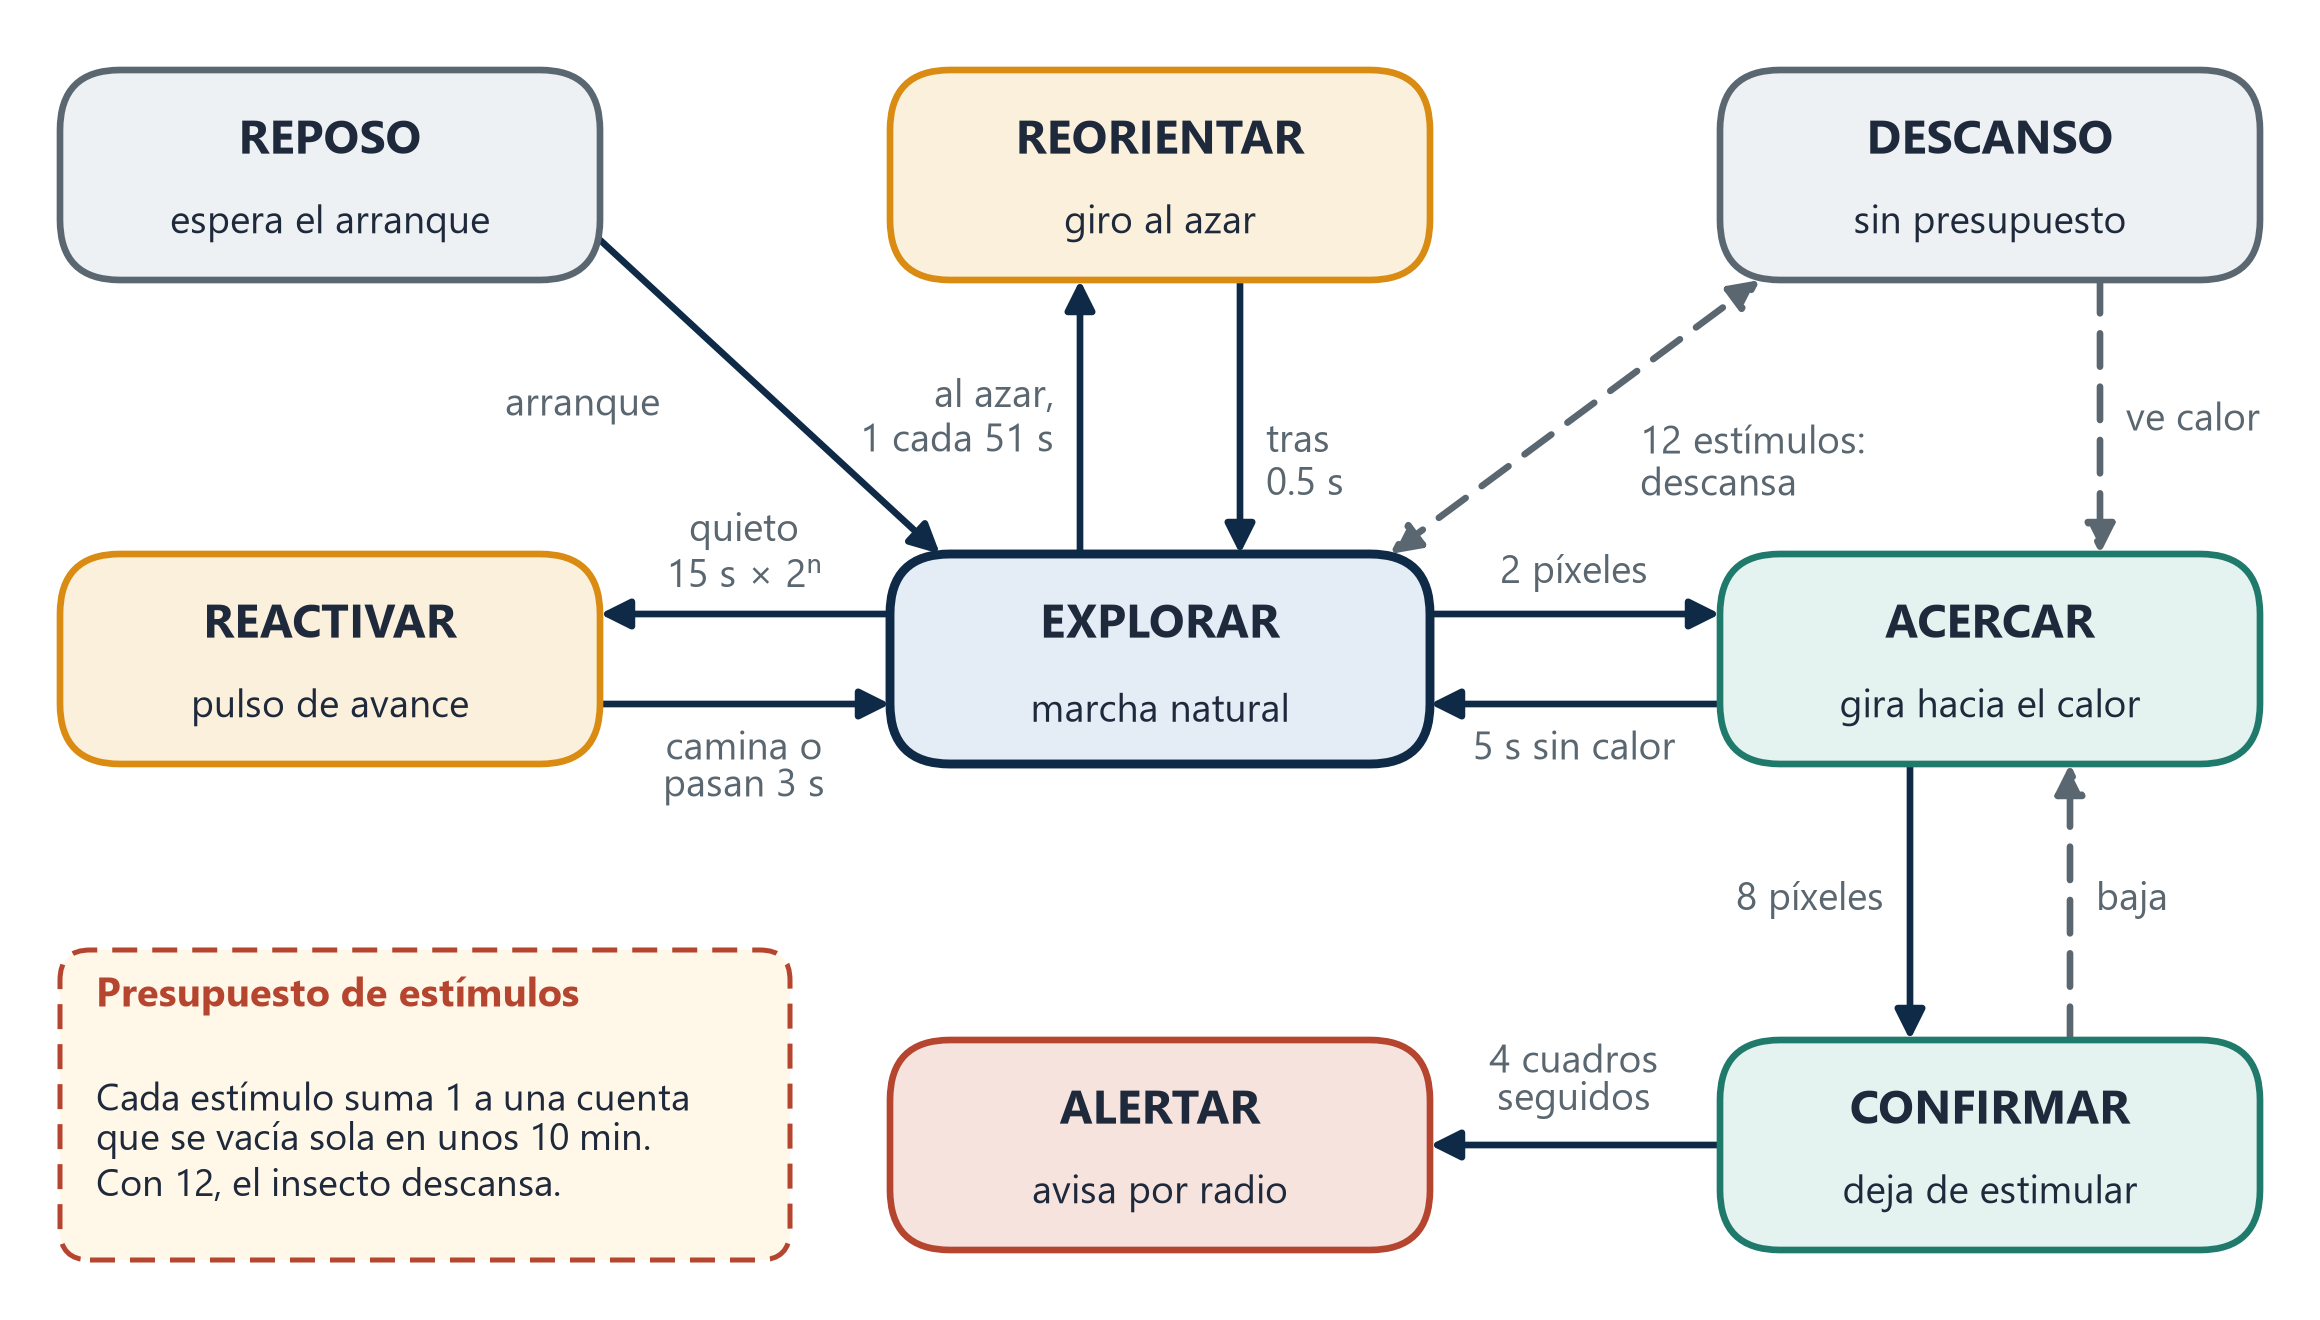
\includegraphics[width=0.86\textwidth]{figs/fsm_politica.png}
\caption{Máquina de estados de la política. Las flechas punteadas no producen estímulo.}
\label{fig:fsm}
\end{figure}

Tres reglas la distinguen de un control remoto:
\begin{itemize}
  \item \textbf{Espera que se duplica.} Si el insecto lleva 15~s quieto recibe un pulso de avance. Si
        en 3~s no arranca, la siguiente espera es de 30~s, luego 60 y 120. Un insecto que no responde
        deja de recibir estímulos inútiles.
  \item \textbf{Giros al azar.} En promedio cada 51~s, un giro a un lado elegido al azar. Es lo que
        despega al insecto de la pared que venía siguiendo~\cite{dirafzoon2017}.
  \item \textbf{Presupuesto de estímulos.} Cada estímulo suma 1 a una cuenta que pierde $1/256$ de su
        valor cada 2.3~s, con lo que se vacía con una constante de unos 590~s, cercana a la recuperación
        del insecto. Con 12 acumulados la mochila deja de estimular. Así acota la habituación y la
        carga sobre el animal sin tener que medir su respuesta.
\end{itemize}

\subsection{El núcleo digital}

\begin{figure}[H]
\centering
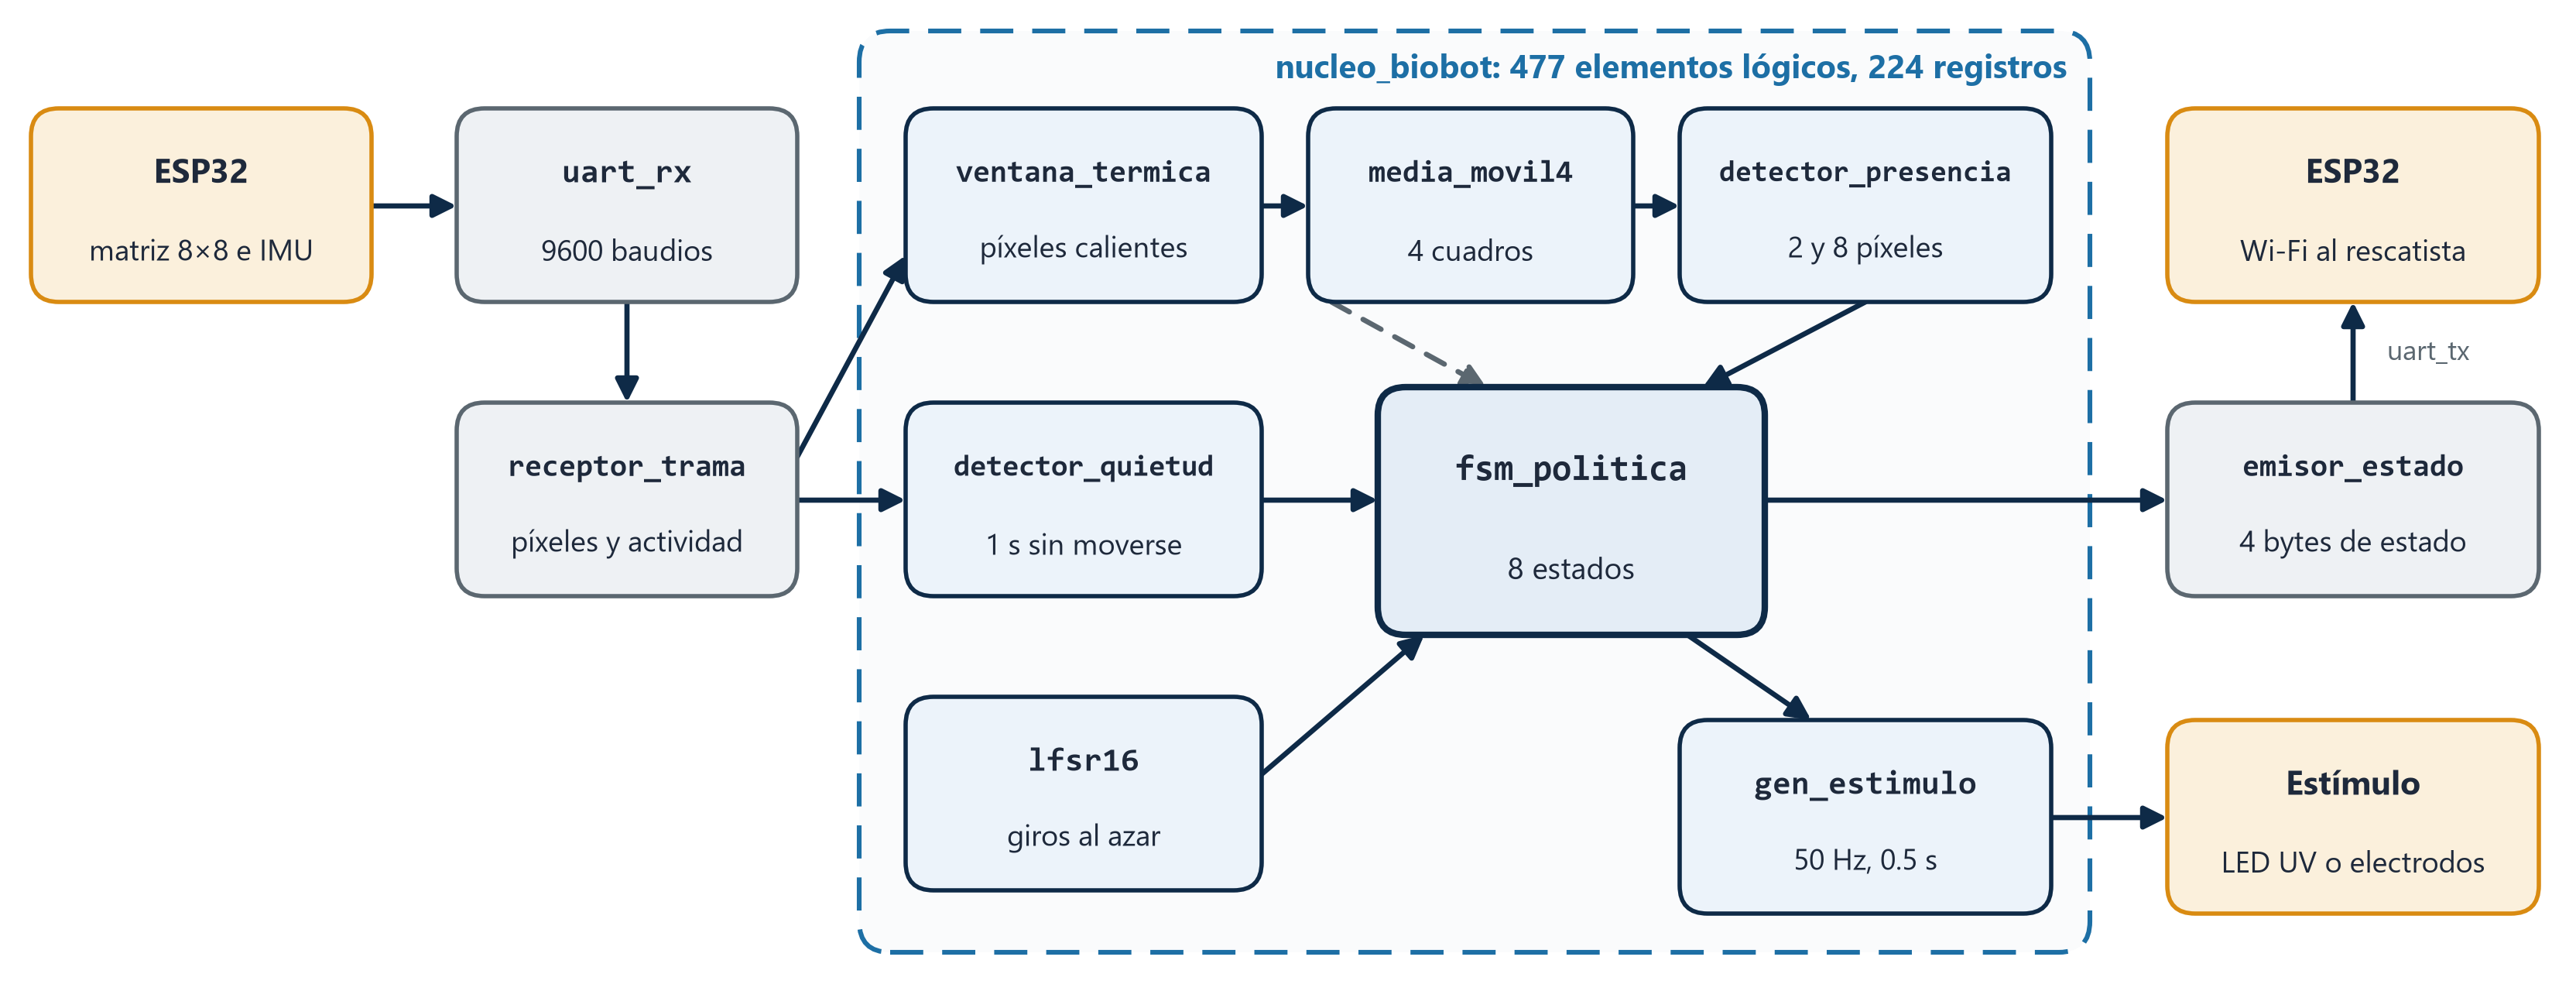
\includegraphics[width=\textwidth]{figs/nucleo_digital.png}
\caption{Módulos Verilog del prototipo. Lo que queda dentro del recuadro punteado es lo que iría en el
chip; lo de fuera es el enlace serie con el ESP32, que en la mochila se sustituye por el lector del
sensor y por la radio.}
\label{fig:nucleo}
\end{figure}

\begin{table}[H]
\centering\footnotesize
\caption{Módulos del núcleo y recursos tras la síntesis en Quartus Prime 24.1 para el
\sig{10M50DAF484C7G}.}
\label{tab:modulos}
\rowcolors{2}{SoftGray}{white}
\begin{tabularx}{\textwidth}{@{}>{\ttfamily\raggedright\arraybackslash}p{3.3cm} >{\raggedright\arraybackslash}X r r@{}}
\toprule
\rowcolor{TableHead} \normalfont\textbf{Módulo} & \textbf{Función} & \textbf{Elem. lógicos} & \textbf{Registros} \\
\midrule
ventana\_termica & Recibe el cuadro píxel por píxel; cuenta los calientes, dice de qué lado están y calcula la media del cuadro & 160 & 61 \\
media\_movil4 & Promedia los últimos cuatro conteos para quitar el vaivén de la marcha & 40 & 28 \\
detector\_presencia & Compara con 2 y con 8 píxeles y exige cuatro cuadros seguidos & 9 & 4 \\
detector\_quietud & Declara quieto al insecto tras 1~s sin actividad en la IMU & 10 & 4 \\
lfsr16 & Números seudoaleatorios para los giros & 16 & 16 \\
fsm\_politica & Los ocho estados, la espera que se duplica y el presupuesto de estímulos & 181 & 64 \\
gen\_estimulo & Tren bifásico de 50~Hz y 0.5~s por el canal pedido & 64 & 47 \\
\midrule
\normalfont\textbf{Núcleo} & & \textbf{477} & \textbf{224} \\
\normalfont Enlace serie y displays & \sig{uart\_rx}, \sig{uart\_tx}, \sig{receptor\_trama}, \sig{emisor\_estado} y decodificadores & 245 & 148 \\
\midrule
\normalfont\textbf{Prototipo completo} & 43 pines, $f_{\max}=72.08$~MHz, holgura de 6.13~ns a 50~MHz & \textbf{722} & \textbf{372} \\
\bottomrule
\end{tabularx}
\end{table}

\subsection{Verificación}

Antes de escribir el Verilog se programó un modelo de referencia en Python que hace las mismas
cuentas con enteros, registro por registro. Ese modelo genera los cuadros de prueba y la
respuesta esperada; los bancos de prueba comparan cuadro por cuadro.

\begin{table}[H]
\centering\footnotesize
\caption{Resultados de simulación con Icarus Verilog 12.}
\label{tab:bancos}
\rowcolors{2}{SoftGray}{white}
\begin{tabularx}{\textwidth}{@{}>{\ttfamily\raggedright\arraybackslash}p{2.8cm} >{\raggedright\arraybackslash}X >{\raggedright\arraybackslash}p{4.4cm}@{}}
\toprule
\rowcolor{TableHead} \normalfont\textbf{Banco} & \textbf{Qué prueba} & \textbf{Resultado} \\
\midrule
tb\_nucleo & 11\,424 cuadros: exploración con pausas, insecto que no responde, acercamiento y detección, ambiente a 30 y 37.5~\textdegree C, objeto a 47.5~\textdegree C y 3\,000 cuadros al azar & 11\,424 de 11\,424 coinciden; se visitan los ocho estados \\
tb\_gen\_estimulo & Periodo, ciclo de trabajo, duración, fases sin traslape y disparo a medio tren & 3 de 3 trenes: 25 periodos de 20.000~ms, 500.0~ms \\
tb\_top & Sistema completo por UART: 500 cuadros hasta la detección confirmada & 500 de 500 respuestas coinciden \\
tb\_demo & Núcleo e insecto de prueba en el mismo chip: persona, sin persona, objeto caliente e insecto que no responde & 4 de 4: solo alerta con persona, en el cuadro 558 \\
tb\_dos\_tarjetas & Dos tarjetas unidas solo por las dos líneas de UART: persona y objeto caliente & 2 de 2: alerta en el cuadro 557; sin alerta con el objeto \\
\bottomrule
\end{tabularx}
\end{table}

El escenario de ambiente tibio confirma el criterio doble de la sección~\ref{sec:deteccion}: con todo el cuadro a
30~\textdegree C no hay píxeles calientes, un objeto a 47.5~\textdegree C no cuenta, y una mancha a
34.5~\textdegree C sí. Con el ambiente a 37.5~\textdegree C la mancha desaparece, que es el límite físico
ya descrito.

\subsection{Camino a un chip propio}

El núcleo usa 224 registros y unos 450 bloques combinacionales. En la biblioteca de alta densidad
de SKY130, un registro ocupa 20.0~$\mu$m$^2$ y una compuerta NAND de dos entradas
3.75~$\mu$m$^2$~\cite{skywater}. Con unos 6~$\mu$m$^2$ por celda combinacional y 50~\% de
utilización, el área estimada es
\begin{equation}
\frac{224\times20.0+450\times6}{0.5}\approx14\,400~\mu\text{m}^2=0.014~\text{mm}^2 ,
\end{equation}
es decir, un módulo de Tiny Tapeout ($160\times100~\mu$m) o dos~\cite{tinytapeout}. Es una
estimación por conteo: el número real saldrá del flujo de SKY130 en la máquina virtual del curso.
Las corridas abiertas cierran el 30 de noviembre de 2026 y entregan chips a mediados de 2027.
Mientras tanto, una iCE40 UltraLite de 1\,248 LUT y 2~mg aloja el núcleo con holgura.

\subsection{Prototipo y demostración}

\begin{figure}[H]
\centering
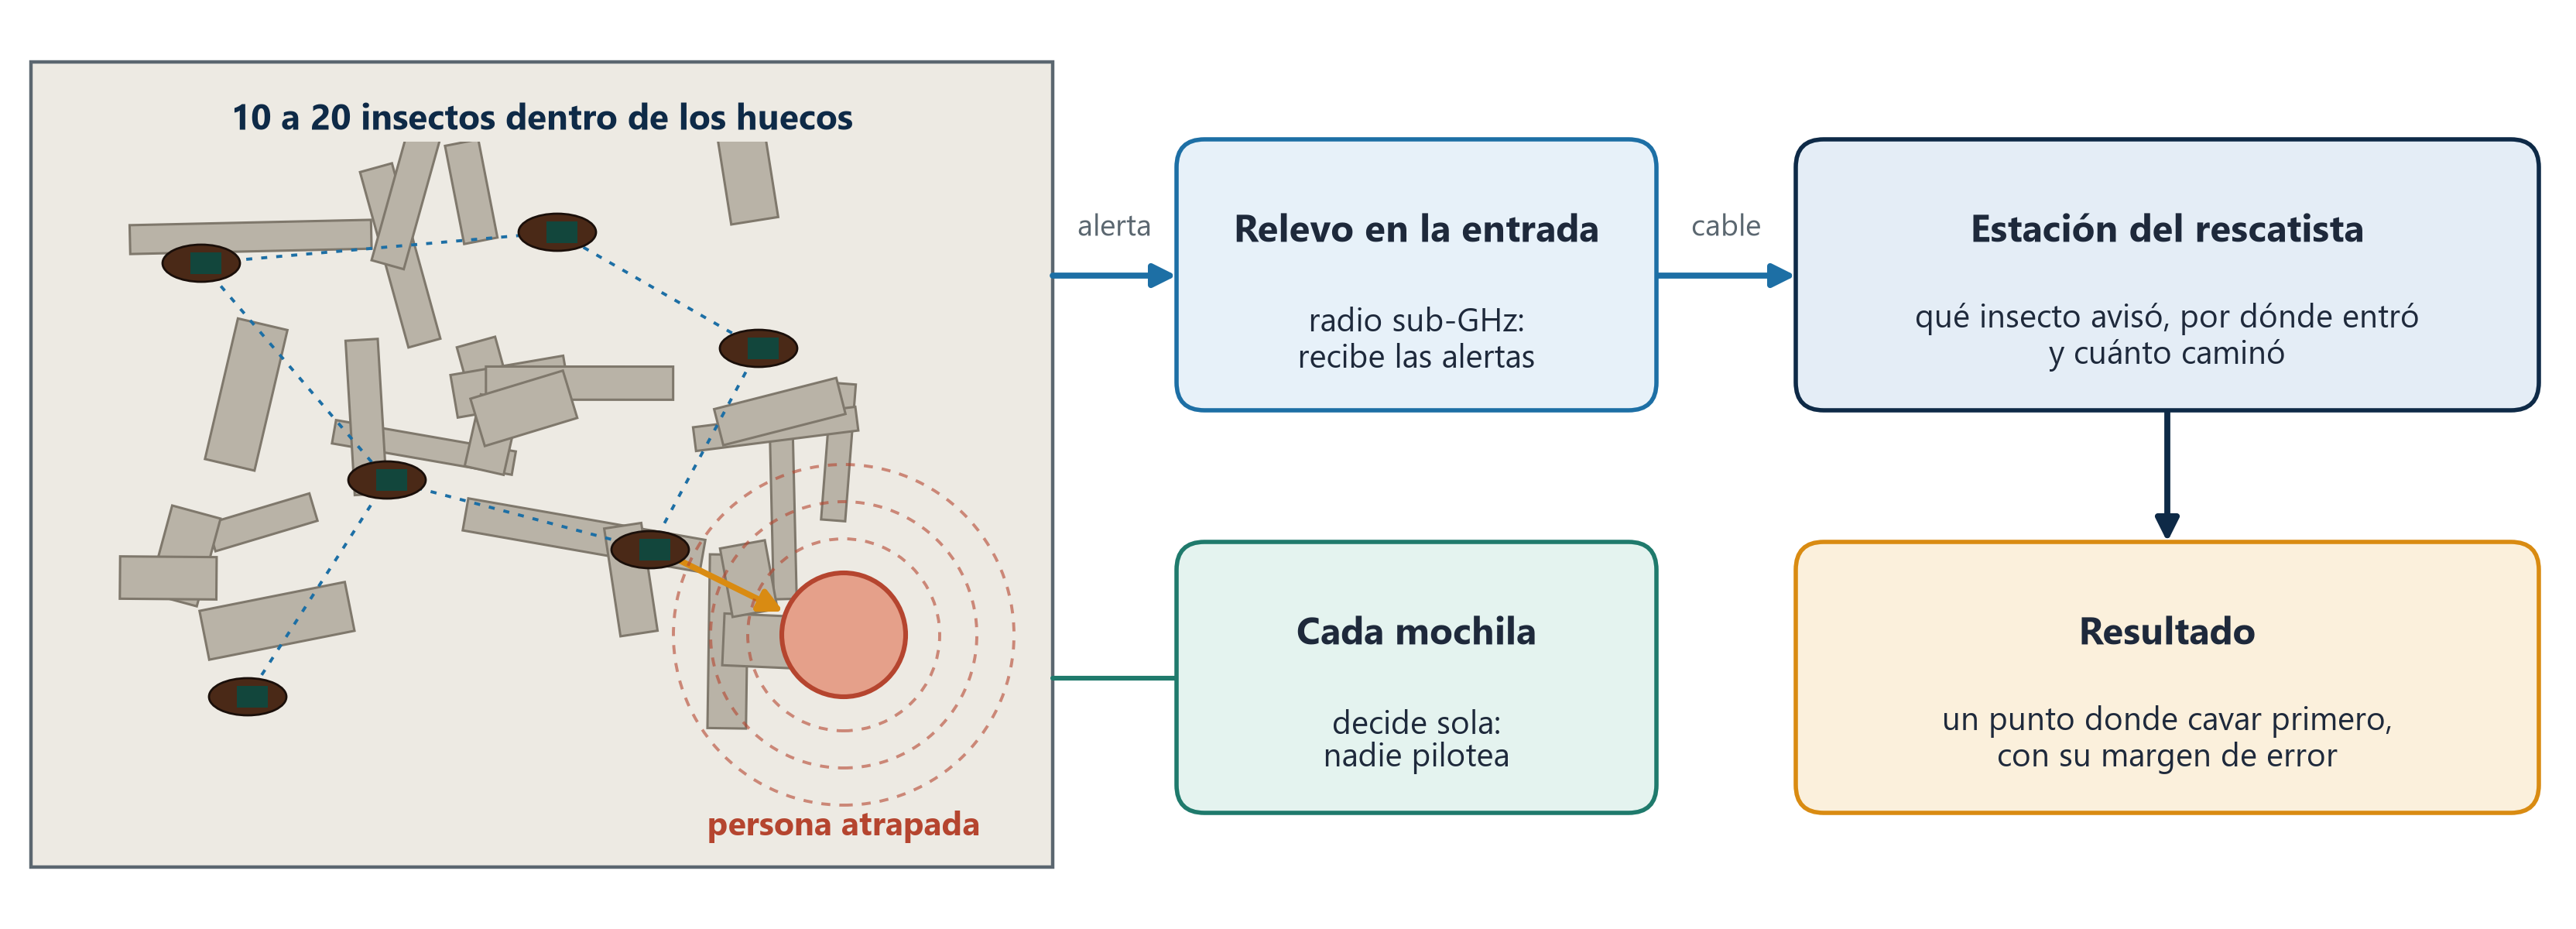
\includegraphics[width=\textwidth]{figs/sistema.png}
\caption{Sistema completo: del enjambre al rescatista.}
\label{fig:sistema}
\end{figure}

En el prototipo, el ESP32 lee la matriz térmica y manda cada cuadro por UART a la DE10-Lite
(66 bytes: encabezado, actividad y 64 píxeles); la tarjeta corre el núcleo y contesta con cuatro
bytes de estado.

\textbf{Prueba en dos tarjetas reales.} Mientras llega el sensor, una segunda DE10-Lite hace de
insecto y de matriz térmica. Calcula los 64 píxeles que vería la mochila según la distancia y el
rumbo, los manda a 9\,600 baudios y mueve a un insecto de prueba según los estímulos que recibe.
Las unen tres cables: dos líneas de UART cruzadas y tierra. El 11 de noviembre de 2026 se corrieron
los cuatro escenarios; los LED y los displays se leyeron por el cable USB con una sonda de Quartus.

\begin{table}[H]
\centering\footnotesize
\caption{Los cuatro escenarios en dos DE10-Lite reales, en tiempo real.}
\label{tab:tarjetas}
\rowcolors{2}{SoftGray}{white}
\begin{tabularx}{\textwidth}{@{}>{\bfseries\raggedright\arraybackslash}p{3.2cm} >{\raggedright\arraybackslash}X >{\raggedright\arraybackslash}p{3.6cm}@{}}
\toprule
\rowcolor{TableHead} Escenario & Lo medido en las tarjetas & Simulación \\
\midrule
Persona a 1.65~m & Acercar a los 26.3~s con 2 píxeles; 8 píxeles a los 54.6~s; alerta a los 55.1~s, cuatro cuadros después; la otra tarjeta recibe la alerta & Alerta a los 55.6~s \\
Objeto a 47.5~\textdegree C & Ningún píxel caliente, ni a 0.2~m; sin alerta en 45~s & Sin alerta \\
Sin persona & Un pulso de avance cuando el insecto se detuvo; sin alerta en 75~s & Sin alerta \\
Insecto que no responde & Reactivar a los 16 y a los 49~s; sin alerta en 75~s & Reactivar a los 16 y a los 49~s \\
\bottomrule
\end{tabularx}
\end{table}

El circuito de la mochila es el mismo que se usará con el ESP32 y el sensor: no se le cambia nada.
El insecto de prueba no es el modelo de marcha de la simulación de misiones; es un banco con
valores redondos que solo sirve para cerrar el lazo. Faltan dos pruebas:
\begin{itemize}
  \item \textbf{Con una persona real.} La matriz apunta a la mesa; al acercar una mano, los LED de
        la tarjeta muestran el paso de explorar a acercar, confirmar y alertar, y el display muestra
        los píxeles calientes.
  \item \textbf{Con un insecto simulado.} La computadora corre la simulación de misión y le manda
        a la tarjeta lo que vería y sentiría la mochila; la tarjeta devuelve los estímulos y la simulación
        mueve al insecto. Es el circuito real dentro del lazo, sin usar animales.
\end{itemize}

\section{Resultados de la simulación}
\label{sec:resultados}

Cada misión libera a los insectos por un boquete de un colapso sintético de $8\times6$~m con
unos \areaLibre~m$^2$ de huecos; la persona está inmóvil, a un recorrido medio de
\distVictima~m de la entrada. Cada configuración se corrió \numCorridas{} veces en
\numMapas{} colapsos distintos: \numMisiones{} misiones de una hora. Con esa muestra, cada
porcentaje tiene un margen de unos $\pm5$ puntos (intervalo de 95~\%).

\subsection{Validación de la marcha}

Antes de comparar políticas se comprobó que el insecto simulado camina como el medido. En una
arena abierta de $1\times1$~m se midieron las mismas magnitudes que
reportan~\cite{dirafzoon2017,tranngoc2024}, primero sin estímulos y luego con comandos al azar.

\begin{table}[H]
\centering\footnotesize
\caption{Marcha simulada frente a la publicada.}
\label{tab:validacion}
\rowcolors{2}{SoftGray}{white}
\begin{tabularx}{0.86\textwidth}{@{}>{\raggedright\arraybackslash}X r r@{}}
\toprule
\rowcolor{TableHead} \textbf{Medida} & \textbf{Publicado} & \textbf{Simulación} \\
\midrule
Fracción del tiempo caminando, sin estímulos & $0.37\pm0.20$ & \valAndaNat \\
Pausa media, sin estímulos (s) & $36.8\pm24.1$ & \valPausaNat \\
Probabilidad de soltar la pared, sin estímulos & 0.005 & \valSalidaNat \\
Fracción del tiempo caminando, con comandos & 0.643 & \valAndaCom \\
Probabilidad de soltar la pared, con comandos & 0.052 & \valSalidaCom \\
Pausa media, con comandos (s) & 5.55 & \valPausaCom \\
\bottomrule
\end{tabularx}
\end{table}

Cinco de las seis medidas coinciden con lo publicado o caen dentro de su dispersión. La que no
coincide es la pausa con comandos: el insecto simulado descansa \valPausaCom~s y el real,
5.6~s. En ese punto el modelo es conservador, porque subestima cuánto acorta las pausas un
estímulo.

\subsection{Cuatro políticas con diez insectos}

Se comparan cuatro políticas. La \textbf{pasiva} solo detecta. La \textbf{antipausa} da un pulso de
avance cuando el insecto lleva 15~s quieto. La \textbf{estocástica} añade giros al azar. La
\textbf{guiada} es la del núcleo: además gira hacia el calor en cuanto la matriz ve dos píxeles.

\begin{figure}[H]
\centering
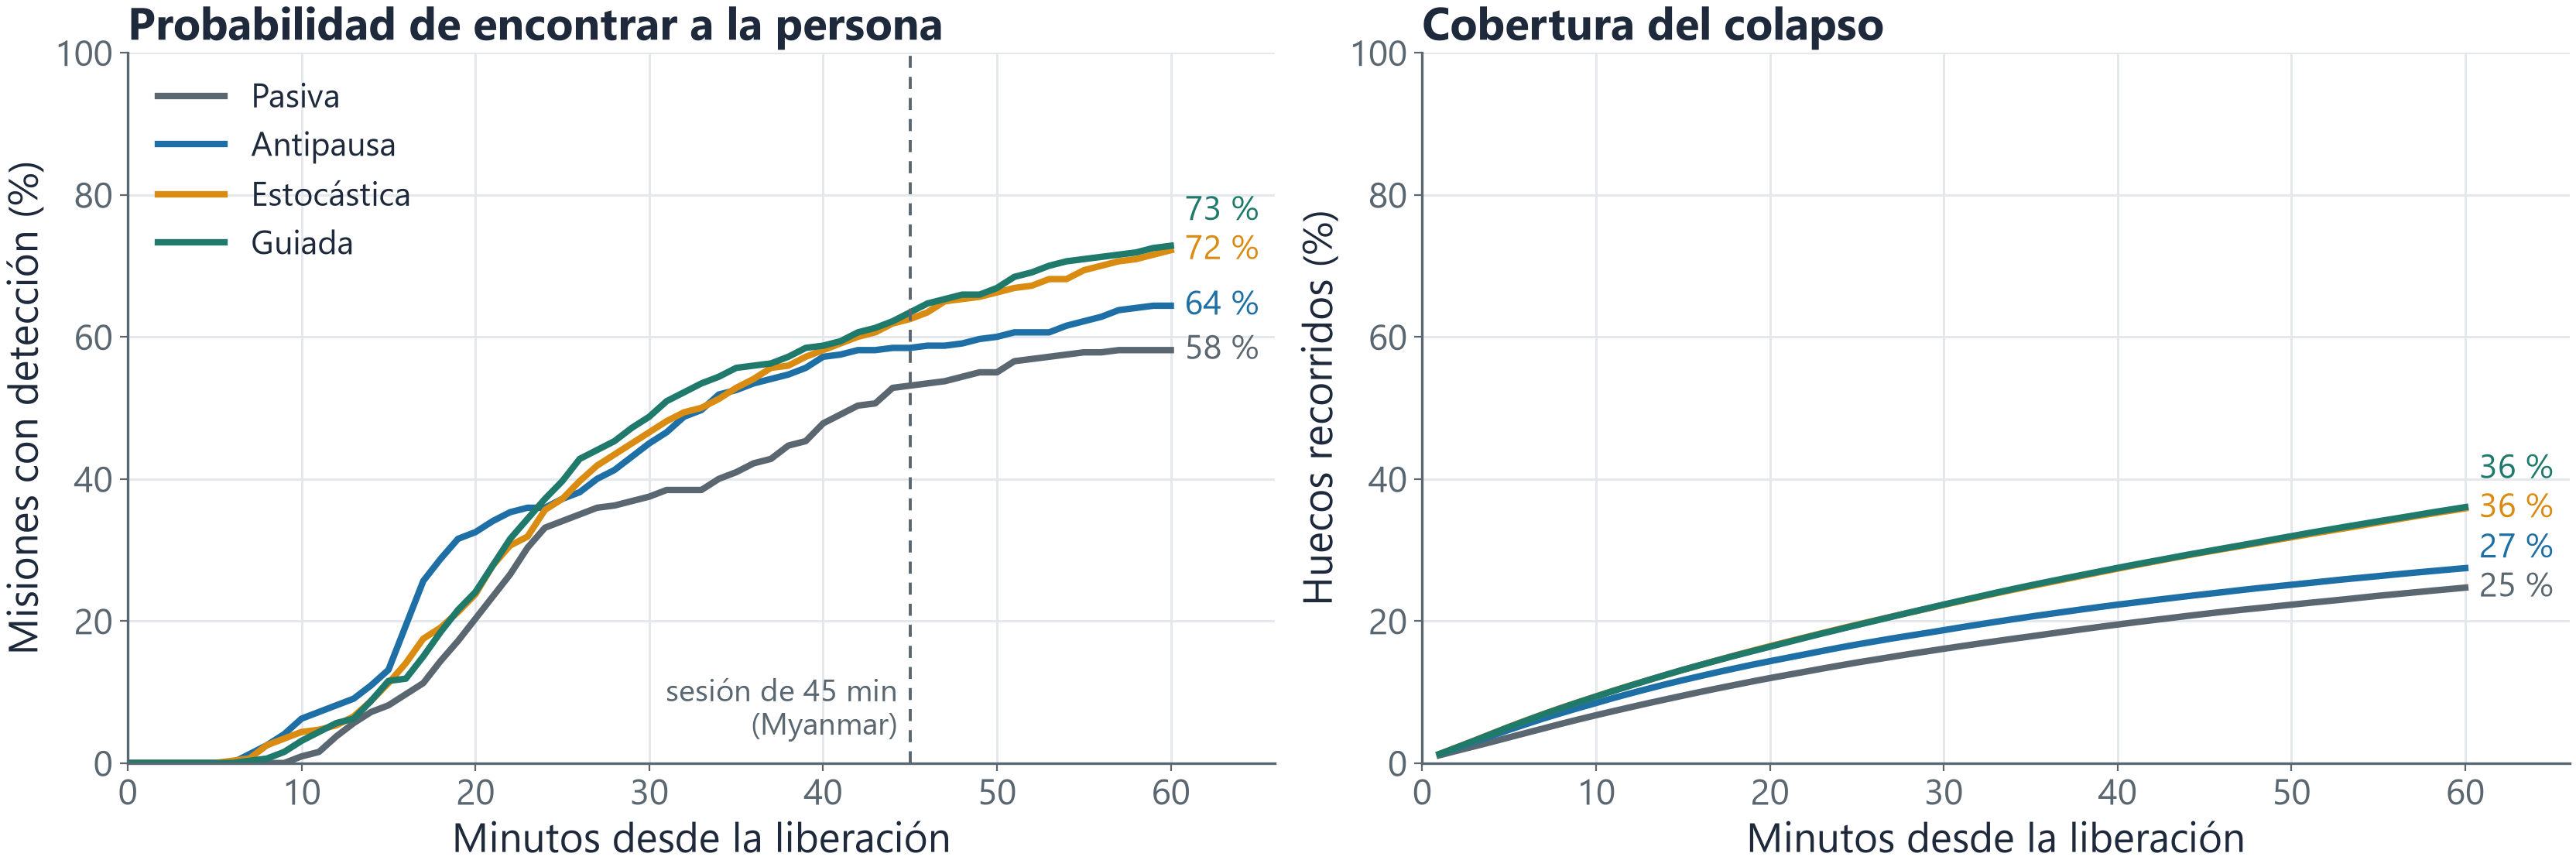
\includegraphics[width=\textwidth]{figs/resultados_politicas.png}
\caption{Diez insectos, \numMisiones{} misiones por política. Izquierda: fracción de misiones en que
algún insecto confirma a la persona. Derecha: fracción de los huecos por los que pasó al menos un insecto.}
\label{fig:politicas}
\end{figure}

\begin{table}[H]
\centering\footnotesize
\caption{Resultados por política con diez insectos. La mediana se calcula entre las misiones que detectan.}
\label{tab:politicas}
\rowcolors{2}{SoftGray}{white}
\begin{tabularx}{\textwidth}{@{}>{\bfseries\raggedright\arraybackslash}X r r r r r r r r@{}}
\toprule
\rowcolor{TableHead} & \multicolumn{4}{c}{\textbf{Detección acumulada (\%)}} & \textbf{Mediana} & \textbf{Cobertura} & \textbf{Estímulos por} & \textbf{Tiempo} \\
\rowcolor{TableHead} \textbf{Política} & 15 min & 30 min & 45 min & 60 min & (min) & (\%) & insecto y hora & caminando (\%) \\
\midrule
\tablaPoliticas
\bottomrule
\end{tabularx}
\end{table}

Sin estímulos, diez insectos encuentran a la persona en \pPasivaSesenta~\% de las misiones de
una hora. Reactivar al insecto cuando se queda quieto sube la cifra a \pAntipausaSesenta~\%;
añadir giros al azar, a \pEstocasticaSesenta~\%; y girar hacia el calor, a \pGuiadaSesenta~\%.
Tres lecturas:
\begin{itemize}
  \item \textbf{La ganancia viene de mantener al insecto en movimiento y despegarlo de las paredes.}
        Girar hacia el calor casi no añade, porque solo actúa dentro del alcance de la matriz.
  \item \textbf{En el primer cuarto de hora las políticas no se distinguen.} La diferencia aparece
        después de la media hora, cuando el insecto sin estímulos acumula pausas.
  \item \textbf{El costo es bajo:} unos \estGuiada{} estímulos por insecto y por hora, uno por minuto,
        siempre por debajo del presupuesto de doce acumulados.
\end{itemize}

\begin{figure}[H]
\centering
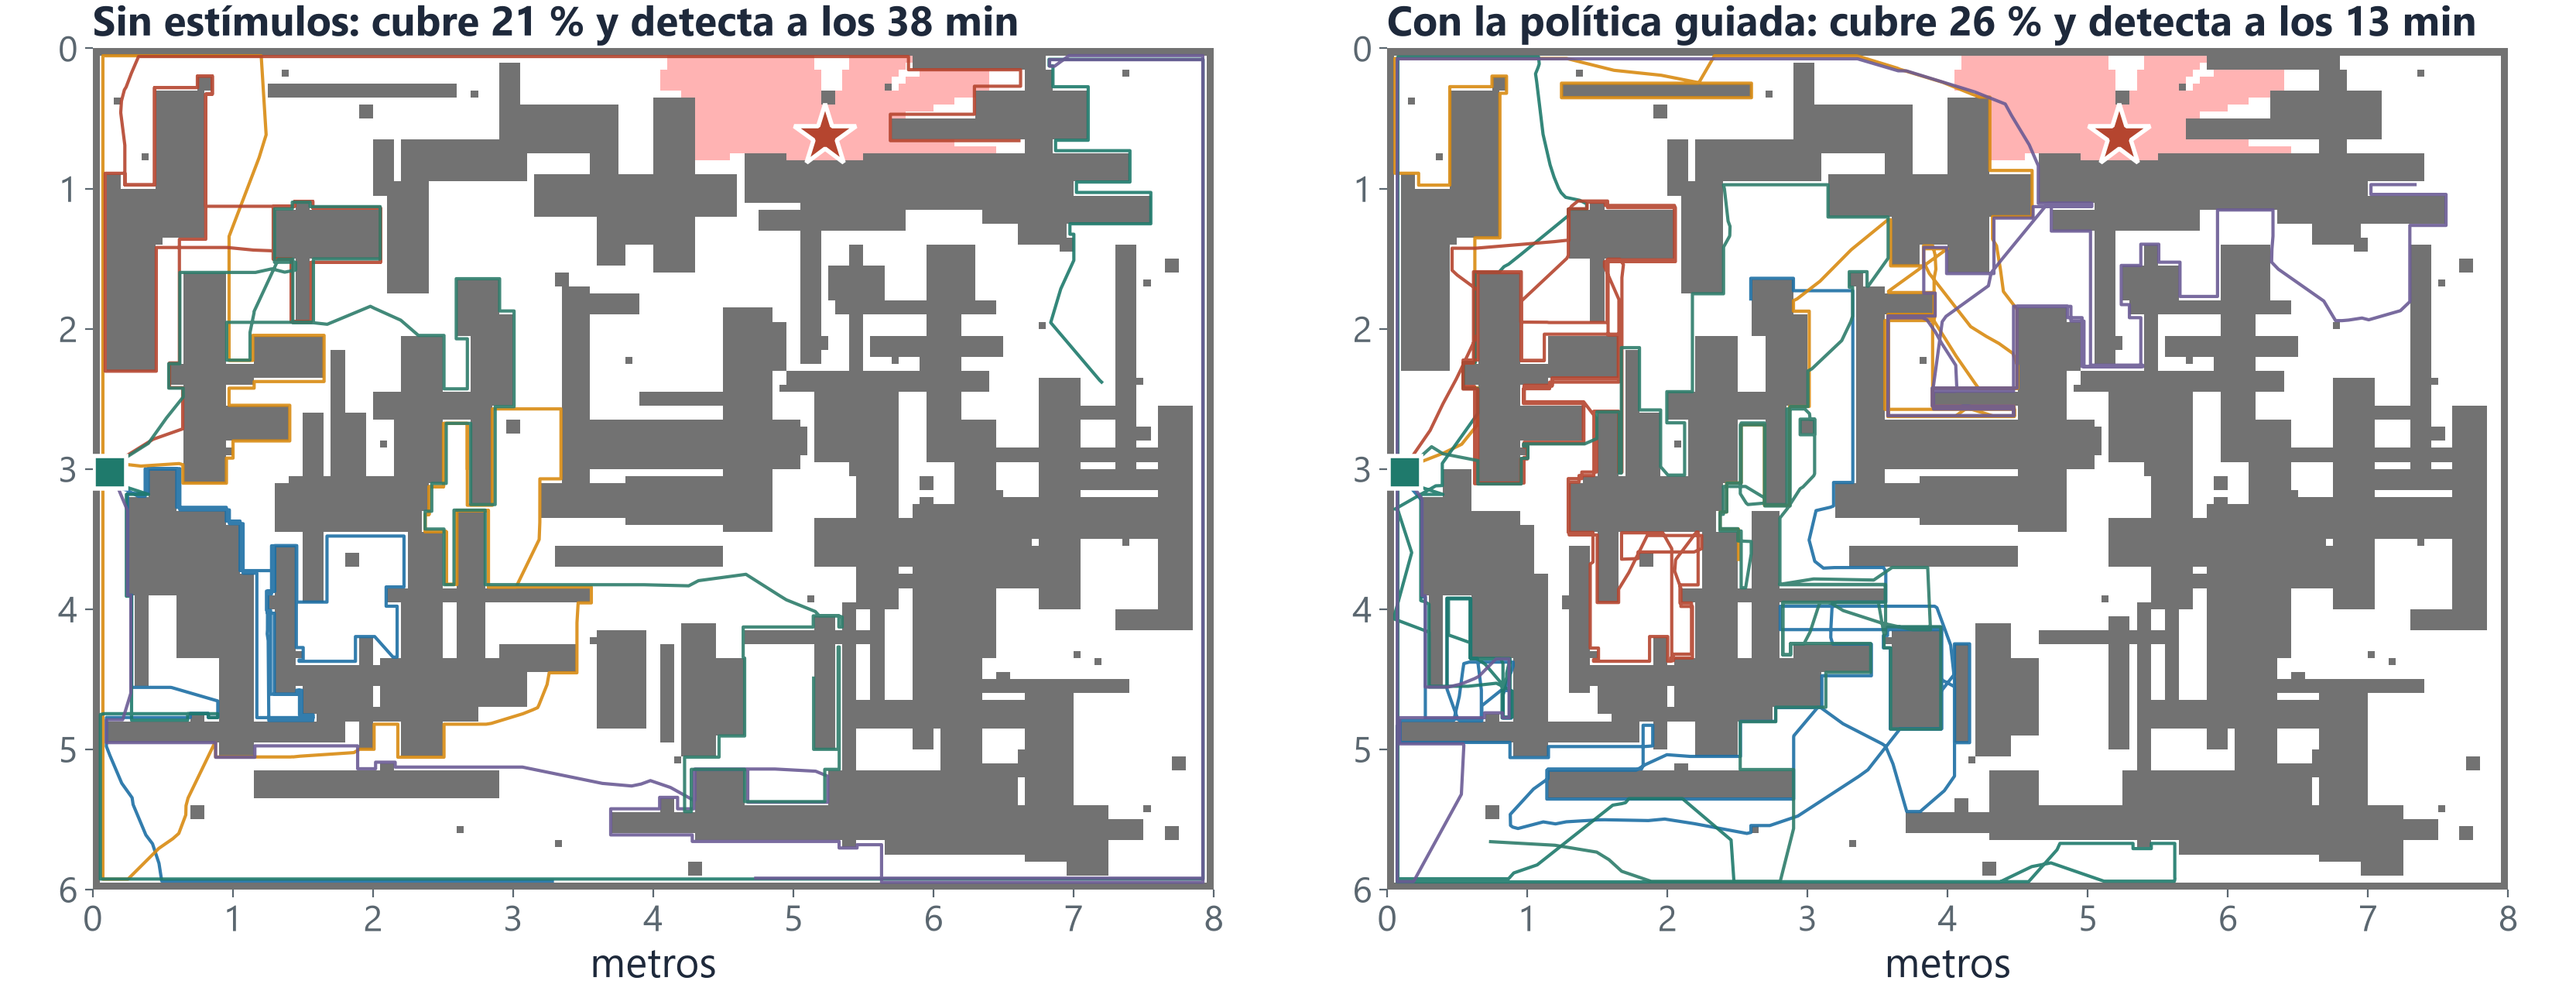
\includegraphics[width=\textwidth]{figs/mapa_trayectorias.png}
\caption{Una misión de ejemplo: seis insectos durante 45~min en el mismo colapso. Cuadro verde: entrada;
estrella: persona; zona sombreada: desde donde la matriz confirma. Una sola corrida no prueba nada; la
comparación válida es la de la figura~\ref{fig:politicas}.}
\label{fig:mapa}
\end{figure}

\subsection{El colapso pesa más que la política}

\begin{figure}[H]
\centering
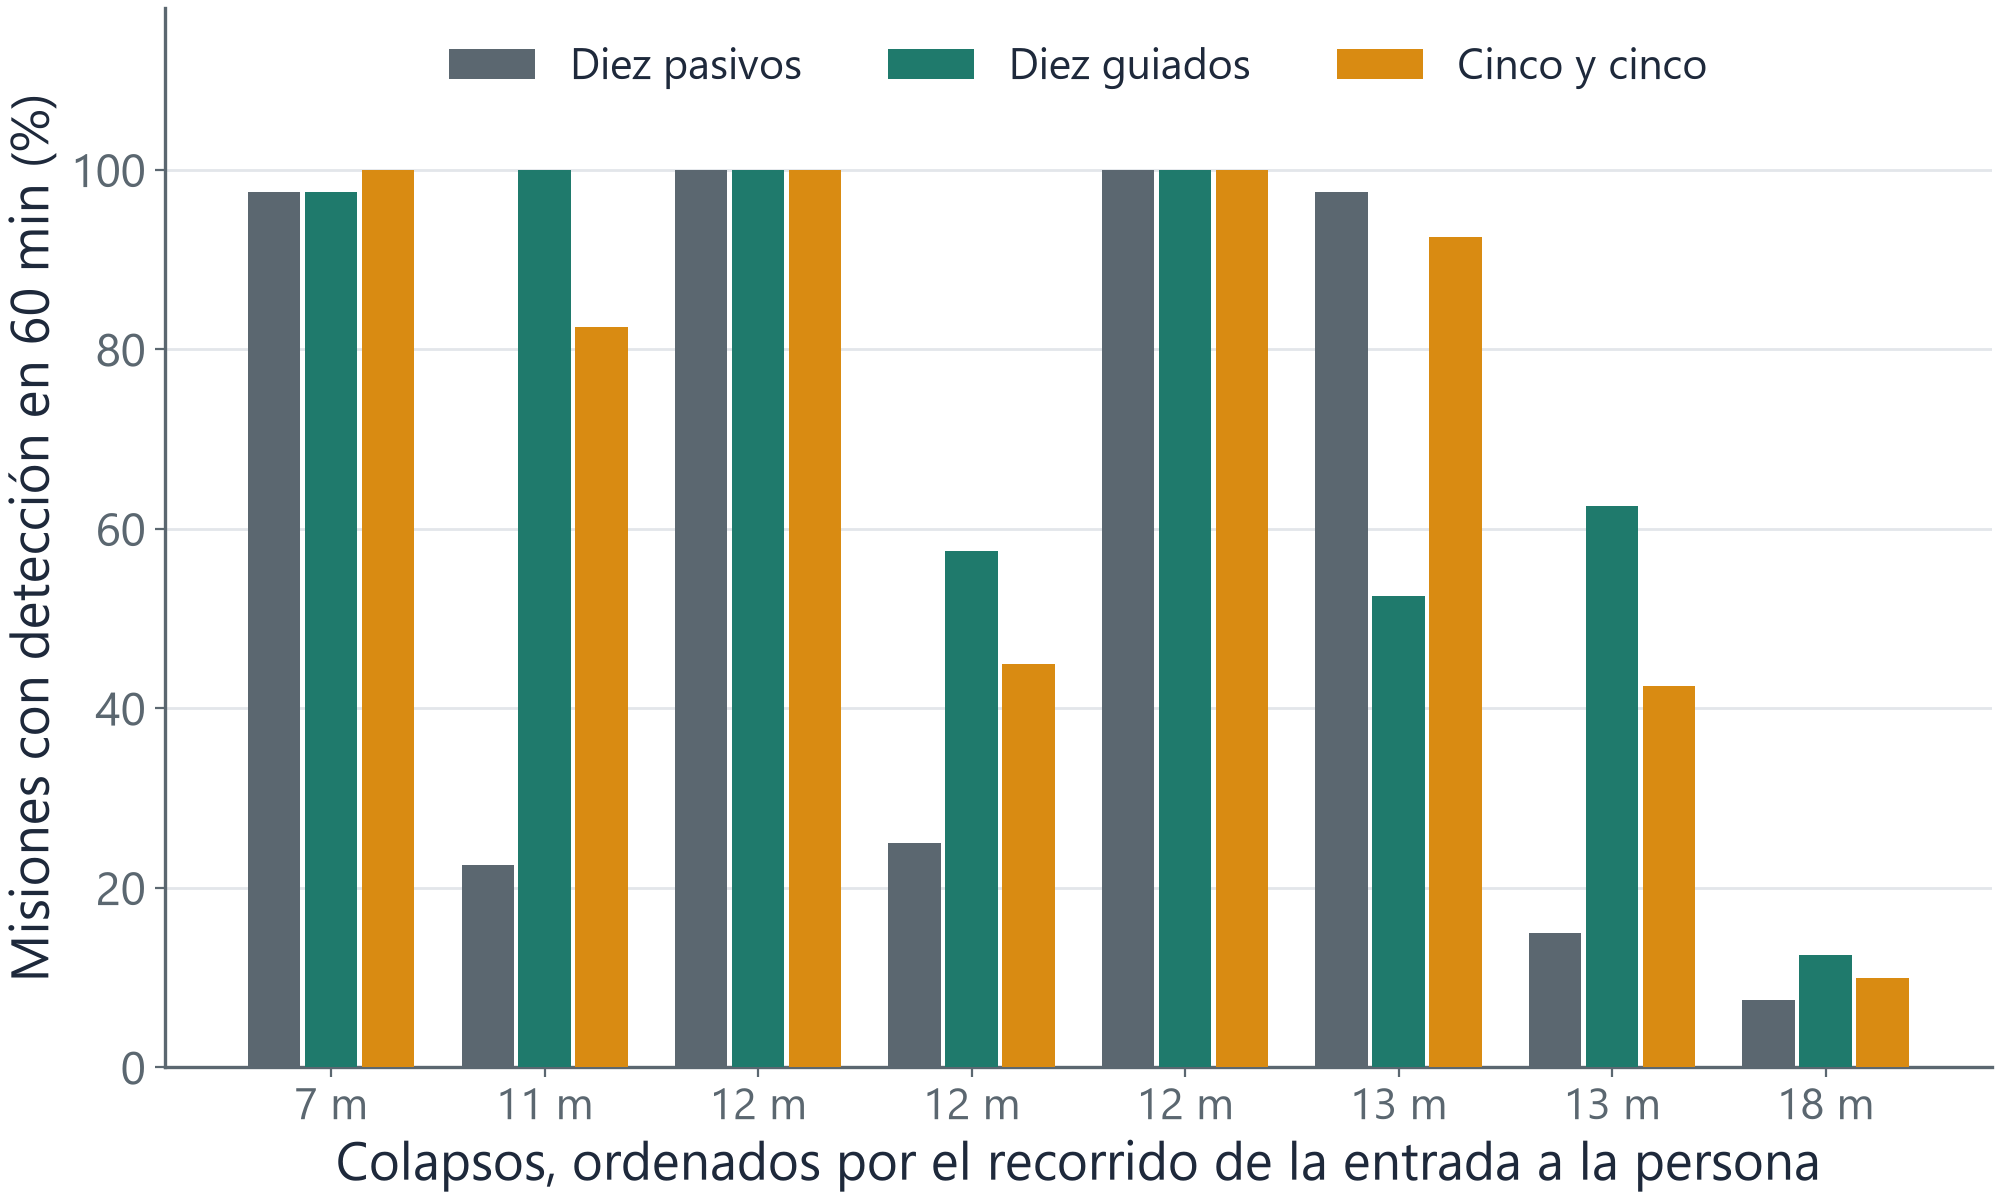
\includegraphics[width=0.7\textwidth]{figs/por_mapa.png}
\caption{Detección a 60~min en cada uno de los ocho colapsos, con diez insectos pasivos, diez guiados y
cinco de cada uno. Cuarenta misiones por barra.}
\label{fig:pormapa}
\end{figure}

El promedio esconde una dispersión grande. Según el colapso, la detección en una hora va de
\mapaMinPasiva{} a \mapaMaxPasiva~\% sin estímulos y de \mapaMinGuiada{} a \mapaMaxGuiada~\%
con la política guiada (figura~\ref{fig:pormapa}). La guiada gana por más de cinco puntos en
\mapasGanaGuiada{} de los \numMapas{} colapsos, empata en \mapasEmpate{} y pierde en
\mapasPierdeGuiada.

En los empates las dos políticas dan lo mismo porque la persona se encuentra de cualquier modo
o porque queda demasiado lejos para ambas. Donde la guiada gana, cambia el resultado por
completo: en el caso más claro, de \mapaMejorPasiva{} a \mapaMejorGuiada~\%. Y donde pierde,
pierde mucho: de \mapaPeorPasiva{} a \mapaPeorGuiada~\%. En ese colapso seguir la pared lleva
directo a la persona, y los giros al azar sacan al insecto de ese camino. El promedio de la
sección anterior, por lo tanto, no describe a ningún colapso en particular: en cada uno el
resultado es casi todo o casi nada, y lo decide la geometría.

\textbf{Un enjambre mixto cubre los dos casos.} Como desde afuera no se sabe qué tipo de colapso
se tiene, se probó liberar cinco insectos sin estímulos y cinco guiados. El promedio no cambia:
\mixtoSesenta~\% en una hora, frente a \pGuiadaSesenta~\% con los diez guiados. Pero desaparece
el caso malo: donde la política guiada caía a \mapaPeorGuiada~\%, el enjambre mixto llega a
\mixtoPeor~\%. A cambio cede parte de la ganancia donde guiar ayuda: \mixtoMejor~\% en lugar de
\mapaMejorGuiada~\% en el mejor caso. Es la configuración que se recomienda mientras no haya
forma de reconocer el colapso antes de entrar. En el núcleo pide un modo de solo detección, que
es un cambio pequeño y queda pendiente.

\subsection{Tamaño del enjambre}

\begin{figure}[H]
\centering
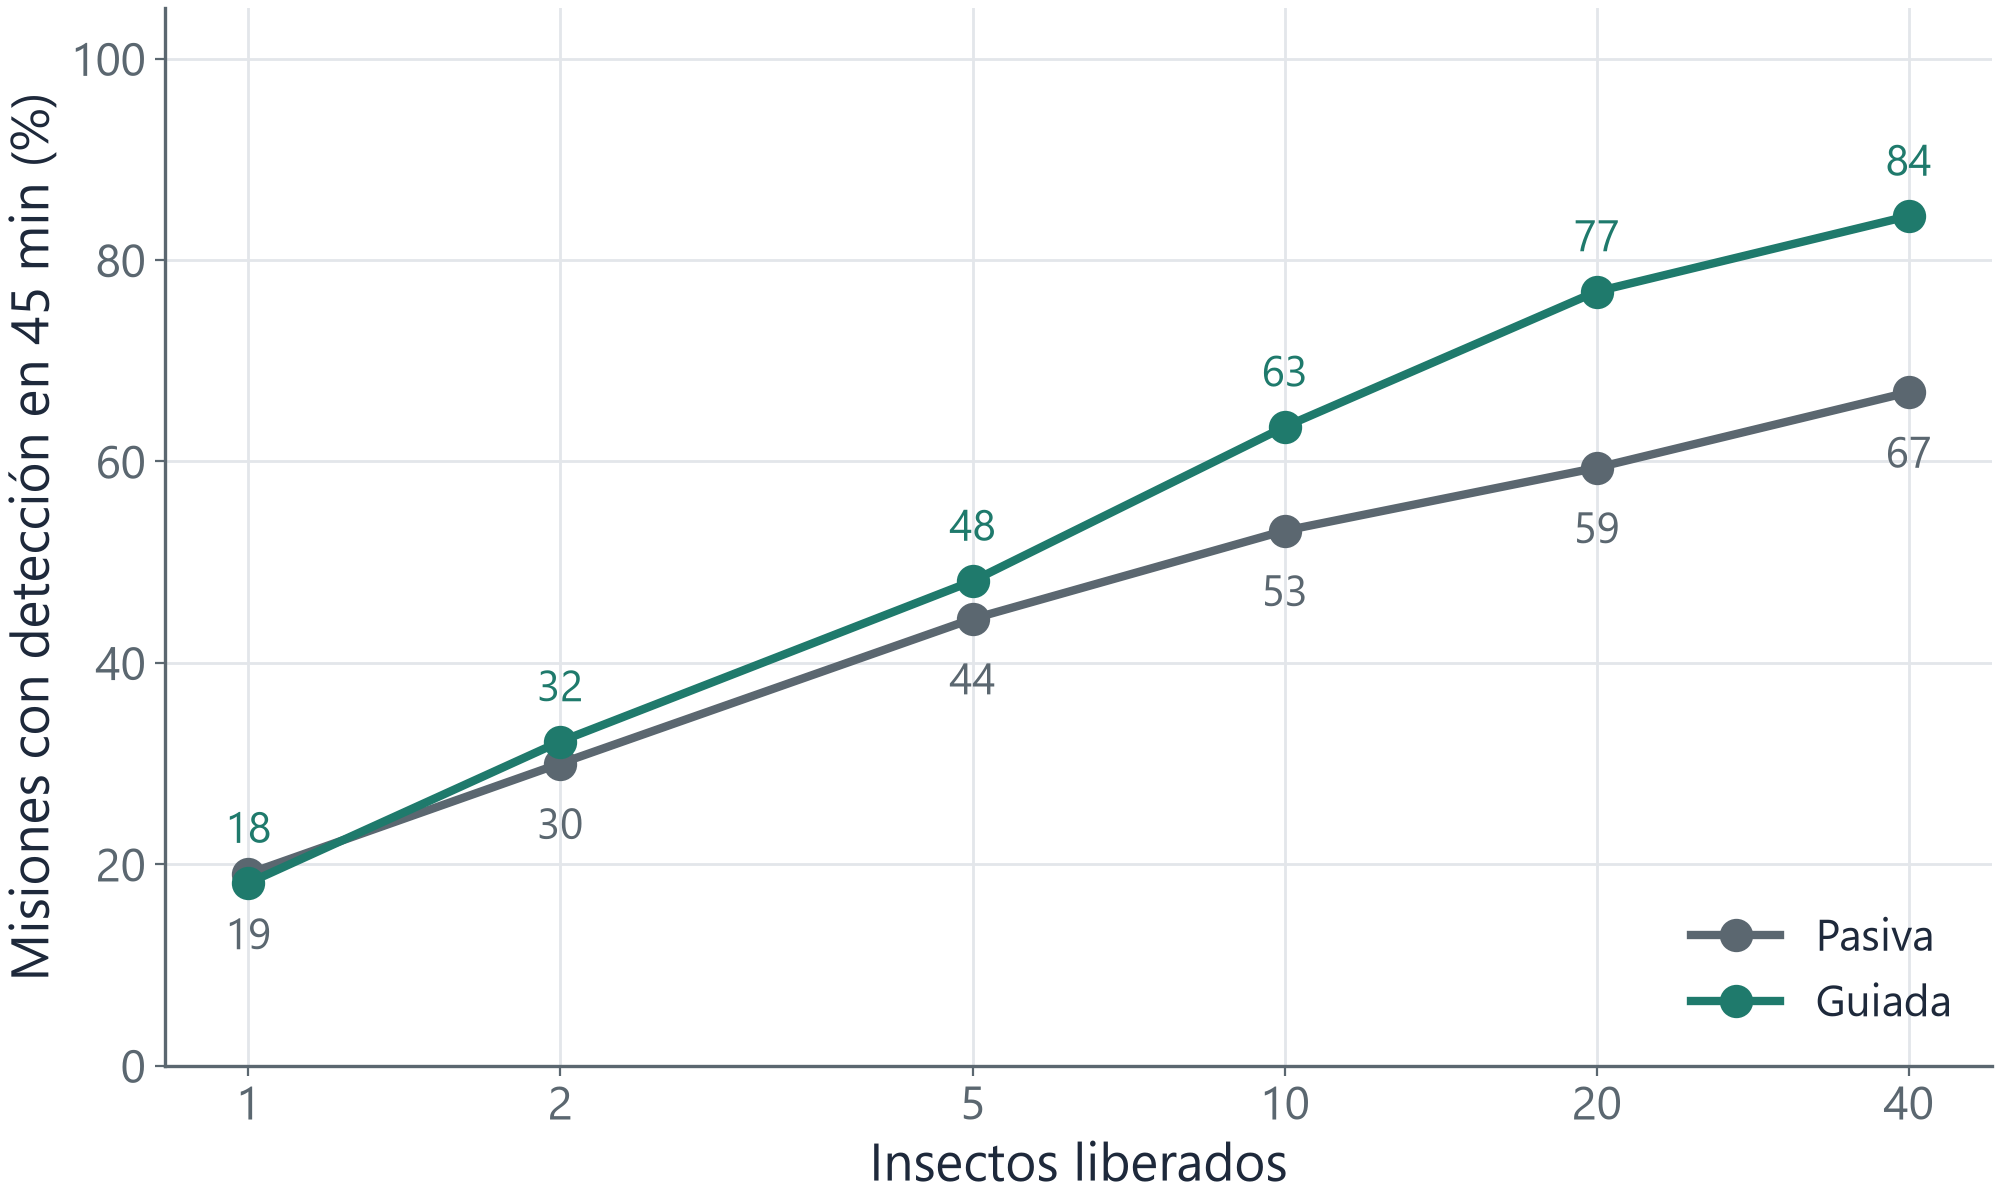
\includegraphics[width=0.62\textwidth]{figs/enjambre.png}
\caption{Detección a 45~min según el número de insectos liberados.}
\label{fig:enjambre}
\end{figure}

\begin{table}[H]
\centering\footnotesize
\caption{Detección acumulada (\%) según el número de insectos liberados.}
\label{tab:enjambre}
\rowcolors{2}{SoftGray}{white}
\begin{tabularx}{0.8\textwidth}{@{}>{\bfseries\raggedright\arraybackslash}X r r r r r r@{}}
\toprule
\rowcolor{TableHead} & \multicolumn{3}{c}{\textbf{Pasiva}} & \multicolumn{3}{c}{\textbf{Guiada}} \\
\rowcolor{TableHead} \textbf{Insectos} & 30 min & 45 min & 60 min & 30 min & 45 min & 60 min \\
\midrule
\tablaEnjambre
\bottomrule
\end{tabularx}
\end{table}

Un insecto solo casi nunca basta: guiado o no, encuentra a la persona en cerca de una de cada
cuatro misiones de una hora (\enjHoraPasivaUno{} y \enjHoraGuiadaUno~\%). La guía empieza a
notarse con cinco insectos y pesa más cuanto mayor es el enjambre: con veinte, la detección en
una hora pasa de \enjHoraPasivaVeinte{} a \enjHoraGuiadaVeinte~\%. Diez insectos guiados
(\enjHoraGuiadaDiez~\%) rinden como entre veinte y cuarenta sin guiar (\enjHoraPasivaVeinte{} y
\enjHoraPasivaCuarenta~\%). Dicho de otro modo, la política equivale a duplicar o triplicar el
enjambre sin criar ni equipar más animales.

\subsection{Sensor y habituación}

\begin{figure}[H]
\centering
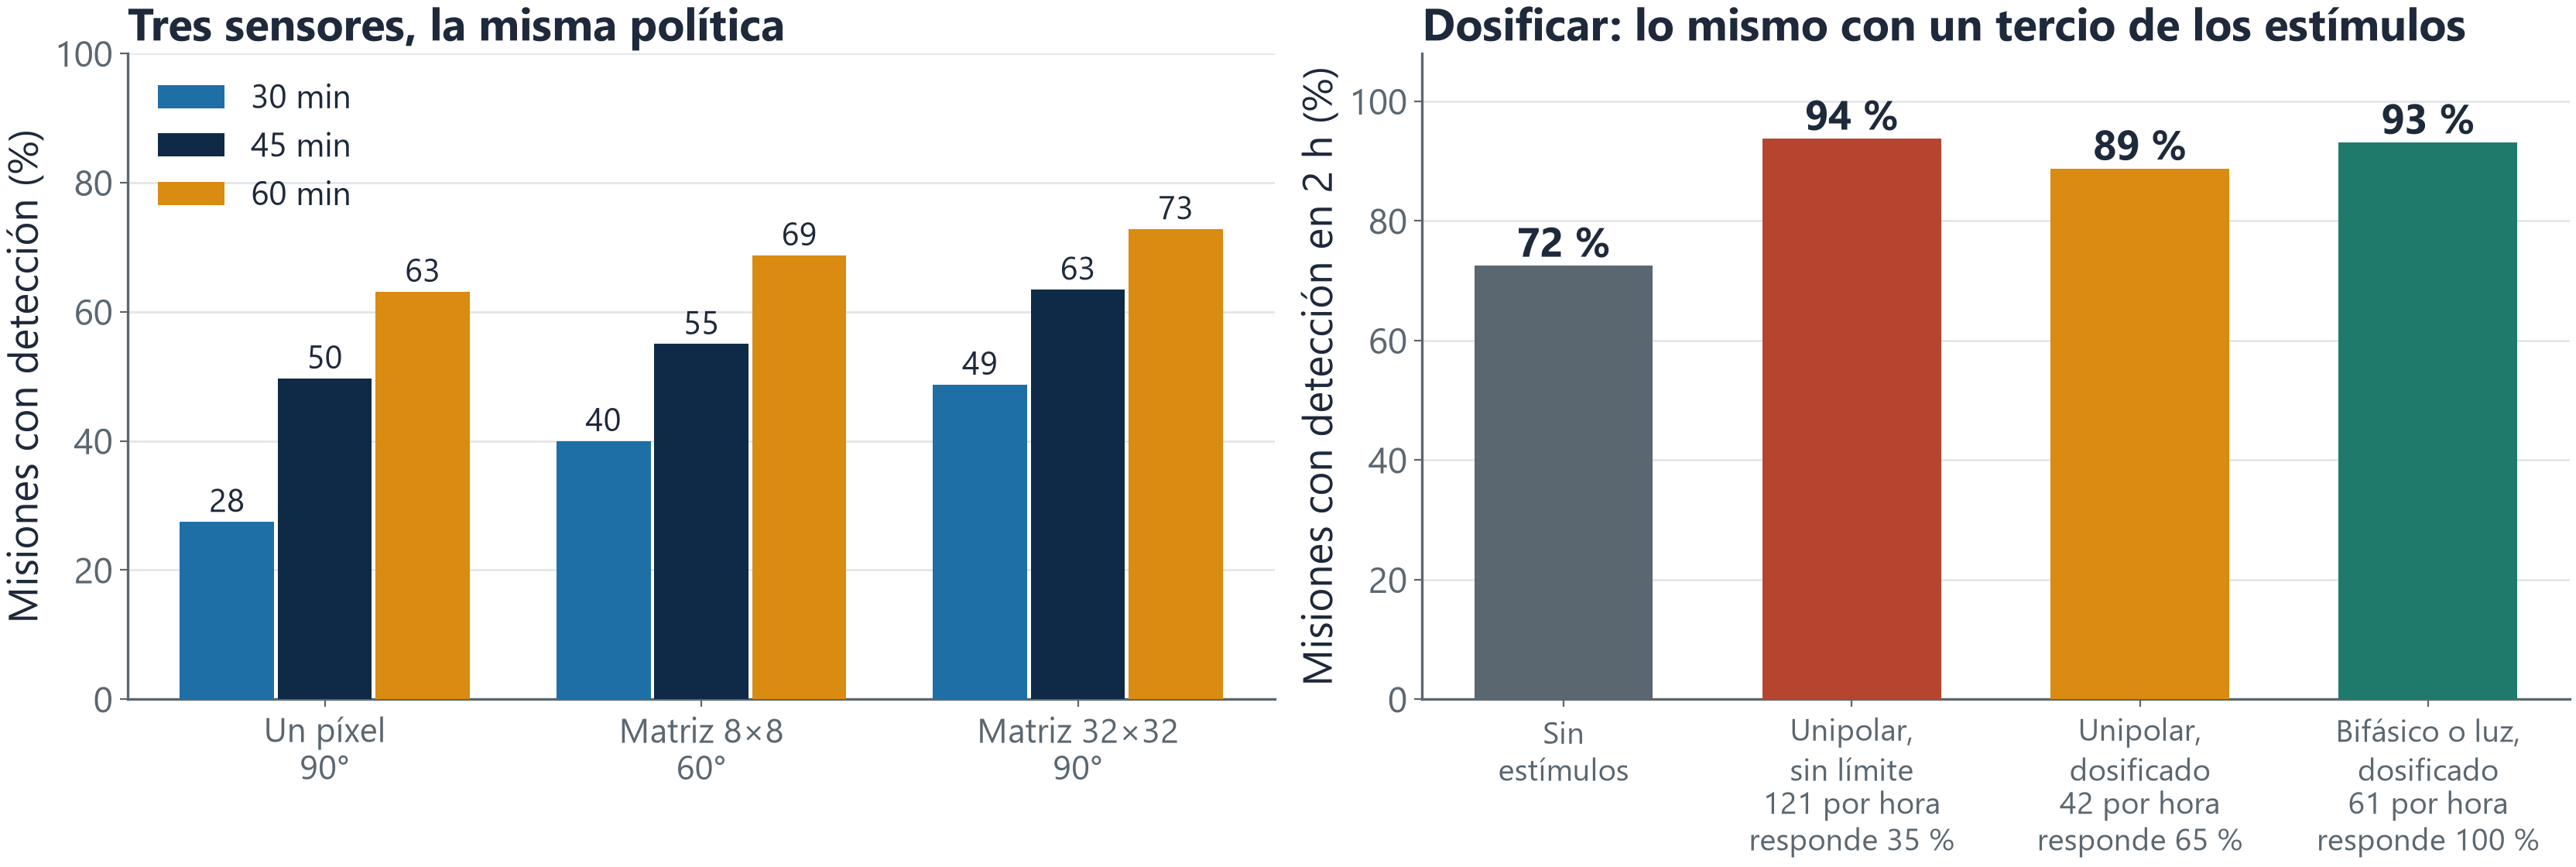
\includegraphics[width=\textwidth]{figs/sensores_habituacion.png}
\caption{Izquierda: política guiada con tres sensores. Derecha: misiones de dos horas con pulsos
unipolares, con y sin dosificación, frente a un estímulo que no habitúa.}
\label{fig:sensorhab}
\end{figure}

\textbf{El sensor cambia el resultado menos que la política.} Con la misma política guiada, la
matriz de $8\times8$ detecta en una hora en \senOchoSesenta~\% de las misiones y la de
$32\times32$ en \senTreintaDosSesenta~\%. La diferencia es mayor al principio: a los 30~min,
\senOchoTreinta{} frente a \senTreintaDosTreinta~\%. La matriz de $8\times8$, que es la que se
consigue en México, pierde pocos puntos y cuesta la mitad. El sensor de un solo punto llega a
\senPixelSesenta~\%, pero ese número lo favorece: la simulación no tiene falsas alarmas, y un
umbral de medio grado sobre el fondo las tendría.

\textbf{Dosificar no mejora la detección: la iguala con un tercio de los estímulos.} En misiones de
dos horas con pulsos unipolares, que son los que habitúan, estimular sin límite aplica
\habEstSinLimite{} estímulos por insecto y por hora y deja la respuesta en
\habRespSinLimite~\%. Con el presupuesto se aplican \habEstDosificado{} y la respuesta queda en
\habRespDosificado~\%. La detección es prácticamente la misma: \habDetSinLimite{} y
\habDetDosificado~\%, dentro del margen de muestreo. El argumento para dosificar es, entonces,
el animal y no el rendimiento: se obtiene lo mismo con la tercera parte de la carga sobre el
insecto. Con un estímulo que no habitúa, como la onda bifásica o la luz, la detección en dos
horas llega a \habDetBifasico~\%, frente a \habDetPasiva~\% sin estímulos.

\subsection{Sensibilidad a los supuestos}

Doce parámetros se movieron entre un valor bajo y uno alto, uno a la vez, en cuatro de los
colapsos (160 misiones por caso; el margen sube a unos $\pm8$ puntos). En esos cuatro colapsos
la referencia es de \sensBaseGuiada~\% de detección a 45~min para la política guiada y de
\sensBasePasiva~\% para la pasiva.

\begin{figure}[H]
\centering
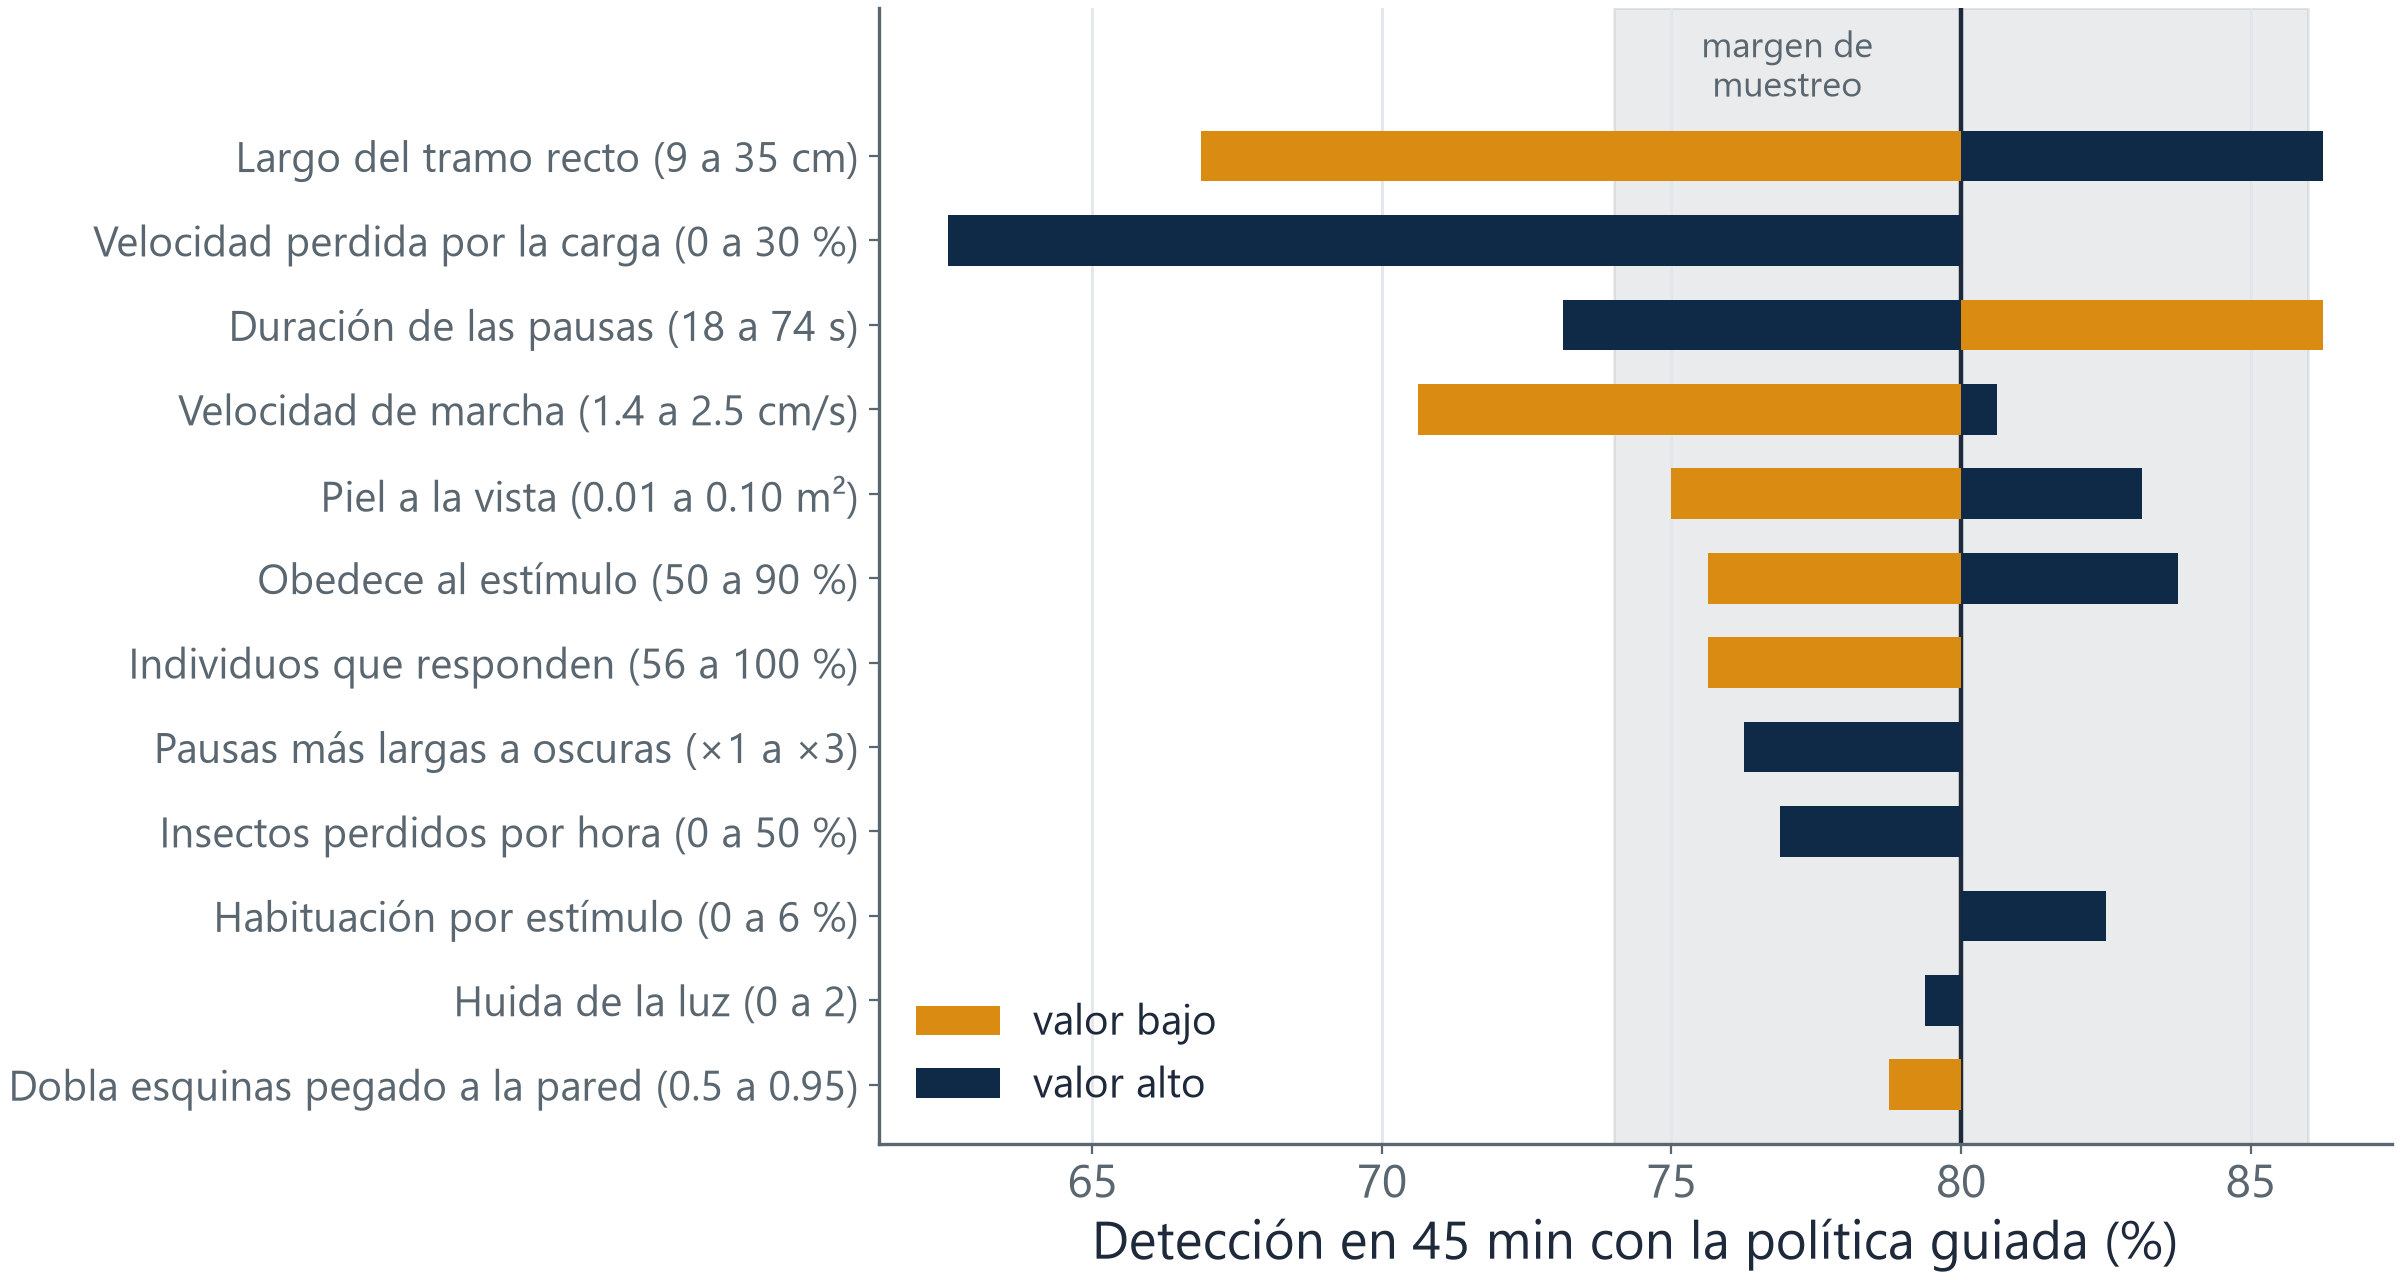
\includegraphics[width=0.86\textwidth]{figs/sensibilidad.png}
\caption{Cambio en la detección a 45~min de la política guiada al mover cada supuesto.}
\label{fig:sensibilidad}
\end{figure}

\begin{table}[H]
\centering\footnotesize
\caption{Detección a 45~min (\%) con el valor bajo y con el valor alto de cada supuesto.}
\label{tab:sensibilidad}
\rowcolors{2}{SoftGray}{white}
\begin{tabularx}{\textwidth}{@{}>{\raggedright\arraybackslash}X >{\raggedright\arraybackslash}p{3.3cm} r r r r@{}}
\toprule
\rowcolor{TableHead} & & \multicolumn{2}{c}{\textbf{Guiada}} & \multicolumn{2}{c}{\textbf{Pasiva}} \\
\rowcolor{TableHead} \textbf{Supuesto} & \textbf{Intervalo} & bajo & alto & bajo & alto \\
\midrule
\tablaSensibilidad
\bottomrule
\end{tabularx}
\end{table}

Cuatro supuestos mueven el resultado más que el margen de muestreo:
\begin{itemize}
  \item \textbf{El largo del tramo recto:} de \sensTramoBajoGuiada{} a \sensTramoAltoGuiada~\%. El insecto
        que camina tramos largos explora mejor. El dato se midió en arena abierta; entre escombro
        podría ser menor.
  \item \textbf{La velocidad que quita la carga:} de \sensCargaBajoGuiada{} a \sensCargaAltoGuiada~\% si la
        mochila le resta 30~\% de velocidad. Es el argumento numérico para la mochila ligera.
  \item \textbf{La duración de las pausas:} de \sensPausaBajoGuiada~\% con pausas cortas a
        \sensPausaAltoGuiada~\% con pausas largas.
  \item \textbf{La velocidad de marcha:} de \sensVelocidadBajoGuiada{} a \sensVelocidadAltoGuiada~\%.
\end{itemize}
Los demás (cuánto obedece, cuántos individuos responden, la habituación, la huida de la luz, la
pérdida de insectos) cambian el resultado menos que el margen de muestreo. De ahí salen dos
lecturas. La política tolera la incertidumbre sobre el estímulo, que es justo lo peor conocido. Y
lo que más importa es cuánto y qué tan rápido camina el insecto, que es lo que la carga y la
temperatura deterioran. Para la política pasiva pesa sobre todo cuánta piel queda a la vista: de
\sensAreaBajoPasiva{} a \sensAreaAltoPasiva~\%.

\subsection{Recuperar a los insectos}
\label{sec:regreso}

Una mochila que no vuelve es un animal abandonado y una pila de litio bajo el escombro. Por eso se
simuló también la segunda mitad de la misión. Tras 45~min de búsqueda guiada se da la orden de
regreso; en el boquete hay un refugio oscuro que retiene a los insectos que pasan a 30~cm de él.
Se siguió a \regInsectos{} insectos por caso durante dos horas más.

\begin{figure}[H]
\centering
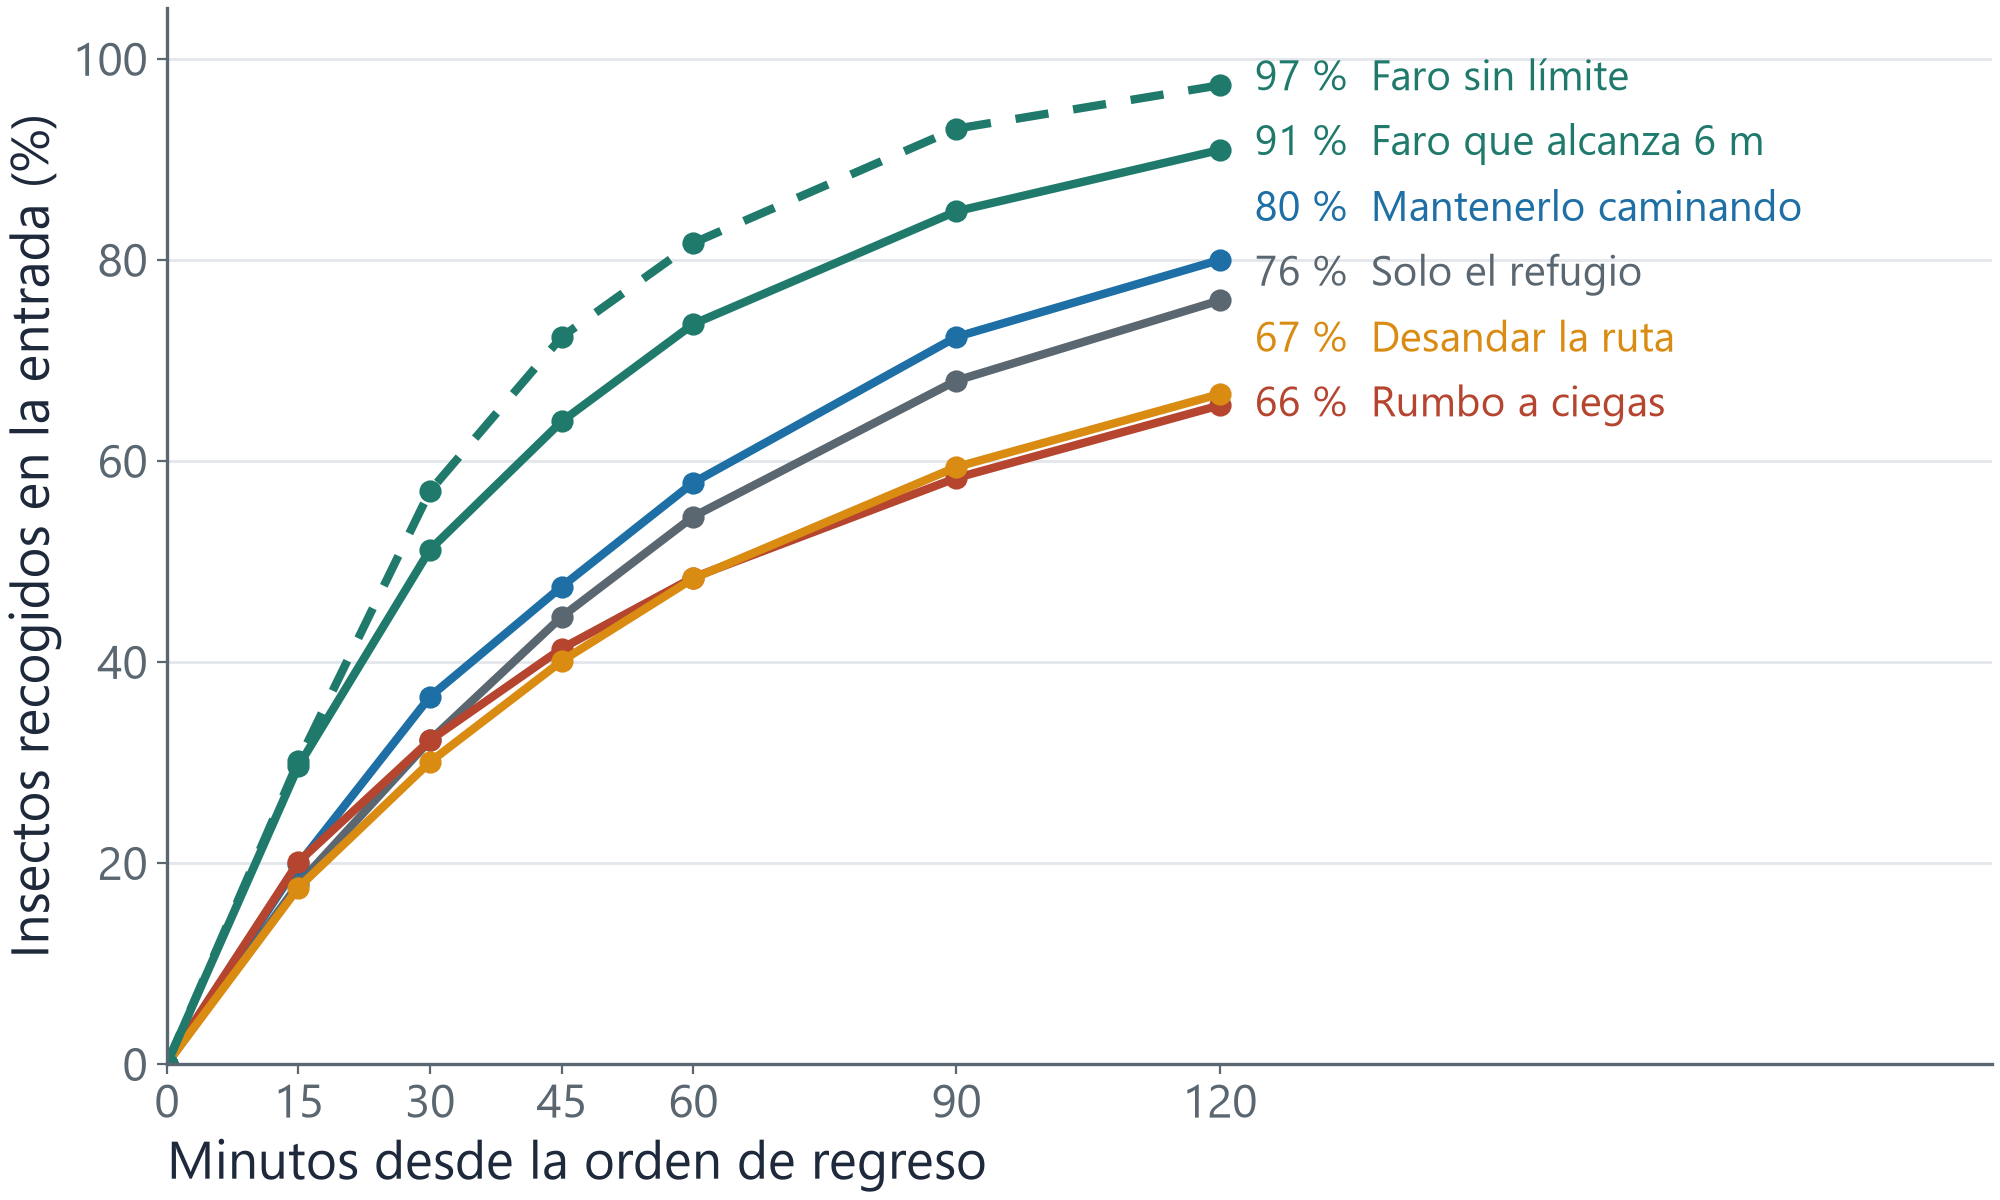
\includegraphics[width=0.74\textwidth]{figs/regreso.png}
\caption{Insectos recogidos en el refugio de la entrada, según la forma de hacerlos volver. La línea
punteada es el faro sin límite de alcance, que no es realista y marca el techo del método.}
\label{fig:regreso}
\end{figure}

\begin{table}[H]
\centering\footnotesize
\caption{Insectos recogidos (\%) después de la orden de regreso y estímulos gastados en volver.}
\label{tab:regreso}
\rowcolors{2}{SoftGray}{white}
\begin{tabularx}{0.9\textwidth}{@{}>{\raggedright\arraybackslash}X r r r r@{}}
\toprule
\rowcolor{TableHead} \textbf{Forma de regresar} & \textbf{30 min} & \textbf{60 min} & \textbf{120 min} & \textbf{Estímulos por insecto} \\
\midrule
\tablaRegreso
\bottomrule
\end{tabularx}
\end{table}

\begin{itemize}
  \item \textbf{Esperar no basta.} Con solo el refugio vuelve \regTrampaSesenta~\% en una hora y
        \regTrampaDos~\% en dos. Darle un pulso cada vez que se detiene sube poco: \regAndarDos~\%.
  \item \textbf{Guiarlo a ciegas es peor que no guiarlo.} La mochila no sabe dónde está: lo estima
        contando pasos y giros, y esa cuenta se desvía con cada metro. Ordenarle el rumbo recto a la
        entrada, o desandar la ruta guardada, recupera \regRumboDos{} y \regRutaDos~\% en dos horas.
        Es menos que el refugio solo, y cuesta \regEstRumbo{} y \regEstRuta{} estímulos por insecto.
  \item \textbf{Lo que cambia el resultado es una señal en la entrada.} Se probó un faro: una lámpara
        infrarroja en el boquete, cuya luz se cuela por los huecos, y un fotodiodo a cada lado de la
        mochila para saber de qué lado llega más. El insecto no ve esa luz; la mochila lo gira hacia
        ella con los mismos estímulos de la búsqueda. Si el faro se percibe hasta 6~m de camino,
        vuelve \regFaroSesenta~\% en una hora y \regFaroDos~\% en dos, con \regEstFaro{} estímulos
        por insecto. Con el doble de error en la medida, \regFaroRuidoDos~\%.
  \item \textbf{Ningún método los recupera a todos.} Con el faro de 6~m queda fuera
        \regFaroPerdidos~\% a las dos horas: de diez mochilas se pierde, en promedio, una por
        misión. Para esas hace falta otra cosa: que cada mochila siga emitiendo su número por
        radio, de modo que se sepa cuántas faltan y cerca de qué relevo quedaron.
\end{itemize}

El faro es un supuesto y no una medida. Nadie ha publicado cuánto se propaga una luz o un sonido
entre escombro, ni con qué error lo localiza una mochila de este tamaño. Sí existen las dos piezas
por separado: una cerca invisible que devuelve al insecto cuando sale de una zona~\cite{latif2014}
y micrófonos en la mochila para localizar una fuente de sonido~\cite{latif2016}. El modo de regreso
tampoco está en el núcleo: pide dos fotodiodos, un comparador y un estado más en la máquina.

\subsection{Qué dice y qué no dice la simulación}

\textbf{Sobre la hipótesis.} Se sostiene en parte. La política guiada aumenta la detección en una
sesión de 45 a 60~min (de \pPasivaCuarentaCinco{} a \pGuiadaCuarentaCinco~\% y de
\pPasivaSesenta{} a \pGuiadaSesenta~\%), no provoca habituación con un estímulo bifásico o de luz
y cabe en una FPGA de miligramos. Pero la mejora no es uniforme: depende del colapso, y en uno
de los ocho la política empeora el resultado. Y dosificar no mejora la detección; solo reduce la
carga sobre el insecto.

\begin{itemize}
  \item \textbf{Dice} que una política sencilla, que cabe en 181 elementos lógicos, mejora la búsqueda
        respecto de soltar a los insectos y esperar, y que lo hace con pocos estímulos.
  \item \textbf{Dice} que el número de insectos y la forma del colapso importan más que la política.
  \item \textbf{No dice} cuánto tardaría un rescate real. Los colapsos son sintéticos y planos, la marcha se
        midió en arenas iluminadas y la respuesta a la luz ultravioleta se supuso igual a la de los
        electrodos de superficie.
  \item \textbf{No dice} nada sobre falsas alarmas: en la simulación la persona es la única fuente de
        calor. Eso se medirá con el sensor real.
\end{itemize}

\needspace{20\baselineskip}
\section{Costos}

\begin{table}[H]
\centering\footnotesize
\caption{Costo de una mochila de prototipo con piezas de mostrador en México (precios del 9 de noviembre
de 2026~\cite{unit}). Con tarjetas de desarrollo no cumple la meta de masa: sirve para validar, no para montar.}
\label{tab:costos}
\rowcolors{2}{SoftGray}{white}
\begin{tabularx}{\textwidth}{@{}>{\raggedright\arraybackslash}X r r@{}}
\toprule
\rowcolor{TableHead} \textbf{Pieza} & \textbf{Con matriz $8\times8$} & \textbf{Con matriz $32\times24$} \\
\midrule
Matriz térmica (AMG8833 o MLX90640) & 599 & 1\,100 \\
Radio y procesador (XIAO nRF52840) & 248 & 248 \\
IMU (MPU6050) & 87 & 87 \\
Batería LiPo de 40~mAh & 41 & 41 \\
Dos LED ultravioleta (paquete de 100: 281) & 6 & 6 \\
Tarjeta, base y adhesivo (estimado) & 50 & 50 \\
\midrule
\textbf{Total por mochila (MXN)} & \textbf{1\,031} & \textbf{1\,532} \\
Equivalente a 18.8 MXN por dólar & 55 USD & 81 USD \\
\bottomrule
\end{tabularx}
\end{table}

Para la demostración del curso solo falta comprar la matriz térmica (599~MXN) y los LED
ultravioleta (281~MXN): la DE10-Lite y el ESP32 ya se tienen. El insecto cuesta de 2 a 15~dólares
por ejemplar en Estados Unidos; no se encontró un precio verificable en México.

\begin{figure}[H]
\centering
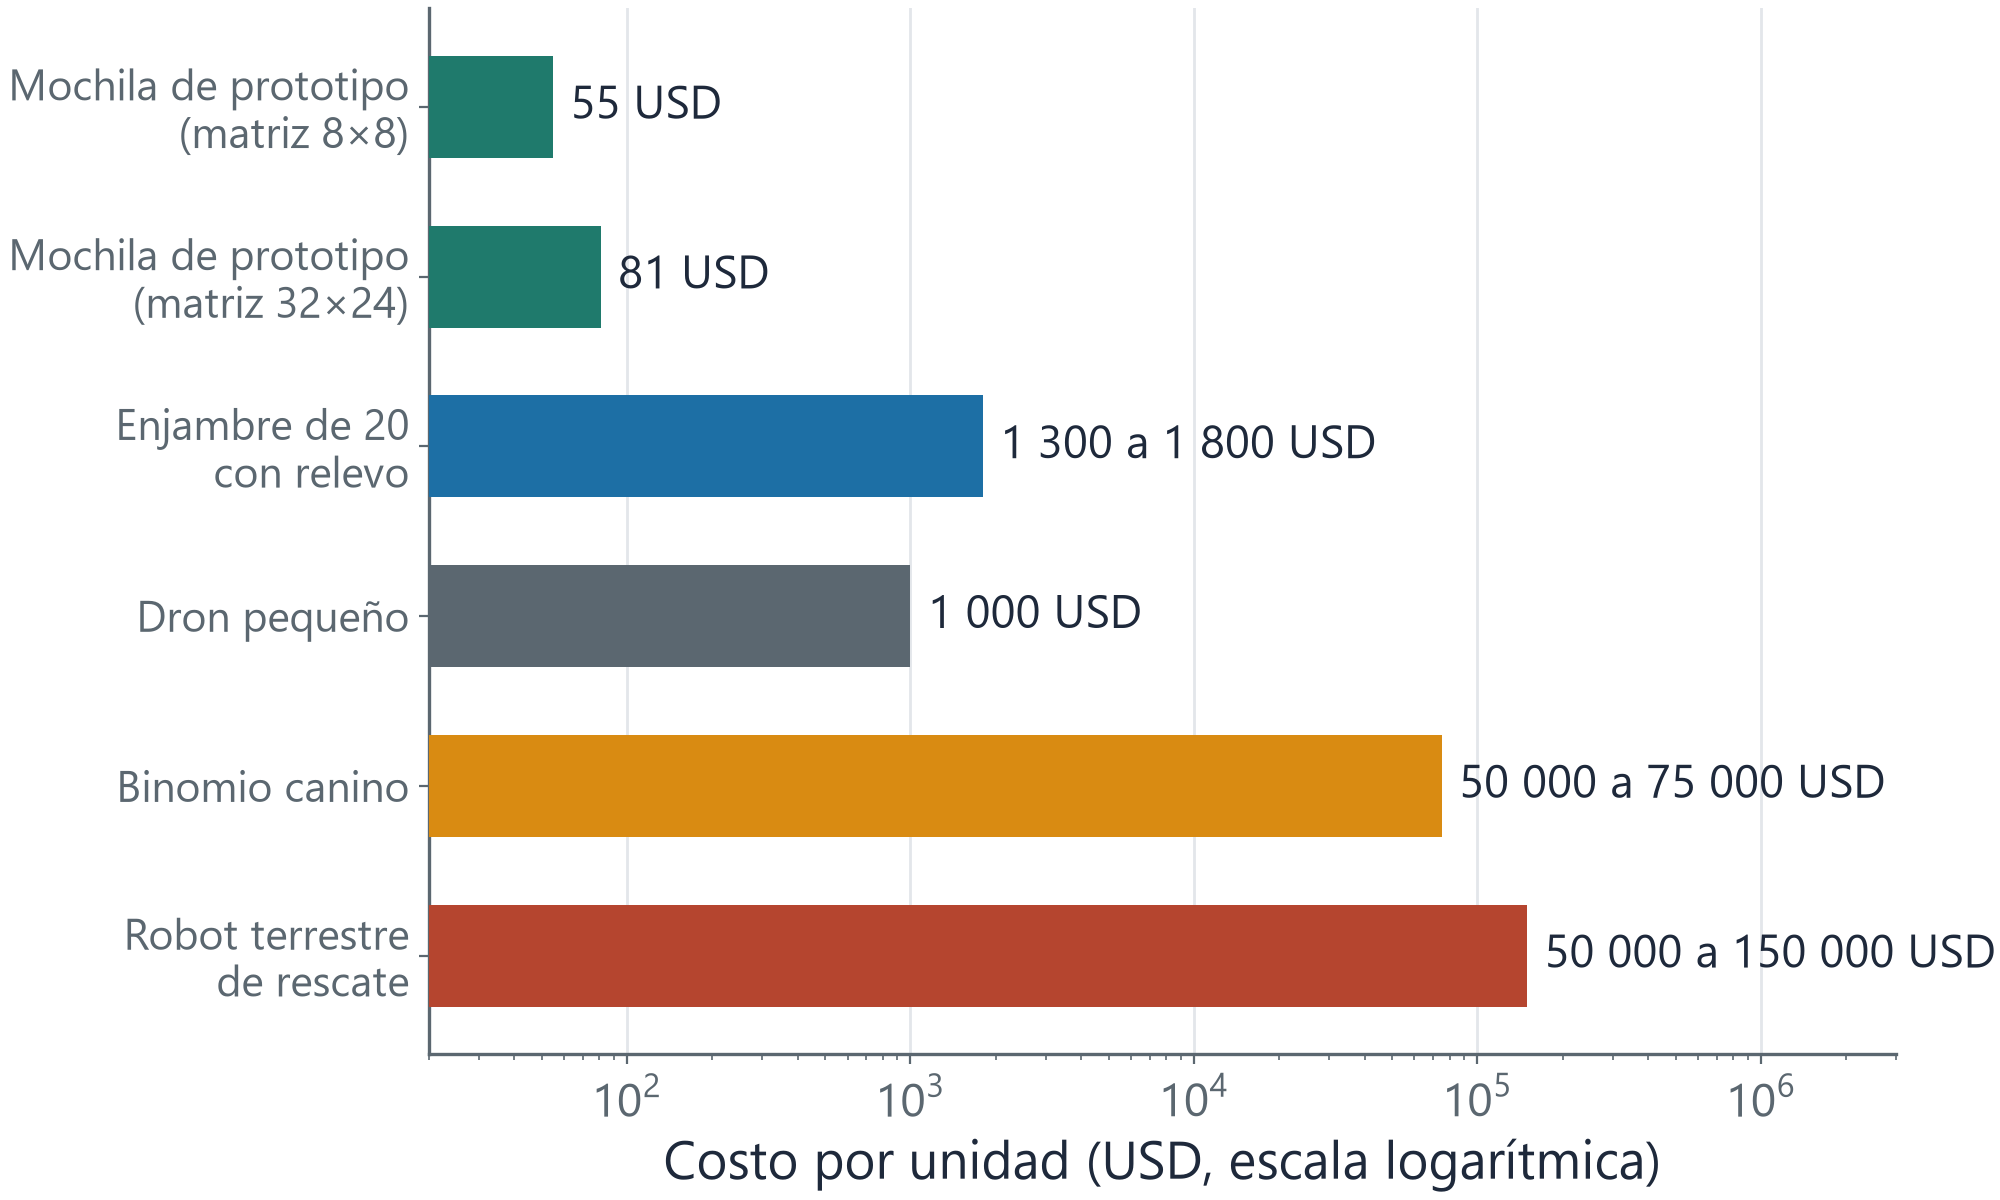
\includegraphics[width=0.72\textwidth]{figs/costos.png}
\caption{Costo por unidad frente a las alternativas. El enjambre de 20 con relevo es una estimación propia
(veinte mochilas más un nodo de radio). Fuentes: \cite{unit,murphy2021,sdf}.}
\label{fig:costos}
\end{figure}

Un enjambre completo cuesta entre 30 y 100 veces menos que un binomio canino o un robot de
rescate, pero la comparación tiene tres salvedades. No son sistemas equivalentes: el perro
encuentra personas y el biobot todavía no lo ha hecho en campo. El costo por unidad oculta la cría, el
personal que monta las mochilas y los permisos. Y la vida útil de cada unidad es corta. El dato
honesto es el costo por hora de búsqueda, que solo se conocerá con pruebas.

\needspace{14\baselineskip}
\section{Practicidad}

La pregunta práctica es si un rescatista podría usarlo. La tabla~\ref{tab:practicidad} cruza lo que
exige el campo con lo que el diseño ofrece.

\begin{table}[H]
\centering\footnotesize
\caption{Requisitos del campo y respuesta del diseño.}
\label{tab:practicidad}
\rowcolors{2}{SoftGray}{white}
\begin{tabularx}{\textwidth}{@{}>{\bfseries\raggedright\arraybackslash}p{3.5cm} >{\raggedright\arraybackslash}X >{\raggedright\arraybackslash}p{4.6cm}@{}}
\toprule
\rowcolor{TableHead} Lo que exige el campo & Cómo responde el diseño & Lo que falta \\
\midrule
Arrancar en menos de 2~min: los rescatistas se van si tarda más~\cite{murphy2004} & La mochila no se configura: se enciende y se suelta el insecto & Medir el tiempo real de preparación \\
No añadir operadores & Nadie pilotea; la estación solo recibe alertas & Probar con rescatistas \\
Sesiones cortas: 45~min en Myanmar~\cite{htx2025} & Autonomía estimada de 4~h & Medir el consumo del prototipo \\
Entrar en rendijas & Insecto de 1.3~cm; mochila de perfil bajo & La matriz térmica mide 5~mm de alto: hay que probar el paso \\
Funcionar con calor y con frío & Solo entre 22 y 30~\textdegree C & Sensor de CO$_2$ para el calor; caja térmica para el transporte \\
Avisar a través del escombro & Radio de menos de 1~GHz con relevo en el boquete & Medir el alcance: nadie lo ha publicado \\
Decir dónde cavar & Entrada conocida, navegación inercial y baliza & Probar el error real \\
Recuperar el equipo y los insectos & Mochilas numeradas; solo machos; conteo de entrada y salida; refugio y faro en el boquete (sección~\ref{sec:regreso}) & En simulación vuelve de \regTrampaDos{} a \regFaroDos~\% en dos horas; con insectos no se ha probado \\
Cumplir la ley & Pruebas en recinto cerrado & Un despliegue real exige autorización: ver la sección~\ref{sec:etica} \\
\bottomrule
\end{tabularx}
\end{table}

\textbf{Cómo se usaría.} El perro marca una zona. El rescatista coloca un relevo de radio en el
boquete, enciende de diez a veinte mochilas y suelta los insectos. Durante 45 a 60~minutos no hace
nada con ellos. Si una mochila alerta, la estación muestra qué insecto fue, por dónde entró y cuánto
caminó. El rescatista confirma con una cámara o con el perro antes de mover una losa. Una búsqueda
sin alertas no descarta que haya alguien: el sistema sirve para encontrar, no para dar por vacía una zona.

\textbf{Lo que el insecto impone.} No se puede contar con él por debajo de unos 20~\textdegree C ni por
encima de 34~\textdegree C; el CO$_2$ concentrado lo anestesia en segundos; bajo el agua sobrevive
minutos; con la mochila se endereza solo entre el 31 y el 82~\% de las veces, según el diseño. Son límites del
animal, no del circuito, y definen dónde el sistema no debe usarse.

\section{Ética, normativa e impacto}
\label{sec:etica}

\subsection{¿Sufre el insecto?}

No hay consenso, y eso obliga a la precaución. Una revisión de más de 300 estudios concluye que las
cucarachas adultas cumplen seis de los ocho criterios usados para evaluar dolor, lo que califica como
evidencia fuerte~\cite{gibbons2022,crump2023}; otros autores sostienen que la nocicepción no implica
dolor y que este es improbable en insectos~\cite{adamo2016}. Ningún artículo de insectos cíborg mide
estrés durante la estimulación ni reporta el destino de los animales. La crítica más dura al campo es
justamente esa: que el animal desaparece de los informes~\cite{dodd2014,mestre2024}.

\subsection{Qué dice la norma en México}

\begin{itemize}
  \item La NOM-062-ZOO-1999 solo cubre roedores, conejos, perros, gatos, primates y cerdos; no menciona
        invertebrados. No hay obligación federal de pasar por un comité de ética~\cite{nom062}. Aun así,
        conviene someter el protocolo de forma voluntaria.
  \item La Ley General de Vida Silvestre sí aplica. La especie es un ejemplar exótico (artículo~3,
        fracción XIV), su manejo solo puede hacerse en confinamiento (artículo~27) y manejarla fuera de
        confinamiento controlado es una infracción (artículo~122, fracción VIII)~\cite{lgvs}.
        \textbf{Un despliegue real en escombros requeriría una autorización que hoy no existe.}
  \item La especie no está en la lista de exóticas invasoras, y las pilas de litio son residuos de manejo
        especial: cada mochila debe recuperarse.
\end{itemize}

\subsection{Protocolo de trato}

\begin{enumerate}
  \item \textbf{Reemplazar.} Todo lo que pueda probarse en simulación o con el circuito en el lazo se prueba
        así. El insecto vivo solo entra para lo que no admite sustituto.
  \item \textbf{Reducir.} El número de insectos se fija antes de empezar y cada individuo aporta varias medidas.
  \item \textbf{Refinar.} Sin cirugía: mochila adherida y estímulo de luz. Si alguna vez se usan electrodos,
        anestesia previa y onda bifásica de 2~V como máximo inicial~\cite{erickson2015}.
  \item Mochila de 3~g como máximo; se verifica que el insecto camina y se endereza con ella; se retira al
        terminar cada sesión.
  \item No más de 12 estímulos acumulados; sesiones de una hora como máximo; descanso de 2~h entre
        sesiones, como en~\cite{gracidas2026}.
  \item Solo machos adultos, doble contención y conteo de entrada y salida. Nunca se liberan.
  \item Punto final: el insecto que no se endereza, deja de comer o muestra una lesión sale del estudio.
        La congelación no es un método de eutanasia válido para esta especie~\cite{tucker2023}.
  \item El reporte declara cuántos insectos se usaron, bajas y destino final~\cite{fischer2024}.
\end{enumerate}

\subsection{Impacto de la solución}

\begin{table}[H]
\centering\footnotesize
\caption{Impacto en los cuatro contextos que pide el resultado de aprendizaje 4 de ABET y el atributo 5 de
CACEI~\cite{abet,cacei}.}
\label{tab:impacto}
\rowcolors{2}{SoftGray}{white}
\begin{tabularx}{\textwidth}{@{}>{\bfseries\raggedright\arraybackslash}p{1.9cm} >{\raggedright\arraybackslash}X >{\raggedright\arraybackslash}X@{}}
\toprule
\rowcolor{TableHead} Contexto & Riesgo & Cómo se atiende \\
\midrule
Global & Doble uso: el campo nació de un programa militar y la misma mochila puede vigilar & Fin humanitario declarado; imagen térmica de baja resolución; sin audio ni grabación \\
Global & Tecnología que solo operan países con laboratorios y permisos & Piezas comerciales, diseño abierto y documentación en español \\
Económico & Costo por unidad bajo que oculta cría, personal y vida útil corta & Reportar el costo por hora de búsqueda cuando se mida \\
Económico & Responsabilidad si el sistema no detecta a alguien & Uso complementario: una búsqueda sin alertas no cierra una zona \\
Ambiental & Escape de una especie exótica & Solo machos, doble contención, cero liberación \\
Ambiental & Tarjetas y pilas de litio abandonadas & Mochilas numeradas y recuperación completa como meta \\
Social & Rechazo de la víctima o del rescatista & Baliza de luz que identifique al dispositivo; ensayos conjuntos con rescatistas \\
Social & Privacidad en viviendas colapsadas & La matriz de 64 píxeles no permite reconocer a una persona \\
\bottomrule
\end{tabularx}
\end{table}

El proyecto responde a la meta 11.5 de los Objetivos de Desarrollo Sostenible (reducir las muertes
por desastres) y a la prioridad~4 del Marco de Sendai (preparación para una respuesta
eficaz)~\cite{ods,sendai}. La meta 13.1 no aplica: un sismo no es un peligro climático. En lo
profesional, el Código de Ética del IEEE obliga a sustentar las afirmaciones en los datos disponibles y a
revelar lo que pueda poner en peligro al público~\cite{ieeecode}; por eso este documento separa lo medido,
lo simulado y lo supuesto.

\section{Metodología y plan de trabajo}

\begin{table}[H]
\centering\footnotesize
\caption{Fases del proyecto.}
\label{tab:fases}
\rowcolors{2}{SoftGray}{white}
\begin{tabularx}{\textwidth}{@{}>{\bfseries\raggedright\arraybackslash}p{3.3cm} >{\raggedright\arraybackslash}X >{\raggedright\arraybackslash}p{4.5cm}@{}}
\toprule
\rowcolor{TableHead} Fase & Qué se hace & Criterio de terminado \\
\midrule
1. Revisión y modelo & Datos publicados, cinco submodelos y simulación de misión & Hecho: este documento \\
2. Núcleo en Verilog & Siete módulos, modelo de referencia, cinco bancos de prueba y prueba en dos DE10-Lite & Hecho: coincidencia total, síntesis sin errores y los cuatro escenarios correctos en las tarjetas \\
3. Sensor y ESP32 & Lectura de la matriz térmica y envío de cuadros por UART & La tarjeta recibe 10 cuadros por segundo sin errores \\
4. Integración & Núcleo en la DE10-Lite con sensor real y con insecto simulado & Detecta una mano a la distancia calculada \\
5. Mediciones & Alcance, falsas alarmas, latencia, recursos y consumo & Tabla de lo medido contra lo calculado \\
6. Insecto vivo (opcional) & Mochila de masa equivalente y estímulo de luz, con el protocolo de la sección~\ref{sec:etica} & Solo con autorización del profesor \\
\bottomrule
\end{tabularx}
\end{table}

\needspace{8\baselineskip}
\textbf{Mediciones previstas y su valor calculado.}
\begin{itemize}
  \item \textbf{Alcance de detección} con una mano y con una cara, a 22~\textdegree C: se esperan 0.9~m para
        confirmar y 1.3~m para empezar a acercarse con la matriz de $8\times8$.
  \item \textbf{Falsas alarmas} con una taza caliente, un foco y la pared asoleada: el criterio de ventana
        debe descartar lo que pase de 38~\textdegree C.
  \item \textbf{Latencia} entre que aparece la mancha y la alerta: ocho cuadros, 0.8~s.
  \item \textbf{Recursos y tiempo}: 722 elementos lógicos y 72~MHz, ya obtenidos; consumo de la tarjeta por medir.
  \item \textbf{Circuito en el lazo}: las mismas misiones de la simulación, con la tarjeta decidiendo los
        estímulos; el resultado debe coincidir con la simulación en software.
\end{itemize}

Si se llega a la fase 6, la plataforma de caminadora esférica con control de temperatura descrita
en~\cite{gracidas2026} permitiría medir el dato que más falta: el ángulo de giro que produce un pulso de
luz ultravioleta de 0.5~s, y cuántos pulsos tolera el insecto antes de habituarse.

\begin{figure}[H]
\centering
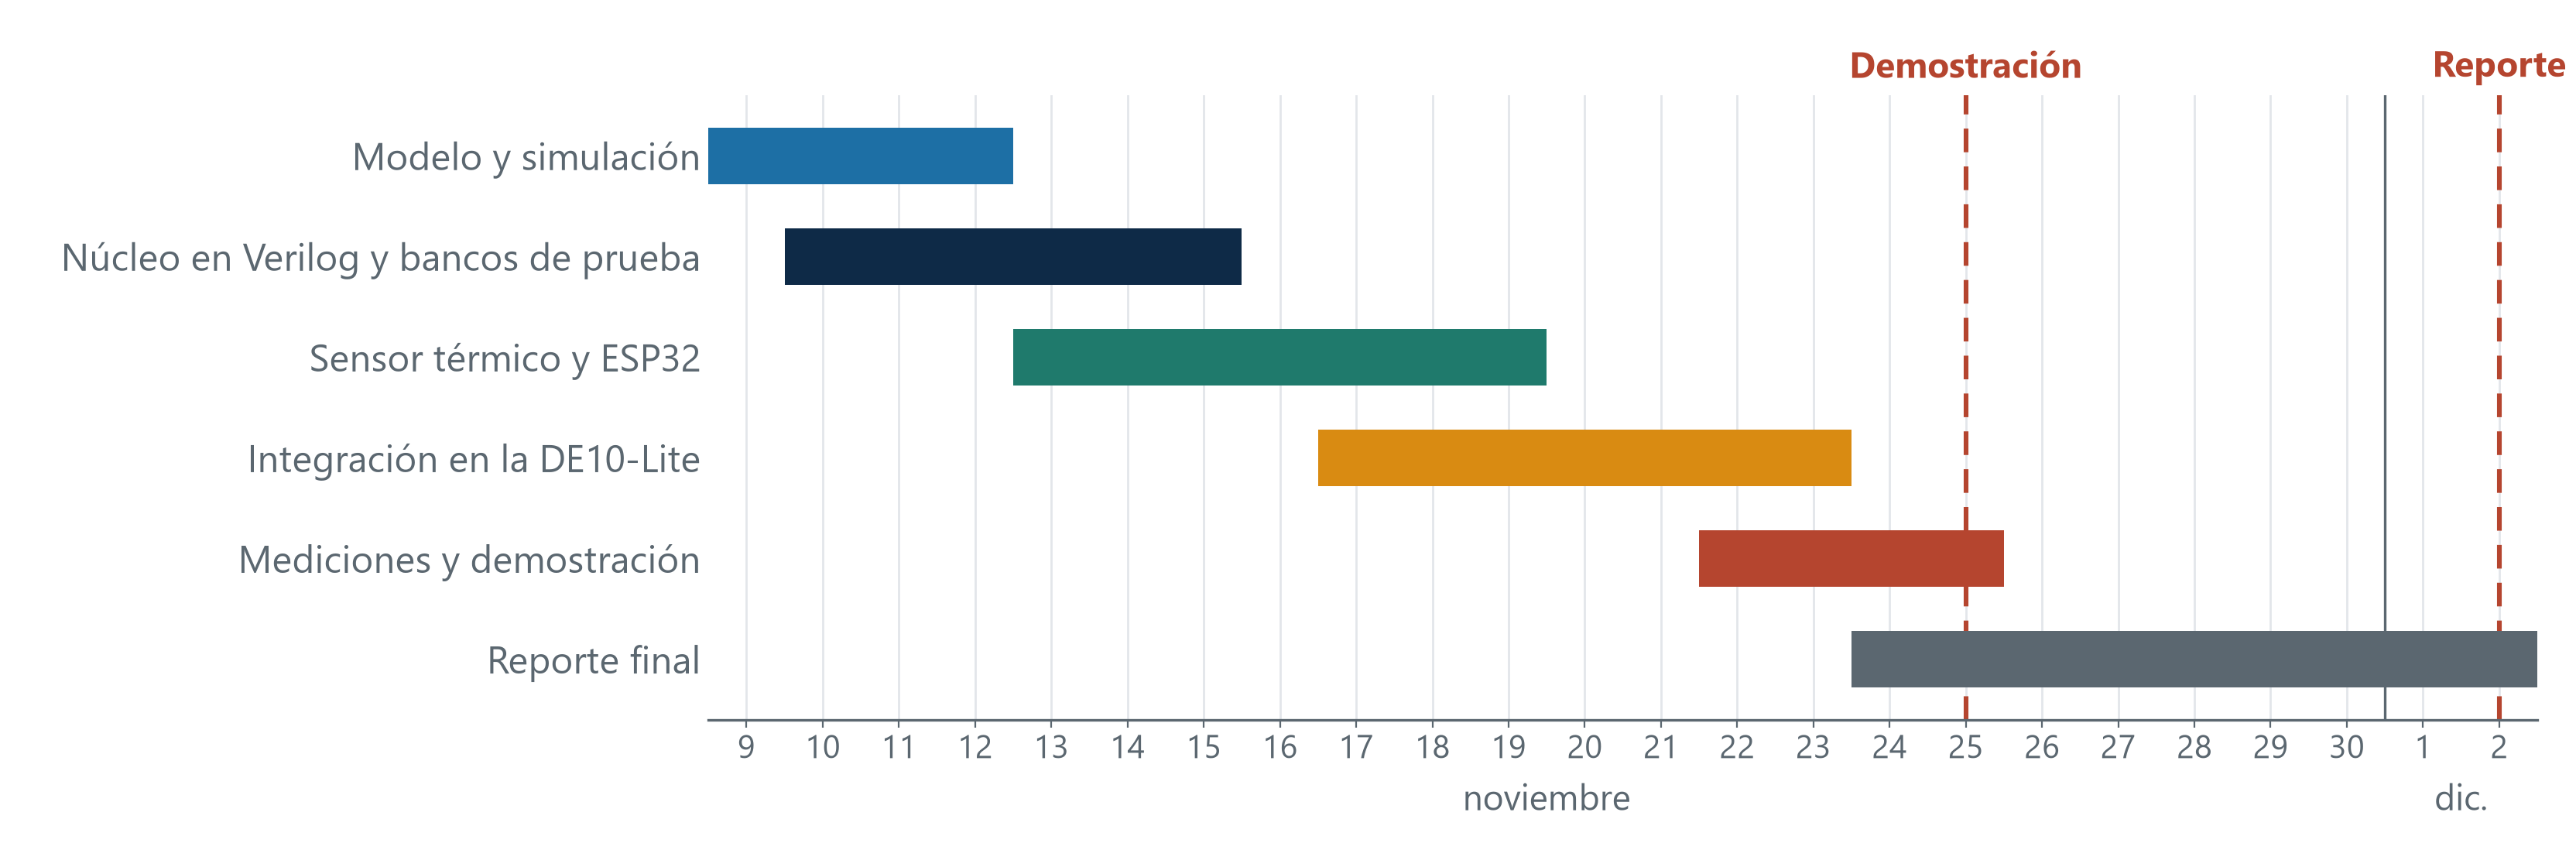
\includegraphics[width=\textwidth]{figs/cronograma.png}
\caption{Cronograma.}
\label{fig:cronograma}
\end{figure}

\needspace{14\baselineskip}
\section{Riesgos y limitaciones}

\begin{table}[H]
\centering\footnotesize
\caption{Riesgos del proyecto y limitaciones del modelo.}
\label{tab:riesgos}
\rowcolors{2}{SoftGray}{white}
\begin{tabularx}{\textwidth}{@{}>{\bfseries\raggedright\arraybackslash}p{4.4cm} >{\raggedright\arraybackslash}X@{}}
\toprule
\rowcolor{TableHead} Riesgo o limitación & Consecuencia y manejo \\
\midrule
La simulación no es un colapso real & Los mapas son sintéticos y en dos dimensiones. Sirve para comparar políticas, no para predecir tiempos de rescate \\
La marcha se midió en arenas iluminadas & No hay datos de marcha a oscuras entre escombro; el análisis de sensibilidad muestra cuánto pesa cada supuesto \\
La respuesta a la luz no está cuantificada & Se usan los valores de electrodos de superficie; la fase 6 lo mediría \\
El ángulo de giro varía de 0 a 110\textdegree{} entre ensayos~\cite{lin2023} & La política no depende de un giro exacto: corrige con el siguiente cuadro \\
La detección falla con ambiente caliente & Límite físico; se documenta y se propone CO$_2$ como señal adicional \\
Recuperar insectos y mochilas está resuelto a medias & En simulación, un refugio y un faro en la entrada recuperan \regFaroDos~\% en dos horas. El faro no se ha medido y siempre queda una parte sin volver; sin esto no hay despliegue responsable \\
La matriz térmica no llega a tiempo & El núcleo se prueba con cuadros que manda una segunda tarjeta por UART, lo que ya funciona en las DE10-Lite \\
La ley exige confinamiento & El proyecto se limita a recinto cerrado \\
\bottomrule
\end{tabularx}
\end{table}

\section{Conclusiones}

\begin{enumerate}
  \item \textbf{El insecto carga menos de lo que se cita.} La meta defendible es una mochila de 2 a 3~g y
        de perfil bajo. La masa del cómputo es despreciable; mandan la batería y el sensor.
  \item \textbf{El estímulo debe ser escaso y sin cirugía.} La luz ultravioleta y los electrodos de superficie
        evitan el implante, y un presupuesto de estímulos acota la habituación con una regla que cabe en
        64 registros.
  \item \textbf{La detección debe contar píxeles, no comparar contra un umbral fijo.} Con una matriz de
        $32\times32$ el acercamiento empieza a 2.5~m y la confirmación ocurre a 1.2~m.
  \item \textbf{El núcleo existe y está verificado.} 477 elementos lógicos y 224 registros, idéntico a su
        modelo de referencia en 11\,424 cuadros, a 72~MHz en la DE10-Lite y con camino a una FPGA de
        2~mg o a un chip propio. En dos tarjetas reales unidas por UART respondió bien a los cuatro
        escenarios: alertó a los 55.1~s con la persona y no alertó en los otros tres.
  \item \textbf{Guiar ayuda, sin milagros.} En la simulación, la política guiada sube la probabilidad de
        detección en una hora de \pPasivaSesenta~\% a \pGuiadaSesenta~\% con diez insectos, y cubre
        \cobGuiada~\% de los huecos frente a \cobPasiva~\%. Diez insectos guiados rinden como entre
        veinte y cuarenta sin guiar. Pesan más el número de insectos y la forma del colapso que la
        política, y girar hacia el calor casi no añade a explorar bien. En uno de los ocho colapsos
        guiar empeora el resultado; un enjambre mixto, mitad guiado y mitad sin estímulos, conserva
        el promedio y evita ese caso.
  \item \textbf{Para que vuelvan hace falta una señal en la entrada.} Esperarlos en un refugio recupera
        \regTrampaDos~\% en dos horas y guiarlos a ciegas, menos. Con un faro que la mochila pueda
        seguir vuelve \regFaroDos~\%. Ningún método los recupera a todos.
  \item \textbf{Los límites son del animal y de la ley.} Temperatura, recuperación y confinamiento definen
        dónde no debe usarse, y decirlo es parte del resultado.
\end{enumerate}

El siguiente paso es la fase 3: conectar la matriz térmica al ESP32 y probar el núcleo con una mano
frente al sensor.

% Referencias en formato IEEE, numeradas por orden de aparición.
\renewcommand{\refname}{Referencias}
{\footnotesize
\begin{thebibliography}{99}
\setlength{\itemsep}{1pt}

\bibitem{kawata} Y. Kawata, «The Great Hanshin-Awaji Earthquake Disaster», \textit{J. Natural Disaster Science}, vol.~17, n.º~2, 1995. Las proporciones por día provienen de un trabajo del mismo autor de 1996, consultado a través de una cita secundaria.
\bibitem{noji} E. K. Noji, «Public health consequences of earthquakes», Supercourse, Universidad de Pittsburgh. [En línea]. Disponible: \url{https://sites.pitt.edu/~super1/lecture/lec13051/013.htm}
\bibitem{macintyre} A. G. Macintyre, J. A. Barbera y E. R. Smith, «Surviving collapsed structure entrapment after earthquakes: a ``time-to-rescue'' analysis», \textit{Prehosp. Disaster Med.}, vol.~21, n.º~1, pp.~4--19, 2006.
\bibitem{japon2014} Gabinete de Japón, \textit{Libro Blanco de Gestión de Desastres 2014}. [En línea]. Disponible: \url{https://www.bousai.go.jp/kaigirep/hakusho/h26/honbun/0b_2s_01_00.html}
\bibitem{ssn2017} Servicio Sismológico Nacional, «Reporte especial: sismo del día 19 de septiembre de 2017, Puebla-Morelos (M 7.1)», UNAM, 2017.
\bibitem{galvis2020} F. Galvis, E. Miranda, P. Heresi, H. Dávalos y J. Ruiz-García, «Overview of collapsed buildings in Mexico City after the 19 September 2017 (Mw7.1) earthquake», \textit{Earthquake Spectra}, 2020, doi: 10.1177/8755293020936694.
\bibitem{murphy2004} R. R. Murphy, «Trial by fire: activities of the rescue robots at the World Trade Center», \textit{IEEE Robot. Autom. Mag.}, vol.~11, n.º~3, pp.~50--61, 2004.
\bibitem{murphy2021} R. R. Murphy, «An expert on search and rescue robots explains the technologies used in disasters like the Florida condo collapse», \textit{The Conversation}, 2021.
\bibitem{whitman2018} J. Whitman \textit{et al.}, «Snake robot urban search after the 2017 Mexico City earthquake», en \textit{Proc. IEEE Int. Symp. Safety, Security, and Rescue Robotics}, 2018.
\bibitem{htx2025} Public Service Division, Gobierno de Singapur, «From lab to rubble», 12 ago. 2026; y «Singapore's cyborg cockroaches helping with search and rescue efforts in Myanmar quake», \textit{The Straits Times}, 5 abr. 2025.
\bibitem{insarag} INSARAG, \textit{Guidelines}, vol.~III, anexo B20, «Assessment, search and rescue levels», OCHA, 2020.
\bibitem{sdf} National Disaster Search Dog Foundation, «Frequently asked questions». [En línea]. Disponible: \url{https://searchdogfoundation.org/about/faqs/}
\bibitem{jpl2015} Jet Propulsion Laboratory, «DHS and NASA technology helps save four in Nepal earthquake disaster», 5 may. 2015.
\bibitem{tranngoc2023} P. T. Tran-Ngoc \textit{et al.}, «Intelligent insect--computer hybrid robot: installing innate obstacle negotiation and onboard human detection onto cyborg insect», \textit{Adv. Intell. Syst.}, vol.~5, n.º~5, 2200319, 2023.
\bibitem{latif2012} T. Latif y A. Bozkurt, «Line following terrestrial insect biobots», en \textit{Proc. IEEE EMBC}, 2012, pp.~972--975.
\bibitem{erickson2015} J. C. Erickson, M. Herrera, M. Bustamante, A. Shingiro y T. Bowen, «Effective stimulus parameters for directed locomotion in Madagascar hissing cockroach biobot», \textit{PLoS ONE}, vol.~10, n.º~8, e0134348, 2015.
\bibitem{sanchez2015} C. J. Sanchez, C.-W. Chiu, Y. Zhou, J. M. González, S. B. Vinson y H. Liang, «Locomotion control of hybrid cockroach robots», \textit{J. R. Soc. Interface}, vol.~12, 20141363, 2015.
\bibitem{dirafzoon2017} A. Dirafzoon, T. Latif, F. Gong, M. Sichitiu, A. Bozkurt y E. Lobaton, «Biobotic motion and behavior analysis in response to directional neurostimulation», en \textit{Proc. IEEE ICASSP}, 2017, pp.~2457--2461.
\bibitem{kakei2022} Y. Kakei \textit{et al.}, «Integration of body-mounted ultrasoft organic solar cell on cyborg insects with intact mobility», \textit{npj Flex. Electron.}, vol.~6, 78, 2022.
\bibitem{lin2023} Q. Lin \textit{et al.}, «Resilient conductive membrane synthesized by in-situ polymerisation for wearable non-invasive electronics on moving appendages of cyborg insect», \textit{npj Flex. Electron.}, vol.~7, 42, 2023.
\bibitem{ma2023} S. Ma, Y. Chen, S. Yang, S. Liu, L. Tang, B. Li y Y. Li, «The autonomous pipeline navigation of a cockroach bio-robot with enhanced walking stimuli», \textit{Cyborg Bionic Syst.}, vol.~4, 0067, 2023.
\bibitem{bai2025} Y. Bai \textit{et al.}, «Swarm navigation of cyborg-insects in unknown obstructed soft terrain», \textit{Nat. Commun.}, vol.~16, 221, 2025.
\bibitem{lin2025} Q. Lin \textit{et al.}, «Cyborg insect factory: automatic assembly for insect-computer hybrid robot via vision-guided robotic arm manipulation of custom bipolar electrodes», \textit{Nat. Commun.}, vol.~16, 6073, 2025.
\bibitem{refat2025} C. M. M. Refat, M. Ariyanto, R. Tanaka, K. Yamamoto y K. Morishima, «Autonomous navigation of bio-intelligent cyborg insect based on insect visual perception», \textit{Adv. Intell. Syst.}, vol.~7, n.º~10, 2400838, 2025.
\bibitem{gracidas2026} E. Gracidas-Reyes, G. Diaz-Arango, H. Vazquez-Leal y F. Marroquin-Gutierrez, «Temperature-dependent tethered locomotion behavior in the Madagascar hissing cockroach using a controlled-environment treadmill platform with exploratory illumination assays», \textit{Biology}, vol.~15, n.º~12, 947, 2026.
\bibitem{li2019} C. Li, T. Wöhrl, H. K. Lam y R. J. Full, «Cockroaches use diverse strategies to self-right on the ground», \textit{J. Exp. Biol.}, vol.~222, jeb186080, 2019.
\bibitem{kai2026} K. Kai, L. D. Long, Q. Lin y H. Sato, «Fully implanted miniature radio controller boosts cyborg insect mobility in challenging terrains», \textit{Cyborg Bionic Syst.}, vol.~7, 0589, 2026.
\bibitem{montagut2024} M. J. Montagut Marques \textit{et al.}, «Cyborg insect repeatable self-righting locomotion assistance using bio-inspired 3D printed artificial limb», \textit{npj Robot.}, vol.~2, 3, 2024.
\bibitem{tranngoc2024} P. T. Tran-Ngoc, H. D. Nguyen, D. L. Le, R. Li, B. S. Chong y H. Sato, «Gait-adaptive navigation and human searching in field with cyborg insect», arXiv:2406.03713, 2024.
\bibitem{herreid1981} C. F. Herreid, R. J. Full y D. A. Prawel, «Energetics of cockroach locomotion», \textit{J. Exp. Biol.}, vol.~94, pp.~189--202, 1981.
\bibitem{mcgorry2014} C. A. McGorry, C. N. Newman y J. D. Triblehorn, «Neural responses from the wind-sensitive interneuron population in four cockroach species», \textit{J. Insect Physiol.}, vol.~66, pp.~59--70, 2014.
\bibitem{yoder1997} J. A. Yoder y N. C. Grojean, «Group influence on water conservation in the giant Madagascar hissing-cockroach», \textit{Physiol. Entomol.}, vol.~22, pp.~79--82, 1997.
\bibitem{tranngoc2025} P. T. Tran-Ngoc, K. Song, T. H. Tran, K. Kai, Q. Lin y H. Sato, «Ergonomic insect headgear and abdominal buckle with surface stimulators manufactured via multimaterial 3D printing», \textit{Cyborg Bionic Syst.}, vol.~6, 0406, 2025.
\bibitem{nordic} Nordic Semiconductor, «nRF52840 SoC product brief», versión 2.3.
\bibitem{lattice} Lattice Semiconductor, «iCE40 UltraPlus family data sheet», FPGA-DS-02008, 2025; e «iCE40 Ultra / UltraLite».
\bibitem{tinytapeout} Tiny Tapeout. [En línea]. Disponible: \url{https://tinytapeout.com} (consultado el 9 nov. 2026).
\bibitem{unit} UNIT Electronics, catálogo en línea. Disponible: \url{https://uelectronics.com} (precios consultados el 9 nov. 2026).
\bibitem{melexis} Melexis, hojas de datos «MLX90614» y «MLX90640 $32\times24$ IR array».
\bibitem{panasonic} Panasonic, «Infrared array sensor Grid-EYE (AMG88)», hoja de datos, 2019.
\bibitem{huo2011} R. Huo \textit{et al.}, «The trapped human experiment», \textit{J. Breath Res.}, vol.~5, n.º~4, 046006, 2011.
\bibitem{itu2040} UIT-R, «Efectos de los materiales y estructuras de construcción en la propagación de las ondas radioeléctricas por encima de unos 100~MHz», Rec. P.2040-1, 2015.
\bibitem{stone1997} W. C. Stone, «Electromagnetic signal attenuation in construction materials», NISTIR 6055, 1997.
\bibitem{frost2001} J. R. Frost y L. D. Stone, «Review of search theory: advances and applications to search and rescue decision support», U.S. Coast Guard, CG-D-15-01, 2001.
\bibitem{skywater} SkyWater Technology y Google, «SKY130 process design kit», biblioteca \texttt{sky130\_fd\_sc\_hd}. [En línea]. Disponible: \url{https://github.com/google/skywater-pdk}
\bibitem{latif2014} T. Latif \textit{et al.}, «Towards fenceless boundaries for solar powered insect biobots», en \textit{Proc. IEEE EMBC}, 2014, pp.~1670--1673.
\bibitem{latif2016} T. Latif, E. Whitmire, T. Novak y A. Bozkurt, «Sound localization sensors for search and rescue biobots», \textit{IEEE Sensors J.}, vol.~16, n.º~10, pp.~3444--3453, 2016.
\bibitem{gibbons2022} M. Gibbons, A. Crump, M. Barrett, S. Sarlak, J. Birch y L. Chittka, «Can insects feel pain? A review of the neural and behavioural evidence», \textit{Adv. Insect Physiol.}, pp.~155--229, 2022.
\bibitem{crump2023} A. Crump, M. Gibbons, M. Barrett, J. Birch y L. Chittka, «Is it time for insect researchers to consider their subjects' welfare?», \textit{PLoS Biol.}, vol.~21, n.º~6, e3002138, 2023.
\bibitem{adamo2016} S. A. Adamo, «Do insects feel pain? A question at the intersection of animal behaviour, philosophy and robotics», \textit{Anim. Behav.}, vol.~118, pp.~75--79, 2016.
\bibitem{dodd2014} A. Dodd, «The trouble with insect cyborgs», \textit{Society \& Animals}, vol.~22, n.º~2, pp.~153--173, 2014.
\bibitem{mestre2024} R. Mestre, A. M. Astobiza, V. A. Webster-Wood, M. Ryan y M. T. A. Saif, «Ethics and responsibility in biohybrid robotics research», \textit{Proc. Natl. Acad. Sci.}, vol.~121, n.º~31, 2024.
\bibitem{nom062} «NOM-062-ZOO-1999, Especificaciones técnicas para la producción, cuidado y uso de los animales de laboratorio», \textit{Diario Oficial de la Federación}, 22 ago. 2001.
\bibitem{lgvs} «Ley General de Vida Silvestre», última reforma publicada en el \textit{Diario Oficial de la Federación} el 16 jul. 2025.
\bibitem{tucker2023} S. M. Tucker, J. A. Balko, D. C. Smith, L. J. Minter y E. M. Houck, «Investigation of euthanasia techniques in four species of cockroaches», \textit{PeerJ}, vol.~11, e16199, 2023.
\bibitem{fischer2024} B. Fischer \textit{et al.}, «Guidelines for protecting and promoting insect welfare in research», Insect Welfare Research Society, 2024.
\bibitem{abet} ABET, \textit{Criteria for Accrediting Engineering Programs, 2026--2027}, Engineering Accreditation Commission, 2025.
\bibitem{cacei} CACEI, \textit{Marco de Referencia 2018 para la acreditación de programas de ingeniería}, versión 3, 2020.
\bibitem{ods} Naciones Unidas, «Objetivos de Desarrollo Sostenible», meta 11.5. [En línea]. Disponible: \url{https://sdgs.un.org/goals/goal11}
\bibitem{sendai} Naciones Unidas, \textit{Marco de Sendai para la Reducción del Riesgo de Desastres 2015--2030}, 2015.
\bibitem{ieeecode} IEEE, «IEEE Code of Ethics», IEEE Policies, sección 7.8, 2020.

\end{thebibliography}}


\end{document}
